%!TEX program = xelatex
%!TEX root = informe
\documentclass[12pt,titlepage,openright]{report}
\usepackage{geometry}
\geometry{a4paper}
\usepackage{graphicx}
\usepackage{amsmath}
\usepackage{amssymb}
\usepackage{url}
\usepackage[colorlinks=false]{hyperref}
\usepackage{bookmark}
\usepackage{siunitx}
\usepackage{booktabs}
\usepackage{appendix}
\usepackage[spanish]{minitoc}
\usepackage{tikz}
\usetikzlibrary{shapes.geometric,arrows,chains}
\usepackage[version=3]{mhchem}
\usepackage{wrapfig}
\usepackage{ccaption}
\usepackage{picinpar}
\usepackage{listings}
\usepackage{multirow}
\frenchspacing
\linespread{1.3}
\usepackage{ifxetex}
\ifxetex
  \usepackage{fontspec,xltxtra,xunicode,unicode-math}
  \usepackage{polyglossia}
  \setmainlanguage{spanish}
  \setmainfont[Mapping={tex-text},Numbers={Lining},Ligatures={Common},BoldFont={Minion Pro Semibold},BoldItalicFont={Minion Pro Semibold Italic}]{Minion Pro}
  \setsansfont[Mapping={tex-text},Colour={AA0000}]{Myriad Pro}
  \setmonofont[Mapping={tex-text},Scale={0.9}]{Inconsolata-g}
  \setmathfont[Mapping={tex-text},Numbers={Lining},Ligatures={Common},BoldFont={Minion Pro Semibold},BoldItalicFont={Minion Pro Semibold Italic}]{Minion Pro}
\else
	\usepackage[T1]{fontenc}
	\usepackage[utf8]{inputenc}
	\usepackage{lmodern}
	\usepackage[activeacute,spanish]{babel}
\fi
\setlength{\headheight}{15pt}
\usepackage{fancyhdr}
\lhead{}
\rhead{\itshape\nouppercase\leftmark}
\chead{}\cfoot{}
\lfoot{\itshape\nouppercase Análisis de Ciclo de Vida de un adoquín.\ \itshape\nouppercase\thepart\ \parttitle .}
\rfoot{\rmfamily\thepage}
\pagestyle{fancy}

\tikzstyle{startstop} = [rectangle, rounded corners, minimum width=3cm, minimum height=1cm,text centered, draw=black, fill=red!30]
\tikzstyle{io} = [trapezium, trapezium left angle=70, trapezium right angle=110, minimum width=3cm, minimum height=1cm, text centered, draw=black, fill=blue!30]
\tikzstyle{process} = [rectangle, minimum width=3cm, minimum height=1cm, text centered, text width=3cm, draw=black, fill=orange!30]
\tikzstyle{decision} = [diamond, minimum width=3cm, minimum height=1cm, text centered, draw=black, fill=green!30]
\tikzstyle{arrow} = [thick,->,>=stealth]

% Bibliography as a section and numbered
\def\thebibliography#1{\section{Bibliografía}%
    \markboth{Bibliografía}{Bibliografía}
  \list{[\arabic{enumi}]}{\settowidth\labelwidth{[#1]}\leftmargin
\labelwidth
    \advance\leftmargin\labelsep
    \usecounter{enumi}}
    \def\newblock{\hskip .11em plus .33em minus .07em}
    \sloppy\clubpenalty4000\widowpenalty4000
    \sfcode`\.=1000\relax}

\begin{document}
\renewcommand\listtablename{Índice de tablas}
\renewcommand\tablename{Tabla}
\renewcommand\appendixname{Anexo}
\nocite{*}
\renewcommand{\footrulewidth}{0.4pt}
\newcommand*\parttitle{}
\let\origpart\part
\renewcommand*{\part}[2][]{%
   \ifx\\#1\\% optional argument not present?
      \origpart{#2}%
      \renewcommand*\parttitle{#2}%
   \else
      \origpart[#1]{#2}%
      \renewcommand*\parttitle{#1}%
   \fi
}

\begin{titlepage}
\begin{center}
{\centering 
\includegraphics{portada.png}}
\vfill
{\LARGE UNIVERSIDAD DE MÁLAGA\\
ESCUELA TÉCNICA SUPERIOR DE\\[10pt]
INGENIEROS INDUSTRIALES}\\[25pt]
{\large DTO. DE EXPRESIÓN GRÁFICA, DISEÑO Y PROYECTOS\\
ÁREA DE EXPRESIÓN GRÁFICA EN LA INGENIERÍA}
\vfill
{\Large PROYECTO FINAL DE CARRERA\\[10pt]
ANÁLISIS DE CICLO DE VIDA DE UN ADOQUÍN}
\end{center}
\vfill
\begin{flushright}
Alumno: Francisco Pinto Oliver\\
Directora: María Luz García Ceballos\\
Ponente: José Ramón de Andrés Díaz\\
Titulación: Ingeniero Industrial
\end{flushright}
\end{titlepage}

\doparttoc
\pagenumbering{roman} \tableofcontents \newpage \listoffigures
\newpage \listoftables \newpage \pagenumbering{arabic}

\chapter*{Agradecimientos}
\begin{flushright}
A la directora de este proyecto,\\por su inestimable ayuda.\\[10pt]
A mi familia y amigos,\\por esos buenos momentos.\\[10pt]
A María y Daniel,\\sin vosotros no sería lo mismo.
\end{flushright}
\vfill

\cleardoublepage

\part{Memoria}
\parttoc
%!TEX root = informe.tex
\chapter{Objeto}
El objetivo principal de este proyecto es el Análisis de Ciclo de Vida del adoquín común prefabricado del cemento utilizado en obras civiles y urbanismo. Se desea analizar el ciclo de vida del adoquín desde la obtención de la materia prima hasta su fin de vida.

Con este Análisis de Ciclo de Vida se pretende evaluar el comportamiento ambiental de las distintas etapas de su ciclo de vida, las cargas ambientales asociadas a estas etapas e identificar las posibles mejoras.

Para poder conseguir estos objetivos, se pueden establecer los siguientes objetivos básicos:
\begin{itemize}
\item Estudio y análisis de los procesos productivos, de instalación, mantenimiento y reciclado de los adoquines.
\item Análisis de las diferentes metodologías de Análisis de Ciclo de Vida.
\item Elección de una unidad de referencia del producto a partir de la cual se puedan normalizar los datos de entrada y salida y que permita su comparación con otros productos o con etapas de su ciclo de vida del mismo.
\item Desarrollo de un inventario de materiales y procesos de cada etapa del ciclo de vida.
\item Conocer y evaluar los impactos ambientales asociados a cada una de las etapas del producto y a su ciclo completo.
\end{itemize}

A su vez, la redacción del presente proyecto bajo la dirección del Departamento de Expresión Gráfica, Diseño y Proyectos de la Universidad de Málaga tiene como finalidad última la obtención del título de Ingeniero Industrial.

%!TEX root = informe.tex
\chapter{Alcance}

En este proyecto se analiza la posibilidad de aprovechar la radiación solar, para la producción de energía eléctrica, en ubicaciones situadas en España y Rumanía, mediante centrales fotovoltaicas conectadas con la red eléctrica.

En el capítulo tres se presenta el consumo de energía eléctrica en el mundo. Para Es- paña se presenta también la evolución de la producción de energía eléctrica en función de su origen y se hace una previsión de la misma para el año 2008. Se hace una presentación de las energías renovables y de su nivel de implantación a nivel mundial, remarcando la energía solar fotovoltaica en España y Rumanía. A continuación, se presentan los principa- les componentes de una central fotovoltaica.

El capítulo cuatro muestra las fuentes de información utilizadas para la realización del proyecto.

En requisitos de diseño (capítulo 6) se presentan las dos ubicaciones inicialmente elegidas para el análisis: Tarragona y Bucarest.

El capitulo siete, análisis de soluciones, presenta los datos de radiación solar y tem- peratura para las dos ubicaciones elegidas inicialmente y también se buscan las ubicaciones con mayor radiación solar en España y Rumanía, presentando también en este caso la ra- diación solar y temperatura. Por último, se hace un análisis económico de las centrales fo- tovoltaicas emplazadas en cada ubicación para determinar el grado de rentabilidad de la inversión en cada caso. Finalmente, el capítulo ocho presenta las mejores soluciones, tanto técnicas como económicas.

%!TEX root = informe.tex
\chapter{Antecedentes}\label{cap:antecedentes}

\section{Introducción}\label{sec:introantecedentes}
La mayoría de las ciudades europeas utilizan materiales prefabricados basados en el cemento para urbanizar el terreno transformándolo en espacio público que utilizarán los ciudadanos. Estas instalaciones deben ser resistentes, económicas, funcionales y sobre todo sostenibles. La sostenibilidad es un requisito que ha ido ganando importancia en los últimos años debido no sólo al aspecto económico —costes y mantenimiento principalmente— sino también al medioambiental.

El impacto medioambietal que producen las actividades humanas en la naturaleza debería convertirse en un elemento más de estudio en cualquier proyecto de ingeniería actual. Para el caso de este proyecto, el sector de las obras civiles y urbanismo supone un consumo muy elevado de materias primas y energía —y representa un porcentaje importante del Producto Interior Bruto de España—, lo que implica altas emisiones al medio ambiente \cite{minetur}.

La incorporación de criterios ambientales en la fase de diseño de un producto y/o servicio se denomina \textit{ecodiseño}. El ecodiseño surge como respuesta a la necesidad de introducir estos criterios durante todo el ciclo de vida de un producto con el objetivo de prevenir o reducir su impacto ambiental —principalmente minimizar los residuos, emisiones y costes energéticos \cite{iso14006}. El ecodiseño es el eslabón clave hacia la sostenibilidad y el consumo responsable ya que incorpora nuevos conceptos como la visión de producto-sistema y el ciclo de vida e integra aspectos económicos y sociales como la ecoeficiencia y el ecodiseño sostenible \cite{ihobeeco}.

La metodología del Análisis de Ciclo de Vida (ACV) permite cuantificar todos los procesos relacionados con un producto y/o servicio desde el punto de vista de las \textit{entradas} —materias primas y energía— y \textit{salidas} —emisiones a la tierra, mar o aire y residuos— en el sistema, identificar los puntos clave y establecer una \textbf{estrategia de mejora} \cite{iso14040}.

\begin{figure}[!htb]
\centering
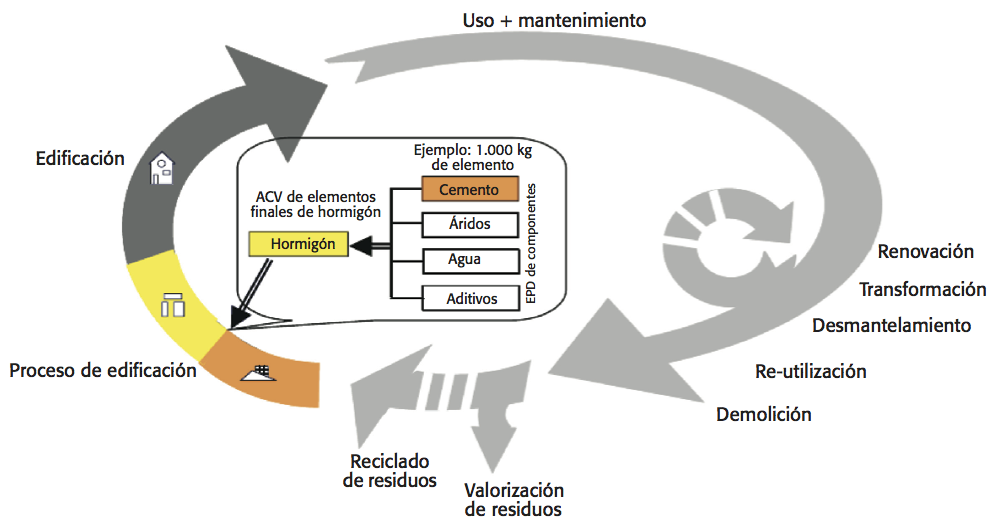
\includegraphics[width=12cm]{img/ciclodevida.png}
\caption[Ciclo de vida de los prefabricados de cemento.]{Ciclo de vida de los prefabricados de cemento. Fuente: \cite{oficemen}.}
\label{fig:ciclodevidaprefabric}
\end{figure}

\section{Relación entre la construcción y el medioambiente}
El sector de la construcción es uno de los más productivos e importantes tanto social como económicamente. Las infraestructuras construidas aportan calidad de vida al ser humano. Como toda actividad humana, el desarrollo de esta actividad provoca impactos significativos en el medio tanto al producir, como al usar y eliminar sus productos \cite{carvalho}.

La concienciación de protección del medio ha obligado al sector a mejorar sus actuaciones en esta materia sin disminuir su capacidad productiva para seguir siendo competitivos. Debe crearse un nuevo paradigma de trabajo en el que el usuario esté satisfecho, el consumo de materia y energía sea mínimo, así como el impacto medioambiental, pero a su vez mejorando la calidad y disminuyendo el tiempo y el coste \cite{augenbroe}.

El impacto medioambiental de un producto cambia según la etapa del ciclo de vida, produciendo diferentes efectos contaminantes sobre el entorno y sobre las personas. Sirvan de ejemplo los siguientes datos \cite{carvalho}:
\begin{itemize}
\item el sector de la construcción moviliza un 10\% de la economía mundial y consume un 40\% de la energía mundial producida cada año.
\item según estudios realizados en varios países europeos entre los que se encuentra España, el consumo energético asociado al sector se distribuye en:
  \begin{itemize}
  \item 19\% para la construcción y mantenimiento de edificios.
  \item 48\% para el consumo directo debido a su uso (electricidad, gas, etc.).
  \item 33\% para el transporte.
  \end{itemize}
  \item los residuos de la construcción y demolición (RCD) generados en la Unión Europea superan los 180 millones de toneladas cada año, es decir, 480 \si{kg} por persona y año. Del total de esos residuos, sólo el 28\% son reutilizados \footnote{Como se indica en la sección \ref{sec:ventajas}, en el caso de los adoquines se recupera el 95\% del total fabricado.}.
\end{itemize}

\section{Descripción del ciclo de vida de un producto de la construcción}
Una buena práctica para poder comprender mejor el ciclo de vida de un producto es la estructuración del sistema en procesos, de forma que queden representados todos los subsistemas constituyentes y se pueda identificar claramente un inicio y un final de cada uno.

El diagrama de la figura \ref{fig:flujo_generico_acv} representa los flujos de entrada (materiales, energía, productos inacabados) y salida (productos finales, productos inacabados, co-productos, residuos) aportando una visión más clara de las fases del ciclo completo. Con los elementos bien identificados es más fácil atribuirle causas y consecuencias tanto a un subsistema como al sistema completo.

\begin{figure}[!htb]
\centering
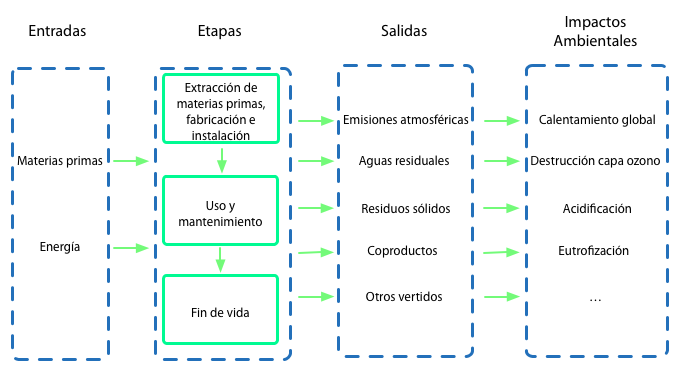
\includegraphics[width=15cm]{img/flujo_generico_acv.png}
\caption[Flujo genérico del ciclo de vida de un producto.]{Flujo genérico del ciclo de vida de un producto. Fuente: elaboración propia basada en \cite{pfullana}.}
\label{fig:flujo_generico_acv}
\end{figure}

\section{Impactos potenciales del adoquín al medio ambiente}
A la hora de analizar los aspecto medioambientales de un sistema es necesario establecer diferentes niveles de análisis para poder seleccionar una estrategia de estudio, ya que a lo largo de la vida de un producto se pueden encontrar diferentes contextos.

\begin{figure}[!htb]
\centering
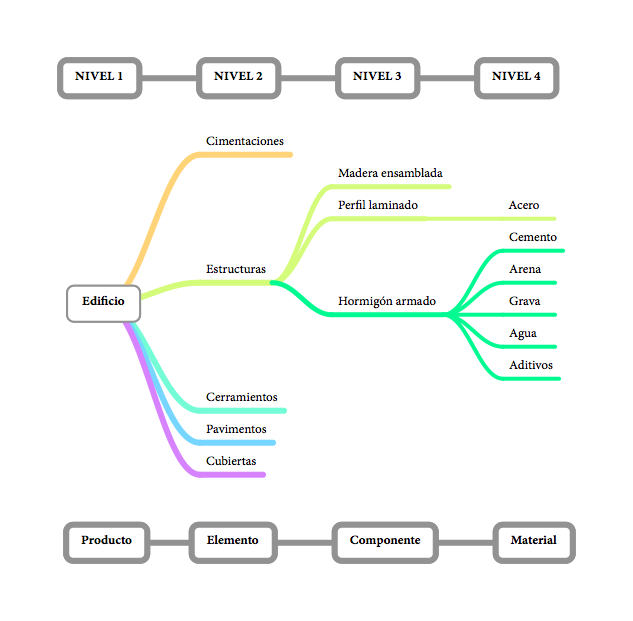
\includegraphics[width=15cm]{img/niveles_productos_construccion.png}
\caption[Niveles de los productos de la construcción.]{Niveles de los productos de la construcción. Fuente: elaboración propia basada en \protect\cite{carvalho}.}
\label{fig:niveles_productos_construccion}
\end{figure}

Al ser el adoquín un elemento de pavimentación se encontraría en el denominado nivel 2 (ver figura \ref{fig:niveles_productos_construccion}). Los impactos medioambientales del nivel 2 se clasifican según el momento de su vida en:

\begin{itemize}
  \item Extracción de materias primas, fabricación e instalación:
    \begin{itemize}
     \item Consumo de energía y recursos naturales en los procesos de extracción de materias primas, fabricación, instalación y transporte.
     \item Producción de ruidos y vibraciones.
     \item Producción de residuos por excedentes de procesos y embalajes.
     \item Emisiones de partículas al aire (p. ej.: polvo).
    \end{itemize}
  \item Uso y mantenimiento:
    \begin{itemize}
      \item Consumo de energía y recursos en los procesos de mantenimiento.
      \item Producción de residuos o sustancias tóxicas en función de los procesos de mantenimiento, su naturaleza y vida útil.
    \end{itemize}
  \item Fin de vida:
    \begin{itemize}
      \item Consumo de energía en el proceso de transporte y reciclaje.
      \item Producción de residuos por la parte no reciclada.
    \end{itemize}
\end{itemize}

\section{Prefabricados del cemento. Adoquines}

\subsection{Historia de los adoquines}
A lo largo de la historia de la humanidad se han ido utilizando diferentes tipos de adoquines para pavimentar los suelos urbanos. Los primeros adoquines eran de piedra, obtenidos a partir de los guijarros de río colocados sobre una capa de arena, usando una mezcla de cal y arena como sellante de juntas  \cite{euroadoquin}.

Debido al coste y el ruido del tráfico rodado, en la primera mitad del siglo XIX comenzaron a usarse los adoquines de madera, utilizando para el sellado residuos bituminosos. Su reducida duración y la posterior aparición de los neumáticos hicieron que los adoquines de madera fueran sustituidos por un modelo cerámico, con el que se usaba la misma arena tanto para la base como sellante.

Los adoquines de piedra iniciales seguían siendo más resistentes y además no eran tan deslizantes como los cerámicos. A finales del siglo XIX se fabricó por primera vez el \textbf{adoquín de hormigón}. Estos adoquines proporcionaban una mayor uniformidad que los de piedra, eran muy resistentes y con un coste inferior. Alemania y Países Bajos fueron los primeros en incorporar este nuevo formato de adoquín a sus núcleos urbanos. Al principio se usaban modelos que imitaban a los de piedra tanto en forma como colocación, pero pronto se añadieron formas dentadas o curvas, permitiendo una mejor alineación con el trazado.

Finalmente, durante la década de los 70 se mejoraron sustancialmente los sistemas de fabricación, permitiendo una gran variedad de modelos de adoquines y un abaratamiento de los costes de fabricación e instalación que llega hasta nuestros días.

\subsection{Ventajas e inconvenientes del uso de adoquines}\label{sec:ventajas}

En comparación con otros tipos de pavimentos tales como los asfálticos o los pavimentos contínuos hormigonados, los adoquines presentan las siguientes ventajas:

\begin{itemize}
\item Fabricación: no se utilizan derivados del petróleo, que suelen ser caros y contaminantes, además de requerir una mayor aportación de energía durante el proceso de fabricación. En contraposición, pueden utilizarse cementos y áridos locales, disminuyendo los costes de transporte.

El proceso de fabricación de los adoquines requiere una maquinaria específica debido a que son sometidos a presión y vibración para segurar una resistencia y durabilidad adecuadas. Esto implica un control sobre la fabricación, consistencia y fiabilidad del producto mayor que el resto de pavimentos.

\item Instalación: aunque los adoquines pueden colocarse de forma automatizada, están diseñados de base para ser colocados manualmente, permitiendo instalarse en zonas de difícil acceso, cargas elevadas (muelles de carga, aeropuertos, \ldots), resolver trazados complejos o pendientes pronunciadas. A diferencia de los pavimentos asfálticos, su ejecución no depende de la temperatura ambiente y pueden ser utilizados inmediatamente después de su finalización, lo que implica una reducción en los tiempos de ejecución de obra.

\item Comportamiento: los adoquines pueden ser diseñados para ser muy resistentes tanto a cargas verticales (distribuidas o puntuales) como a esfuerzos horizontales (aceleración-frenada, giros,\ldots). Además, soportan bien sin degradarse los vertidos de aceites y combustibles sobre el pavimento. Los niveles de ruido generados por el tráfico son similares o inferiores a otros pavimentos en ausencia de humedad y sensiblemente inferiores en condiciones de humedad, especialmente a bajas velocidades. La resistencia a deslizamiento es mayor al del resto de pavimentos.

\item Mantenimiento: la vida útil del adoquín viene determinada principalmente por el comportamiento de la base, subbase y explanada y no por el propio adoquín. La vida útil \footnote{La vida útil se considera como la duración estimada que un objeto puede tener cumpliendo correctamente con la funcion para la cual ha sido creado.} de cálculo suele ser a 30 años, aunque en condiciones normales puede superar los 50 años. De esta manera, al renovar el pavimento se puede reutilizar un 95\% de los adoquines originales \cite{euroadoquin}. El adoquín es la mejor opción en zonas donde aún no se han implantado todos los servicios de públicos debido a que pueden ser levantados fácilmente para llevar tareas de instalación o reparación en el subsuelo. La conservación de los adoquines se limita al relleno de juntas erosionadas con arena de sellado cada cierto tiempo y a la reposición de adoquines fracturados.

\item Costes: aunque inicialmente el precio del metro cuadrado instalado es algo superior a otros pavimentos, a largo plazo es mucho más barato debido al menor mantenimiento y la reutilización de piezas. Los pavimentos asfálticos y hormigonados requieren un mayor esfuerzo e inversión a la hora de ser reparados o retirados para acceder al subsuelo \cite{pavimentos,euroadoquin}.

\item Aspecto estético: actualmente los adoquines pueden diseñarse de todas formas, texturas, colores y disposiciones según las necesidades de la obra.
\end{itemize}


Realmente el uso de adoquines apenas tiene inconvenientes, aunque existen varios, entre los que destacan:

\begin{itemize}
  \item Incomodidad: debido a que el pavimento está lleno de juntas de separación entre adoquines y poco a poco se vuelve irregular, la circulación y el paso pueden ser incómodos y conllevar mayores costes de operación a los vehículos.
  \item Nieve: el pavimento de adoquines suele ser irregular y no permite bien la retirada de nieve en zonas con climas donde nieva mucho. Por otro lado, la nieve se derrite antes en pavimentos de asfalto, de color negro, debido al calentamiento del sol.
\end{itemize}

\section{Materias primas de los prefabricados del cemento}
Las características de las materias primas que se pueden emplear en la fabricación de los adoquines se contemplan en la norma UNE-EN 1338:2004/AC:2006 \cite{une1338}. En ella se especifican detalladamente los materiales, propiedades, requisitos y métodos de ensayo de los adoquines prefabricados de hormigón no armados y accesorios complementarios, previstos para uso peatonal, uso en áreas sometidas a tráfico de vehículos y cubiertas, como por ejemplo: aceras, límites de áreas, sendas para bicicletas, aparcamientos, carreteras, autopistas, áreas industriales, aeropuertos, estaciones de autobuses y gasolineras. Esta norma no trata la visibilidad y la tactibilidad de los adoquines ni los adoquines permeables.

\subsection{Cemento}
El cemento es un conglomerante formado a partir de arcilla y caliza (\ce{CaCO3}), que se endure al mezclarse con agua. Para producir cemento (ver figura \ref{fig:cemento}), la arcilla y la caliza se muelen juntas. A esta mezcla se le añade yeso para conferirle la propiedad de fraguar y endurecerse. El resultado se introduce en un horno rotatorio, normalmente seco por ser más eficiente energéticamente, a una temperatura aproximada de 1450\si{\celsius}. A continuación se introduce el material en un incinerador donde el calentamiento produce la liberación del \ce{CO2} de la caliza y se produce el cemento \emph{clinker}.

\begin{center}
\ce{CaCO3 + calor -> CaO + CO2}
\end{center}

El clinker es el óxido de calcio (\ce{CaO}) obtenido de la reacción anterior, que puede encontrarse acompañado de otros minerales como hierro, aluminio o silicio. El aporte de calor necesario para obtener el clinker representa la mayor parte del coste energético en la producción de cemento.

Por último, se produce la molienda del clinker junto con yeso y otros materiales (bauxita, arena,\ldots) para mejorar sus propiedades, produciendo el cemento.

\begin{figure}[!htb]
\centering
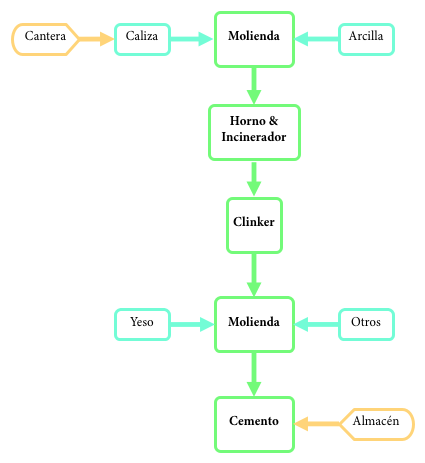
\includegraphics[height=10cm]{img/cemento.png}
\caption[Diagrama de flujo de la fabricación del cemento.]{Diagrama de flujo de la fabricación del cemento. Fuente: elaboración propia basada en \protect\cite{jsjunnesson}.}
\label{fig:cemento}
\end{figure}

Cuando se utiliza la palabra \emph{cemento} se refiere normalmente al cemento tipo Portland —supone un 95\% de la producción de cementos—, nombre no comercial que implica un proceso de producción y una composición característicos \cite{jsjunnesson}. De acuerdo a la norma UNE-EN 197-1:2011 \cite{une1971}, el cemento se divide en tres grupos en función de la cantidad de cemento Portland incluido: CEM I, CEM II y CEM III. El CEM I (95\% a 100\% de contenido de cemento Portland) es el más usado en la fabricación de adoquines.

Con respecto a la normativa específica de adoquines, la norma UNE 80301:1996 \cite{une80301} en el ámbito de España establece los requisitos que debe tener el cemento común. Si se utilizan cementos especiales se recurrirá a la norma UNE 80303:2013, y si son blancos a la norma UNE 80305:2012.

\subsection{Áridos}
Los áridos (entre los que se incluye la arena) son partículas de roca que pueden ser tanto gravas (piedras de forma natural) como macadán (piedras trituradas), teniendo cada tipo una textura diferente (figura \ref{fig:aridosnaturalesytriturados}). Se pueden añadir diferentes tamaños de áridos para ejercer una función específica según el tipo. Fracciones menores rellenarán las cavidades que haya entre partículas mayores, aportando adherencia a costa de un mayor peso.

\begin{figure}[!htb]
\centering
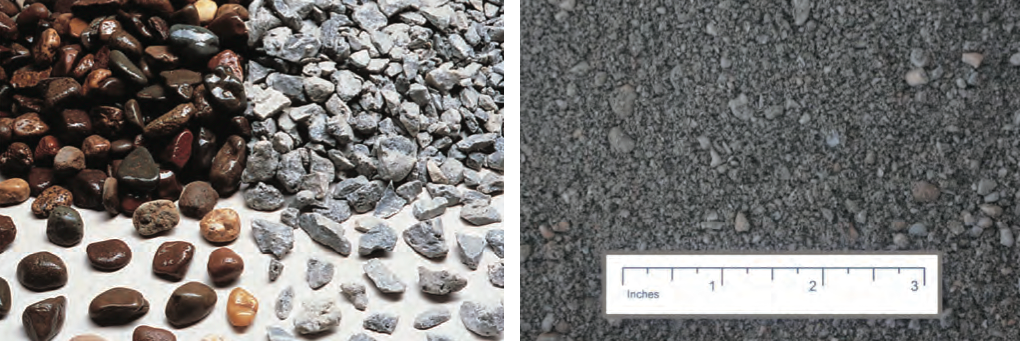
\includegraphics[width=13cm]{img/aridos.png}
\caption[Áridos naturales y triturados. Granulometrías.]{Áridos naturales y triturados. Granulometrías. Fuente: \cite{sustpave}.}
\label{fig:aridosnaturalesytriturados}
\end{figure}

El material de machaqueo para la producción de macadán se criba para eliminar las partículas menores. Debido a que las partículas que forman el macadán son más irregulares, es más fiable como material de relleno por su capacidad de incrustamiento (la grava tiene una forma más redondeada). El macadán puede ser utilizado de forma más generalizada en función de la localización ya que la grava natural es un recurso más limitado.

La fuente de recursos de áridos son principalmente de río, mina o cantera o piedras trituradas (macadán). La granulometría de los áridos que se utilicen deberá cumplir las características indicada en la norma UNE-EN 1338:2004/AC:2006 \cite{une1338}.

\subsection{Agua}
El agua es muy importante en la constitución del hormigón. Reacciona químicamente con el cemento —hidratación— para proporcionar las propiedades deseadas del hormigón \cite{nrmca}. El agua de amasado es la cantidad de agua que toma contacto con el cemento y se usa para determinar las proporciones del resto de elementos para formar la mezcla. La fuerza y la durabilidad del cemento viene dado en gran parte por la cantidad de agua.

Además de su cantidad, la calidad del agua utilizada tiene efectos importantes en las propiedades del hormigón fresco, tales como el tiempo de fraguado y la facilidad de trabajo. También tiene importancia en la fuerza y durabilidad del hormigón endurecido.

\subsubsection{Fuentes posibles de agua}

Por norma general el agua adecuada para el consumo humano —agua potable— es válida. No obstante, el agua no potable puede ser utilizada siempre que no tenga un impacto negativo en las propiedades del hormigón. La mayoría de las plantas tienen una fuente de agua municipal que proporciona agua potable sin necesidad de pruebas de calidad. En zonas rurales o en plantas portátiles in situ —instaladas y desinstaladas en el propio lugar del proyecto—, se suelen utilizar fuentes de agua no potable como ríos o masas de agua.

Otra fuente de agua es la reciclada de la limpieza —agua de lavado— de la mezcladora y otros elementos de la planta. También se podrá aprovechar el agua de precipitaciones atmosféricas que pueda recolectarse en las instalaciones de la planta.

El agua de procesado no sólo se genera de la fabricación del hormigón, sino también del lavado del hormigón reciclado. Los sistemas de recolección procesan el agua con el cemento y los áridos en forma de lechada que puede ser también utilizada como agua para la mezcla de hormigón.

Las normativas medioambientales suelen requerir que las plantas de fabricación traten y procesen tanto el agua de lluvia como el de procesado —agua de operaciones— para que adquiera ciertos niveles de pH y contenidos sólidos antes de que abandonen las instalaciones \cite{ermco}.

\subsubsection{Cualificación del agua no potable}
El agua es el recurso más importante para el ser humano. En algunas zonas el suministro de agua potable es muy escaso. El uso de fuentes de agua no potables para la producción de hormigón mantiene una producción sostenible de hormigón conservando los recursos de agua potable. La gestión del agua procedente de la producción de hormigón conforme con las normativas medioambientales representa un coste adicional para el fabricante, por lo que el uso de agua no potable representa un ahorro considerable en la producción de hormigón. Cuando se utilizan fuentes de agua no potable es importante verificar y documentar que las impurezas que contiene no merman las características del hormigón, ya que las fuentes pueden contener aceites, grasas, sales disueltas y otros elementos no controlados. Por esta razón, el fabricante debería tener en cuenta que su uso implica un coste adicional que evaluar y controlar.

\subsection{Aditivos}
Se podrán utilizar adiciones o aditivos siempre que produzcan el efecto deseado (acelerante, retardante,\ldots) y no afecte a las características esperadas del hormigón.

\section{Consideraciones de la instalación de pavimentos de adoquines}
La correcta colocación y mantenimiento del pavimento con adoquines es igual de importante que la calidad en los materiales y los procesos de fabricación \cite{euroadoquinc} para que el funcionamiento del pavimento sea el adecuado.

Hay múltiples manuales y guías técnicas que explican los criterios prácticos y recomendaciones para una correcta colocación de los adoquines.

La planificación del trabajo empieza estudiando el tipo de vía y uso principal al que estará destinado el pavimento. Una vez decidido es necesario preparar la explanada y las diferentes capas componentes en función de ese uso. A continuación se coloca la capa de adoquines, se sella con arena y se realiza un vibrado del pavimento. Por último se realiza una limpieza final.

\subsection{Capas componentes}

El pavimento de adoquines está compuesto por hasta un máximo de seis capas, cuyas dimensiones y composición dependerán del uso destinado de la vía:

\begin{itemize}
\item Explanada: terreno natural adecuadamente compactado hasta alcanzar una capacidad portante mínima.
\item Subbase: conjunto de capas naturales, de material granular seleccionado, estabilizado y compactado, situadas directamente sobre la explanada.
\item Base: principal elemento portante de la estructura, situada sobre la subbase. Puede ser realizada con material granular, zahorra artificial, con un mayor grado de compactación que el alcanzado en la subbase —base flexible—, o estar realizada con hormigón magro —base rígida.
\item Lecho de árido: base de apoyo de los adoquines, destinada a absorber sus diferencias de espesor debidas a la tolerancia de fabricación, de manera que estos una vez compactados formen una superficie homogénea.
\item Adoquines: elementos prefabricados de hormigón, cuya cara exterior, una vez colocados, forman la capa de rodadura de la superficie a pavimentar.
\item Relleno final: una vez encastrados en el lecho de árido, sus juntas precisan un relleno final para transferir a los elementos contiguos las cargas a las que sean sometidos por acción del tráfico.
\end{itemize}

\subsection{Determinación de la sección tipo}\label{sec:secciontipo}

Se consideran los siguientes casos:

\begin{enumerate}
\item Viales y zonas de aparcamiento\footnote{No suelen existir zonas peatonales puras. Siempre se contemplará el paso eventual de vehículos de mantenimiento, limpieza y servicios.}.
\item Zonas industriales.
\end{enumerate}

Para cada caso, viales o zonas industriales, la sección puede obtenerse de forma abreviada en función de dos variables:
\begin{itemize}
\item Tipo de explanadas.
\item Categoría de tráfico.
\end{itemize}

\subsubsection{Tipo de explanada}

Se utiliza un sistema de clasificación de su capacidad portante mediante el índice CBR (California Bearing Ratio), indicando el tanto por ciento de la presión ejercida por un pistón sobre el suelo para alcanzar una determinada penetración baremado según un juego de muestras normalizados (ver tabla \ref{indicecbr}).

\begin{table}[!htb]
\centering
\begin{tabular}{cc}
\toprule
Calidad de la explanada & Índice CBR\\
\midrule
E1 & 5 $\leq$ CBR = 10\\
E2 & 10 $\leq$ CBR = 20\\
E3 & 20 $\leq$ CBR\\
\bottomrule
\end{tabular}
\caption[Índice CBR.]{Índice CBR. Fuente: \protect\cite{euroadoquinc}.}
\label{indicecbr}
\end{table}


\subsubsection{Categoría de tráfico}

\begin{table}[!htb]
\centering
\begin{tabular}{cc}
\toprule
Tipo & Categoría de tráfico\\
\midrule
Viales y zonas de aparcamiento & C0 \ldots C4\\
Zonas industriales & A \ldots D\\
\bottomrule
\end{tabular}
\caption[Categoría de tráfico.]{Categoría de tráfico. Fuente: \protect\cite{euroadoquinc}.}
\label{categoriadetrafico}
\end{table}

Si en un área limitada existen diversos usos, a efectos de unificación se debería emplear para toda la zona la carga de cálculo más exigente.

\begin{table}[!htb]
\centering
\begin{tabular}{p{7cm}c}
\toprule
Uso previsto & Categoría de tráfico\\
\midrule
Arterias principales con gran afluencia de tráfico, paradas de bus, estaciones de servicio, etc. (50 a 149 v.p.d.) & C0\\
Arterias principales (25 a 49 v.p.d.) & C1\\
Calles comerciales con gran actividad (16 a 24 v.p.d.) & C2\\
Calles comerciales cone escasa actividad (15 v.p.d.) & C3\\
Áreas peatonales, calles residenciales & C4\\
\bottomrule
\end{tabular}
\caption[Categoría de tráfico en viales y zonas de aparcamiento.]{Categoría de tráfico en viales y zonas de aparcamiento. Fuente: \protect\cite{euroadoquinc}.}
\label{categoriadetraficoenviales}
\end{table}

\begin{table}[!htb]
\centering
\begin{tabular}{cccc}
\toprule
\multicolumn{2}{c}{Área} & Uso & Intensidad de uso\\
\midrule
\multirow{7}{*}{Comercial} & De operación & — & Alta\\
& \multirow{2}{*}{Almacenamiento} & Mercancia convencional & Media\\
& & Mercancía pesada & Alta\\
& Manipulación & — & Alta\\
& \multirow{3}{*}{Estacionamiento} & Vehículos pesados y ligeros & Media\\
& & Vehículos pesados exclusivamente & Alta\\
& & Semirremolques & Alta\\
\midrule
\multirow{3}{*}{Militar} & De operación & — & Alta\\
& \multirow{2}{*}{Almacenamiento} & Mercancia convencional & Media\\
& & Mercancía pesada y semirremolques & Alta\\
\midrule
\multirow{3}{*}{Pesquera} & Almacenamiento & — & Media\\
& Manipulación & — & Alta\\
& Clasificación y venta & — & Media\\
\midrule
\multirow{3}{*}{Industrial} & De operación & — & Alta\\
& \multirow{2}{*}{Almacenamiento} & Mercancia convencional & Media\\
& & Mercancía pesada & Alta\\
\bottomrule
\end{tabular}
\caption[Intensidades de uso en zonas industriales.]{Intensidades de uso en zonas industriales. Fuente: \protect\cite{euroadoquinc}.}
\label{categoriadetraficoenzonasindustrialesintensidades}
\end{table}

\begin{table}[!htb]
\centering
\begin{tabular}{cccc}
\toprule
Intensidad de uso & \multicolumn{3}{c}{Carga de cálculo}\\
\cmidrule{2-4}
& Alta & Media & Baja\\
\midrule
Elevada & A & B & C\\
Media & A & B & D\\
Reducida & B & C & D\\
\bottomrule
\end{tabular}
\caption[Categoría de tráfico en zonas industriales.]{Categoría de tráfico en zonas industriales. Fuente: \protect\cite{euroadoquinc}.}
\label{categoriadetraficoenzonasindustriales}
\end{table}

\subsection{Secciones tipo}

Las secciones tipo según la base y el uso previsto del área vistas en la sección \ref{sec:secciontipo} pueden resumirse en cinco tipos para cada tipo de base, granular (figura \ref{fig:seccionestipogranular}) u hormigón magro (figura \ref{fig:seccionestipohormigon}).

\begin{figure}[!htb]
\centering
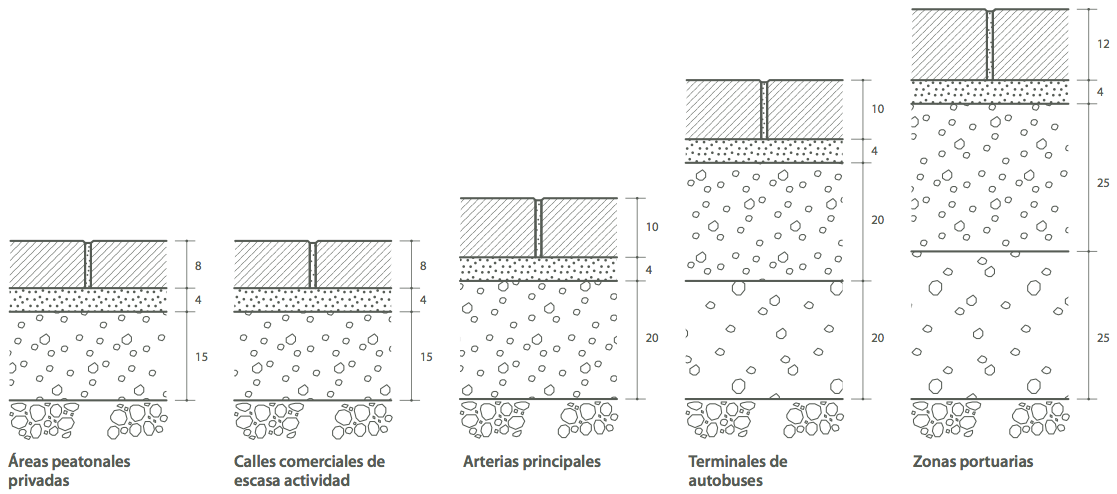
\includegraphics[width=15cm]{img/seccionestipo_1.png}
\caption[Secciones tipo para base granular.]{Secciones tipo para base granular. Unidades en cm. Fuente: \cite{fenollar}.}
\label{fig:seccionestipogranular}
\end{figure}

\begin{figure}[!htb]
\centering
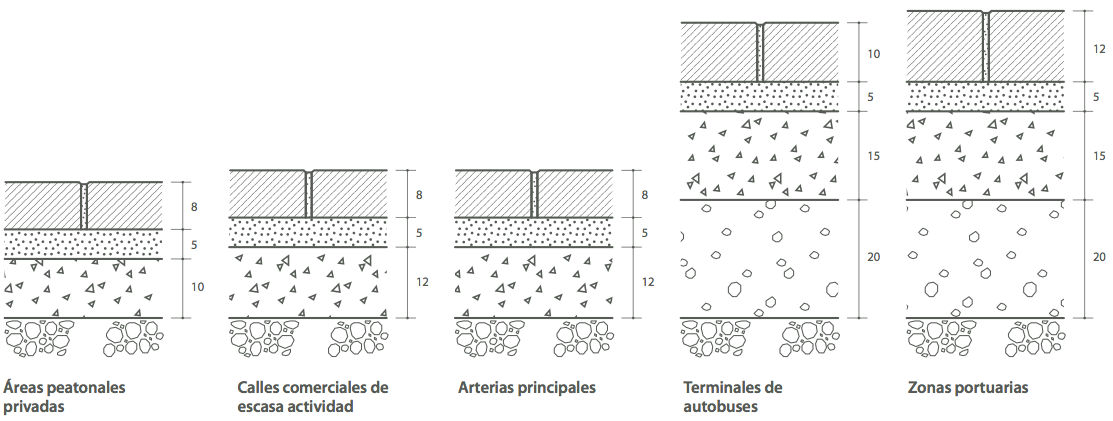
\includegraphics[width=15cm]{img/seccionestipo_2.png}
\caption[Secciones tipo para base de hormigón.]{Secciones tipo para base de hormigón. Unidades en cm. Fuente: \cite{fenollar}.}
\label{fig:seccionestipohormigon}
\end{figure}

\section{Consideraciones para el uso y mantenimiento de pavimentos de adoquines}\label{sec:consideracionesuso}

Una de las principales ventajas del pavimento con adoquines de hormigón es el fácil y económico mantenimiento del mismo durante su vida útil. Aunque la esperanza de vida de un adoquín está probada en 50 años, su tiempo de diseño es únicamente 30 años \cite{euroadoquin}.

Para que el funcionamiento del pavimento sea el correcto, las juntas deben permanecer llenas de arena —la presencia de pasto en las juntas no es nociva—. Si se pierde más de 1 \si{cm} de sello se recomienda corregir el hueco con arena de sellado.

Si se hunde el pavimento o es necesario acceder a infraestructura urbana, se deben retirar los adoquines, realizar la reparación y volver a reconstruir la franja de pavimento. La presencia de ondulaciones en la superficie del pavimento puede ser un indicio de que fue construido con una base mal construida o las características del tráfico no son las de diseño.

El pavimento de adoquines debe limpiarse, en principio, únicamente por barrido. El lavado con manguera debe ser poco frecuente y sólo cuando el tamaño de las juntas sea pequeño.

Existe un mantenimiento periódico, cada 3-5 años, que consiste en renovar el sellado del pavimento debido a la acción erosiva del medio ambiente \cite{malaka}.

\section{Consideraciones para el fin de vida del adoquín}\label{sec:consideracionesfindevida}

\subsection{Introducción}

La finalidad del reciclaje es conseguir un objetivo de cero residuos utilizando todos los materiales de subproductos encontrados en la rehabilitación o reconstrucción del pavimento. Esto no es sólo una ventaja económica, sino que el reciclaje local minimiza el impacto medioambiental reduciendo la huella de carbono, la energía utilizada y las emisiones, además de reducir la necesidad de vertederos y la extracción de materias primas no renovables.

El concepto del reciclaje debe verse como un proceso de ``cuna a cuna'' en contraposición al pensamiento de ``la cuna a la tumba'' de hace unos años. En la práctica no hay una tumba para los materiales utilizados en las infraestructuras sostenibles actuales, tan sólo un nuevo inicio que permite la aplicación de tecnologías para lograr la meta de cero residuos en la rehabilitación y reconstrucción de pavimentos de adoquines.

Mientras que en el pasado los costes económicos eran el factor prioritario que empujaban al reciclaje, actualmente se tienen en cuenta los recursos limitados y la conciencia medioambiental en beneficio de la sostenibilidad en el proceso. Aunque el coste económico sigue siendo un factor importante, la concienciación política y social de la necesidad de ser sostenible ha aumentado considerablemente en los últimos años \cite{sustpave}. Los beneficios del reciclaje incluyen:

\begin{itemize}
  \item ahorros económicos.
  \item menor uso de materias primas no renovables.
  \item menor demanda de combustibles y emisiones asociadas del transporte de desechos a vertederos o de nuevos materiales a su destino.
  \item mejora del uso del suelo municipal, minimizando tanto la necesidad de vertederos como de nuevos espacios para la extracción de recursos.
\end{itemize}

Se generan aproximadamente 200 millones de toneladas de Residuos de la Construcción y Demolición (RCDs) al año en Europa. El hormigón es un material de construcción excelente para edificios energéticamente eficientes y duraderos. Por suerte, además puede reciclarse con un impacto medioambiental mínimo \cite{europeanconcrete}.

\subsection{Reciclado del hormigón}

En la actualidad, el hormigón —cemento, áridos, arena y agua— recuperado de los RCDs no puede utilizarse para obtener de nuevo cemento. En su lugar, ese hormigón puede ser machacado y utilizado como árido para formar parte de nuevas estructuras, principalmente formando bases de carreteras, aunque cada vez más nuevo hormigón usando un porcentaje de hormigón reciclado. Se puede utilizar árido reciclado hasta un máximo de un 20\% del total necesario en la fabricación de nuevo hormigón conservando las propiedades originales \cite{europeanconcrete}.

El hormigón machacado se utiliza principalmente en obras de construcción, carreteras, calles y aparcamientos, aunque también como relleno de excavaciones de tuberías y cimientos de edificios. El hormigón reciclado en forma de árido reciclado tiene frecuentemente mejor grado de compacidad y densidad y es normalmente más barato que el material original \cite{jsjunnesson}.

El proceso de reciclado suele consistir en que el RCD llega a la planta de reciclaje, donde es introducido en una tolva de recepción, protegida con una reja de filtrado para la eliminación de los materiales de gran tamaño. El residuo es conducido por un sistema de cintas para su clasificación y triaje. Finalmente se produce un machacado seguido de un lavado-secado y un tamizado \cite{monografia} \cite{gerd}.

En el caso concreto de los adoquines, su fin de vida se puede desglosar en dos escenarios \cite{euroadoquin}:
\begin{itemize}
  \item el 95\% de los adoquines son recuperados para su reciclaje;
  \item el 5\% son desechados en vertederos junto con otros residuos.
\end{itemize}

El reciclado puede tratarse como un beneficio para el medio ambiente, debido a que se evita extraer nuevas materias primas. Ese beneficio se obtiene como la diferencia entre los impactos de las nuevas materias primas y los impactos del proceso de reciclaje.

El reciclado del hormigón en nuevos áridos implica que habrá un \textbf{producto evitado}, que ya no es necesario fabricar, que será el propio árido. que además será coincidente con el \textbf{producto secundario}, que es el obtenido después del proceso de reciclaje.

\section{Origen del estudio}
Malaka de Prefabricados es una empresa malagueña que inició su actividad en 1994. Su compromiso consistía en integrarse en el tejido industrial de la provincia, estableciendo lazos con otras industrias locales, y apostar por un producto de calidad que marcara la diferencia en el mercado sin repercutir en el precio.

\begin{figure}[!htb]
\centering
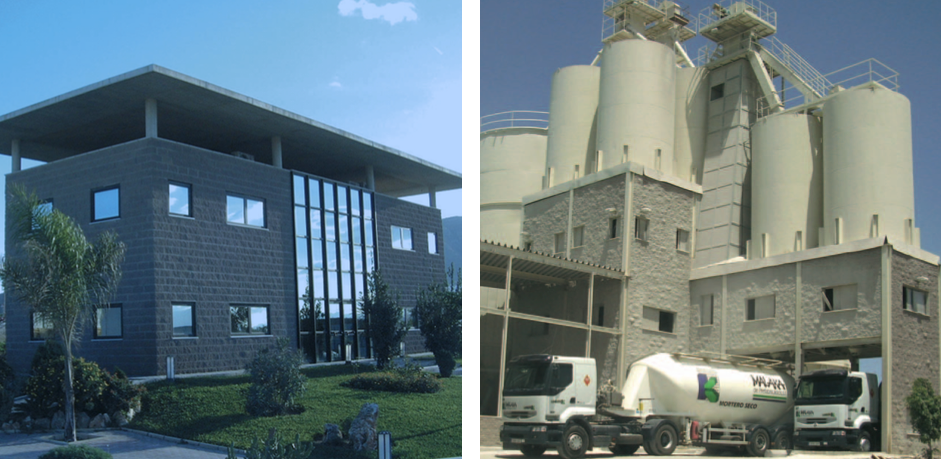
\includegraphics[width=15cm]{img/malaka1.png}
\caption[Instalaciones de Malaka de Prefabricados.]{Instalaciones de Malaka de Prefabricados. Fuente: \protect\cite{malakacatalogo}.}
\label{fig:malakainstalaciones1}
\end{figure}

A finales de la década de los 90 y principios del nuevo milenio experimentaron un fuerte crecimiento como consecuencia del rápido auge del sector de la construcción en Andalucía, convirtiéndose en un referente de los prefabricados en la provincia y en la comunidad autónoma.

Sus principales líneas de producción son los adoquines, bloques y bordillos de hormigón, a los que se dedica por completo una planta de producción automatizada. La línea de adoquines dispone de varias gamas de producto debido a la versatilidad y demanda de la que disfruta. El resto de productos —tubos, registros, aligerantes, casetones y mortero seco ensilado— se fabrican en la segunda planta.

\begin{figure}[!htb]
\centering
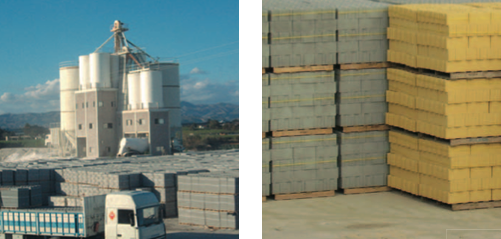
\includegraphics[width=15cm]{img/malaka2.png}
\caption[Instalaciones accesorias de Malaka de Prefabricados.]{Instalaciones accesorias de Malaka de Prefabricados. Fuente: \protect\cite{malakacatalogo}.}
\label{fig:malakainstalaciones2}
\end{figure}

El compromiso de calidad en sus productos pasó por cumplir todos los requisitos de la normativa española y europea, adoptando el marcado CE como sello de calidad. Tanto clientes como partners pueden dar muestra de su confianza en la calidad de los mismos. Entre sus principales proyectos se encuentran el Palacio de Deportes Martín Carpena (Ferrovial-Agroman), el Parque Temático de Melilla (Dragados) y colaboraciones con los ayuntamientos de Marbella y Estepona.

Durante los casi veinte años en la industria han intentado adoptar las mejores y más novedosas tecnologías de fabricación del sector, ampliando de forma progresiva el tamaño de sus instalaciones en la Finca Pizarro, a las afueras de la ciudad de Málaga.

La empresa adoptó a principios de 2000 la Certificación de Sistemas de Gestión de la Calidad (ISO 9001) y varios años más tarde la Certificación Sistemas de Gestión Ambiental (ISO 14000) como referente de compromiso con la calidad de su producción y con el medioambiente.

%!TEX root = informe.tex
\chapter{Normas y referencias}
\section{Disposiciones legales y normas aplicadas}

Para la realización de este proyecto se han tenido en cuenta la siguiente normativa:

\begin{itemize}
  \item UNE-EN-ISO 14040:2006, Gestión Ambiental. Análisis de ciclo de vida. Principios y marco de referencia.
  \item UNE-EN-ISO 14440:2006, Gestion Ambiental. Análisis de ciclo de vida. Requisitos y directrices.
  \item UNE-EN-ISO 150041EX:1998, Análisis de ciclo de vida simplificado.
  \item UNE-EN-ISO 14006:2011, Sistemas de gestión ambiental. Directrices para la incorporación del ecodiseño.
  \item UNE-EN 1338:2004/AC:2006 Adoquines de hormigón. Especificaciones y métodos de ensayo.
  \item UNE-EN 197-1:2011 La norma europea de especificaciones de cementos comunes.
  \item UNE 80301:1996 Cementos. Cementos comunes. Composicion, especificaciones y criterios de conformidad.
  \item UNE 127338:2007 Propiedades y condiciones de suministro y recepción de los adoquines de hormigón. Complemento nacional a la Norma UNE EN 1338.
  \item UNE-CEN/TR 15941:2011 IN Sostenibilidad en la construcción. Declaraciones ambientales de producto. Metodología para la selección y uso de datos genéricos.
  \item UNE-EN15804:2012 Sostenibilidad en la construcción.Declaracionesambientales de producto.
  \item UNE-EN 15978:2012 Sostenibilidad en la construcción. Evaluación del comportamiento ambiental de los edificios. Métodos de cálculo.
  \item ISO. UNE-ISO 21930 Sostenibilidad en la construcción de edificios. Declaración ambiental de productos de construcción.
\end{itemize}

\bibliographystyle{plain}
\bibliography{informe}

\section{Programas de cálculo}

El software de Análisis de Ciclo de Vida elegido es SimaPro de PRé Consultants.

Los cálculos se han realizado mediante la aplicación de hoja de cálculo Apple Numbers.app.

\section{Plan de gestión de la calidad aplicado durante la redacción del Proyecto}

Para la realización de este proyecto se ha aplicado la siguiente normativa:
\begin{itemize}
  \item UNE 157001:2002 Criterios generales para la elaboración de proyectos.
  \item UNE 50132:1994 Documentación. Numeración de las divisiones y subdivisiones en los documentos escritos.
  \item UNE 1027:1995 Dibujos técnicos. Plegado de planos.
  \item UNE 1032:1982 Dibujos técnicos. Principios generales de representación.
  \item UNE 1035:1995 Dibujos técnicos. Cuadro de rotulación.
  \item UNE 1039:1994 Dibujos técnicos. Acotación. Principios generales, definiciones, métodos de ejecución e indicaciones especiales.
\end{itemize}

Durante la redacción de este proyecto se han corroborado los datos aportados por el fabricante. Se han revisado errores de transcripción de datos, fallos en los cálculos, así como errores gramaticales y ortográficos. Además, se ha comprobado la consistencia de los conceptos de estudio con la metodología empleada. Por último, se ha utilizado un sistema de copia de seguridad basada en control de versiones, por la cual los datos pueden ser recuperados o consultados en cualquier momento.

%!TEX root = informe.tex
\chapter{Definiciones y abreviaturas}
\begin{itemize}
  \item AENOR (Asociación Española de Normalización y Certificación): entidad de certificación de sistemas de gestión, productos y servicios, y responsable del desarrollo y difusión de las normas UNE.
  \item Análisis del Ciclo de Vida (ACV): recopilación y evaluación de las entradas, las salidas y los impactos ambientales potenciales de un sistema del producto a través de su ciclo de vida.
  \item Análisis del Inventario del Ciclo de Vida (ICV): fase del análisis del ciclo de vida que implica la recopilación y la cuantificación de entradas y salidas para un sistema del producto a través de su ciclo de vida.
  \item Aspecto ambiental: elemento de las actividades, productos o servicios de una organización que puede interactuar con el medio ambiente.
  \item BUWAL: Bundesamt für Unwelt, Wald und Landshaft. Oficina Federal de Medio Ambiente, Bosque y Campo (Suiza).
  \item Categoría de impacto: clase que representa asuntos ambientales de interés a la cual se pueden asignar los resultados del análisis del inventario del ciclo de vida.
  \item CEN: Comité Europeo de Normalización.
  \item Ciclo de vida: etapas consecutivas e interrelacionadas de un sistema del producto, desde la adquisición de materia prima o de su generación a partir de recursos naturales hasta la disposición final.
  \item De la cuna a la tumba: expresión que referencia al ciclo de vida de un producto desde la extracción de las materias primas hasta la disposición.
  \item Eco-Indicador: indicador ambiental, desarrollado por PRé Consultants para el gobierno de Holanda.
  \item Ecodiseño: diseño que considera acciones orientadas a la mejora ambiental del producto o servicio en todas las etapas de su ciclo de vida, desde su creación en la etapa conceptual, hasta su tratamiento como residuo.
  \item Emisiones atmosféricas: introducción en la atmósfera por el hombre, de forma directa o indirecta, de sustancias o energía que tengan una acción perjudicial para la salud humana o el medio ambiente.
  \item Evaluación del Impacto del Ciclo de Vida (EICV): fase del análisis del ciclo de vida en la que los hallazgos del análisis del inventario o de la evaluación del impacto, o de ambos, se evalúan en relación con el objetivo.
  \item Impacto ambiental: alteración apreciable sobre la salud y bienestar de cualquier ser vivo o sobre el medio ambiente. En relación al ACV, se trata de la anticipación razonable a un efecto.
  \item ISO (International Standard Organitation). Organización Internacional de Estándares.
  \item Life Cycle Assessment (LCA): acrónimo en inglés de Análisis de Ciclo de Vida.
  \item Límite del sistema: conjunto de criterios que especifican cuales de los procesos unitarios son parte de un sistema del producto.
  \item Medio ambiente: conjunto de factores físico-químicos (agua, aire, clima, etc.), biológicos (fauna, flora y suelo) y socioculturales (asentamiento y actividad humana, uso y disfrute del territorio, formas de vida, etc.) que integran el entorno en que se desarrolla la vida del hombre y la sociedad (RD 4/1986 de 23 de enero 1986).
  \item Proceso unitario: elemento más pequeño considerado en el análisis del inventario del ciclo de vida para el cual se cuantifican datos de entrada y salida.
  \item Producto evitado: aquel material o producto que no es necesario generar debido a que ya se ha obtenido durante los procesos de otro producto.
  \item UNE: Una Norma Española.
  \item UNE-EN: Una Norma Española que además es Norma Europea (European Norm) a través del CEN.
  \item UNE-EN-ISO: Adaptación de normativa ISO a ámbito europeo por el CEN y de ahí al ámbito español por AENOR.
  \item Unidad funcional: aquella prestación o función que realiza un producto que permite su comparación con otros.
  \item Vida útil: duración estimada que un objeto puede tener cumpliendo correctamente con la función para la cual ha sido creado.
\end{itemize}

%!TEX root = informe.tex
\chapter{Metodología del Análisis de Ciclo de Vida}
\section{Introducción}

Como se ha mencionado en la sección \ref{sec:introantecedentes}, el Análisis de Ciclo de Vida de un producto incluye todos los procesos de producción y servicios relacionados con el producto durante su ciclo de vida completo, desde la extracción de las materias primas hasta su reciclaje y/o disposición final, pasando por la fabricación y los subproductos que lo forman, la instalación, el uso y mantenimiento del producto. También se pueden incluir en las diferentes etapas del ciclo de vida el almacenamiento, venta, transporte y otras actividades que se consideren relevantes. Si se incluyen todos las etapas anteriores, le denomina comúnmente Análisis de Ciclo de Vida ``de la cuna a la tumba''. Cuando únicamente se contempla desde que se obtienen las materias primas hasta que el producto se pone en el mercado, se le denomina ``de la cuna a la puerta''. Hay un enfoque más reciente basado en tener en cuenta que las salidas del Fin de Vida del sistema como materias primas del mismo sistema o de otro nuevo, al que se le denomina ``de la cuna a la cuna''.


El Análisis de Ciclo de Vida hace distinción entre ``Entradas'' —materias primas, energía— y ``Salidas'' —emisiones a la tierra, mar o aire, desechos y subproductos—, como refleja la figura \ref{fig:escenariolca}.

\begin{figure}[!htb]
\centering
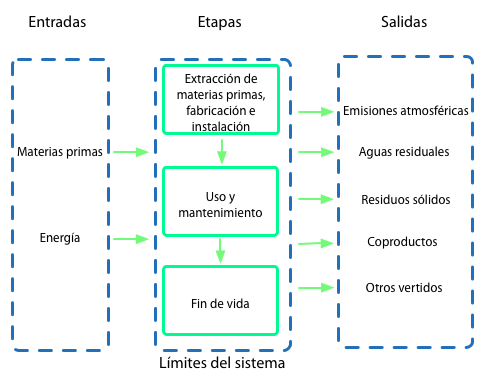
\includegraphics[width=12cm]{img/escenariolca.png}
\caption[Escenario de un ACV]{Escenario de un ACV. Fuente: basado en \protect\cite{epa}.}
\label{fig:escenariolca}
\end{figure}

En las ``Entradas'' también pueden aparecer productos que proceden de la \textbf{tecnoesfera} —productos no naturales—, que añadirán su historial medioambiental a los cálculos del producto y/o servicio. Para el caso de residuos, se tendrán que incluir los futuros procesos de tratamiento.

El Análisis de Impacto del Ciclo de Vida (AICV) recoge la totalidad de entradas y salidas a la naturaleza para realizar un estudio potencial de los efectos medioambientales relacionados con el producto \cite{iso14040}.

\subsection{Etapas del Análisis de Ciclo de Vida}\label{sec:etapaslca}

Según la norma UNE-EN-ISO 14040:2006, el estudio de Análisis de Ciclo de Vida se compone de cuatro fases, relacionadas según la figura \ref{fig:etapaslca}.

\begin{figure}[!htb]
\centering
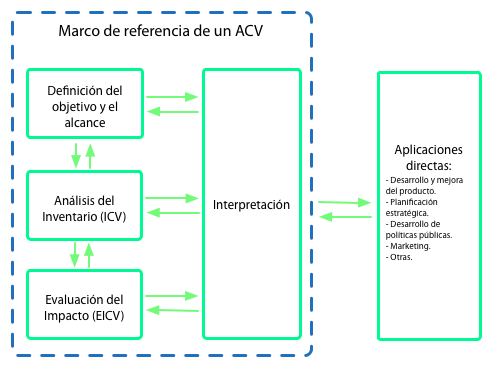
\includegraphics[width=12cm]{img/etapas_lca.png}
\caption[Etapas del Análisis de Ciclo de Vida.]{Etapas del Análisis de Ciclo de Vida. Fuente: \protect\cite{iso14040}.}
\label{fig:etapaslca}
\end{figure}

\subsubsection{Fase de definición de objetivos y alcance}
En esta fase se define el objetivo y el uso previsto del estudio, al mismo tiempo que el alcance de acuerdo con los límites del sistema, la unidad funcional y los flujos dentro del ciclo de vida, la calidad exigida a los datos, y los parámetros tecnológicos y de evaluación \cite{iso14040,ihobeeco}.

\subsubsection{Fase de Análisis de Inventario (ICV)}
En esta fase se recogen los datos correspondientes a las entradas materias primas, energía— y salidas —emisiones a la tierra, mar o aire, desechos y subproductos— para todos los procesos del sistema de producto. Durante esta fase es necesario definir completamente el ciclo de vida del producto.

La realización del ICV es un proceso iterativo. A medida que se recopilan los datos y se aprende más sobre el sistema, se pueden identificar nuevos requisitos o limitaciones, que requieran cambios en los procedimientos de recopilación de datos \cite{iso14040,ihobeeco}.

\subsubsection{Fase de Evaluación del Impacto Ambiental (EICV)}
En esta fase el inventario con las entradas y salidas es traspasado a indicadores de impactos ambientales potenciales al medio ambiente, a la salud humana y a la disponibilidad de recursos naturales \cite{iso14040,ihobeeco}.

Es la fase del ACV dirigida a conocer y evaluar la magnitud y la significancia de los impactos ambientales potenciales de un sistema. Se emplea un método de evaluación para transformar los datos recogidos en el ICV en resultados de carácter ambiental.

El EICV según la norma UNE-EN-ISO 14040:2006 \cite{iso14040} tiene tres categorías obligatorias:

\begin{itemize}
  \item Selección de categorías de impacto, indicadores de categoría y modelo de caracterización: estas categorías representan los impactos ambientales de interés a los cuales se quieren asignar los resultados del EICV. Existen múltiples categorías de impacto ambiental y su elección depende del objetivo del estudio, público al que va dirigido y el nivel de exactitud de los resultados requeridos. Las principales categorías de impacto contempladas por la SETAC 1\footnote{SETAC 1: Sociedad de Toxicología y Química Ambiental creada en 1979} (desarrollados en la sección \ref{sec:impactosamb}) son: calentamiento global, consumo de recursos energéticos, reducción de la capa de ozono, eutrofización, acidificación, consumo de materias primas y formación de oxidantes fotoquímicos.
  \item Asignación de resultados del ICV (clasificación): se asignan los datos del ICV a las categorías de impacto. Si una sustancia contribuye a varias categorías de impacto, tiene que ser considerada en todas esas categorías.
  \item Cálculo de resultados del indicador de categoría (caracterización): una vez asignadas todas las sustancias del ICV a sus categorías de impacto ambiental (clasificación), se compara su valor con respecto a la sustancia de referencia de dicha categoría. Esto se realiza mediante los factores de caracterización de cada sustancia, que representan la contribución de una sustancia a una determinada categoría de impacto en relación a la sustancia de referencia en dicha categoría. Cada sustancia se multiplica por su correspondiente factor de caracterización para obtener valores con unidades equivalentes, que pueden sumarse posteriormente para medir la contribución de las sustancias a esa categoría de impacto.
\end{itemize}

Además de las etapas obligatorias anteriores, existen otras opcionales que pueden utilizarse dependiendo del objetivo y alcance previsto:

\begin{itemize}
  \item Normalización: conversión de los resultados de la caracterización a unidades globales neutras, dividiendo cada uno por un factor de normalización. Mediante estos factores se representa el grado de contribución de cada categoría de impacto ambiental sobre el problema medioambiental local.
  \item Agrupación: clasificación de las categorías de impacto en otros grupos que engloben categorías de impacto con efectos similares.
  \item Ponderación: conversión de los resultados de los valores caracterizados (o normalizados) a una unidad común y sumable, multiplicándolos por su factor de ponderación. Pueden sumarse posteriormente spara obtener una puntuación total del impacto ambiental del sistema.
\end{itemize}

\subsubsection{Fase interpretación}
Es la fase del ACV en la que los resultados del ICV y el EICV son interpretados de acuerdo al objetivo y alcance marcados inicialmente. En esta fase se realiza un análisis de los resultados y se marcan las conclusiones.

\subsection{Impactos ambientales en el ciclo de vida}\label{sec:impactosamb}

Se define el \textit{Impacto ambiental} como cualquier cambio en el medio ambiente, adverso (negativo) o beneficioso (positivo), resultante en todo o en parte de las actividades, productos o servicios de una organización \cite{mlgceballos}.

Según la SETAC 1, se pueden diferenciar los siguientes tipos de impacto \cite{ihobeeco}:

\begin{itemize}
  \item Calentamiento global: fenómeno observado en las medidas de la temperatura que muestra en promedio un aumento en la temperatura de la atmósfera terrestre y de los océanos en las últimas décadas
  \item Consumo de recursos energéticos: energía consumida en la obtención de las materias primas, fabricación, distribución, uso y fin de vida del elemento analizado.
  \item Reducción de la capa de ozono: ffectos negativos sobre la capacidad de protección frente a las radiaciones ultravioletas solares de la capa de ozono atmosférica.
  \item Eutrofización: crecimiento excesivo de la población de algas originado por el enriquecimiento artificial de las aguas de ríos y embalses como consecuencia del empleo masivo de fertilizantes y detergentes que provoca un alto consumo del oxigeno del agua.
  \item Acidificación: pérdida de la capacidad neutralizante del suelo y del agua, como consecuencia del retorno a la superficie de la tierra, en forma de ácidos, de los óxidos de azufre y nitrógeno descargados a la atmósfera
  \item Consumo de materias primas: consumo de materiales extraídos de la naturaleza.
  \item Formación de oxidantes fotoquímicos: formación de los precursores que dan lugar a la contaminación fotoquímica. La luz solar incide sobre dichos precursores, provocando la formación de una serie de compuestos conocidos como oxidantes fotoquímicos (el ozono-\ce{O3} es el más importante por su abundancia y toxicidad).
\end{itemize}

\subsection{Ventajas e inconvenientes del ACV}

El Análisis de Ciclo de Vida es una herramienta que ofrece muchas ventajas:
\begin{itemize}
  \item el ACV es la única herramienta que examina los impactos medioambientales de un producto y/o servicio a través de su ciclo de vida.
  \item el ACV es un método estándar ISO, en referencia a las normas UNE-EN-ISO 14040:2006 y UNE-EN-ISO 14044:2006.
  \item el ACV proporciona una visualización fácil de entender de separando en etapas las fuentes de impacto.
  \item el ACV puede tanto guiar las decisiones de un fabricante (nivel microeconómico) como ayudar a un gobierno a definir una política de actuación (nivel macroeconómico).
  \item el ACV distingue entre la información relevante mediante cuantificación objetiva y los asuntos que pertenecen a políticas y elecciones sociales.
\end{itemize}

Por otro lado, el Análisis de Ciclo de Vida tiene ciertas limitaciones:
\begin{itemize}
  \item los resultados son geográficamente dependientes. Los resultados de un estudio en Europa no son aplicable en Estados Unidos sin tener en cuenta las variaciones geográficas correspondientes (por ejemplo, el mix eléctrico).
  \item el ACV sólo evalúa los impactos potenciales, no los verdaderos impactos, por lo que no proporciona ninguna información de las consecuencias.
  \item los resultados de dos ACVs para un mismo objeto de estudio puede diferir según los objetivos, procesos, calidad de los datos y el método de análisis de impacto utilizados. La ISO insiste en transparencia a la hora de realizar un ACV.
  \item un ACV detallado requiere un inventario de todos los procesos elementales incluidos dentro de los parámetros del sistema.
  \item se requiere el uso de bases de datos, software especializado y personas capacitadas para poder analizar los datos.
\end{itemize}

\section{Métodos de análisis de aspectos ambientales de productos y establecimiento de prioridades}

Existen varios métodos —cualitativos y cuantitativos— para analizar el perfil ambiental de un producto y establecer prioridades ambientales. Todos ellos se basan en el Análisis del Ciclo de Vida, lo que significa que analizan todas las fases del ciclo de vida del producto en cuanto a los aspectos ambientales del producto en cada una.

Los objetivos de estos métodos son:
\begin{itemize}
  \item Obtener una perspectiva general de los principales aspectos ambientales del producto durante todo su Ciclo de Vida.
  \item Identificar las prioridades ambientales.
\end{itemize}

A continuación se analizarán brevemente algunos de los métodos más interesantes: Matriz MET, Eco-indicadores y el software de Análisis de Ciclo de Vida. Éste último, debido a su importancia actual y a que son el método utilizado en este proyecto, será desarrollado con mayor amplitud en la sección \ref{sec:software}.

\subsection{Matriz MET}

La Matriz MET (Materiales/Energía/Toxinas) es una método cuantitativo y cualitativo con el que se obtiene una visión global de las entrada y salidas de cada etapa del Ciclo de Vida del producto. Es cuantitivo porque maneja cantidades, pero también se trata de un método cualitativo porque prioriza los aspectos ambientales y se basa en conocimientos ambientales y reglas de oro y no en cifras o resultados \cite{ihobeeco}.

La Matriz MET engloba:
\begin{itemize}
  \item M: utilización de Materiales en cada etapa del ciclo de vida. Incluye todas las entradas (consumos) de cada una de las etapas del ciclo de vida, proporcionando una visión de cuáles son las prioritarias por su mayor cantidad, toxicidad o por ser materiales escasos.
  \item E: utilización de Energía. Engloba el impacto de los procesos y transportes en cada una de las etapas del ciclo de vida —principalmente aquellos que consumen mucha energía—, proporcionando una visión de cuáles son los procesos o transportes de mayor impacto.
  \item T: emisiones Tóxicas. Recoge todas las salidas producidas en el proceso —emisiones, vertidos o residuos tóxicos—, proporcionando las salidas más importantes por su toxicidad.
\end{itemize}

El uso de la Matriz MET se recomienda:
\begin{itemize}
  \item Para recopilar datos antes de utilizar los Eco-indicadores o software de Análisis de Ciclo de Vida, ya que permite organizar la información de cada etapa del ciclo de vida.
  \item Para obtener una visión global rápida de las prioridades ambientales sin la necesidad de gran precisión.
  \item Como método alternativo cuando no existan Eco-indicadores relevantes para los materiales o los procesos del producto.
\end{itemize}

\subsection{Eco-indicadores}

El Eco-indicador es una método cuantitativa de fácil manejo. Es más preciso que la Matriz MET a la hora de priorizar los principales aspectos ambientales del producto en su ciclo de vida. Es un método cuantitativo porque la priorización se basa en cálculos numéricos \cite{ihobeeco}.

Los Eco-indicadores son el resultado de un proyecto desarrollado por un equipo multidisciplinar formado por industrias punteras de diferentes sectores, científicos de centros de investigación independientes y el gobierno holandés con el objetivo de intentar conseguir evaluar el impacto ambiental que ejerce la actividad industrial sobre el medio ambiente, centrándose en el impacto sobre el ecosistema, los recursos y la salud humana a nivel europeo. Los impactos tenidos en cuenta son: el efecto invernadero, la reducción de la capa de ozono, la lluvia ácida, la disminución de los recursos naturales, la disminución de la biodiversidad y el smog fotoquímico.

Existen diversos métodos basados en Eco-indicadores, entre los que cabe destacar \cite{mlgceballos}:

\begin{itemize}
  \item CML 2001: desarrollado en los Países Bajos, basado en su versión de 1992. El paso de normalización es opcional para ACVs simplificados, pero obligatorio para los exhaustivos. Las categorías de impacto ambiental son: agotamiento de los recursos abióticos, cambio climático, destrucción de capa de ozono, toxicidad humana, ecotoxicidad, smog fotoquímico, acidificación, eutrofización y uso de recursos.
  \item ReCiPe: del mismo equipo que la metodología EICV (ver sección \ref{sec:recipe}). Las categorías de impacto ambiental son: destrucción de capa de ozono, toxicidad humana, radiación, smog fotoquímico, formación de partículas, cambio climático, ecotoxicidad del suelo, acidificación del suelo, ocupación del suelo rural, ocupación de suelo urbano, transformación suelo natural, ecotoxicidad marina, eutrofización marina y agua dulce, ecotoxicidad de agua dulce.
  \item Ecoindicator 95: desarrollado por PRè Consultants, se basa en la existencia de una correlación entre la gravedad del efecto produccido por las emisiones y la distancia entre el nivel actual de emisiones y un nivel objetivo marcado como estándar de calidad ambiental, según un modelo de distancias al nivel objetivo.
  \item Ecoindicator 99: considera tres categorías de daños, relacionadas directamente con el resultado del inventario: salud humana, calidad del ecosistema y agotamiento de recursos. El Ecoindicador 95 es más un indicador de emisiones mientras que el Ecoindicador 99 lo es más de combustibles fósiles.
  \item EcoPoint: desarrollado por el Ministerio de Medioambiente de Suiza (BUWAL) en 1990, actualizado en 1997. Se basa en la distancia al objetivo que ofrece como resultado un indicador de impacto único.
  \item EPS: desarrollado por el Instituto de Investigación Medioambiental de Suecia en 1991. Se basa en una valoración de economía ambiental, es decir, determinar el daño y su asignación monetaria, en unidades ELU (Environmental Load Unit).
\end{itemize}

\section{Software de Análisis de Ciclo de Vida}\label{sec:software}

El mercado ofrece una amplia gama de programas para el Análisis de Ciclo de Vida que ofrecen diferentes tipos de prestaciones y rangos de precios. Entre ellos cabe destacar:

\begin{itemize}
  \item SimaPro: ver sección \ref{sec:simapro}.
  \item Gabi: permite esbozar ideas en su interfaz y ofrece un potente asistencia para la creación del inventario. Incorpora una base de datos propietaria que también funciona con \textit{ecoinvent}. Es compatible con los estándares UNE-EN-ISO 14040:2006 y bastante flexible.
  \item Quantis Suite: facilita el acceso a personas no expertas con plantillas y asistentes. Incorpora una base de datos propia.
  \item EarthSmart: permite crear inventarios de forma rápida aunque el usuario no sea experto. Permite crear un final de vida basado en escenarios creados por expertos. Incorpora varias bases de datos como \textit{ecoinvent} y la Australian LCI database.
  \item Eco-it: desarrollada para la Sociedad Pública de Gestión Ambiental del País Vasco (IHOBE). Realiza Análisis de Ciclo de Vida simplificado basado en la metodología ReCiPe, así como Huella de Carbono basado en valores IPCC. Es compatible con la normativa UNE-EN-ISO 14040:2006.
  \item openLCA: es una aplicación profesional de código abierto y gratuita para Análisis de Ciclo de Vida y Huella de Carbono creada por GreenDelta.
\end{itemize}

El paquete de software utilizado para este proyecto será SimaPro debido a la versatilidad que aporta, disponibilidad, inclusión de base de datos \textit{ecoinvent} y su compatibilidad con la norma UNE-EN-ISO 14040:2006.

\subsection{SimaPro}\label{sec:simapro}
SimaPro es una herramienta profesional desarrollada por la empresa holandesa PRé Consultants para el Análisis de Ciclo de Vida más utilizada actualmente por la mayor parte de los consultores y la industria, apoyada en la investigación de materiales y elementos por parte institutos y universidades \cite{mgoedkoop}. Permite modelar ciclos de vida complejos y analizarlos de forma sistemática y transparente, ya que puede rastrearse el origen de todos los resultados de forma sencilla.

\begin{figure}[!htb]
\centering
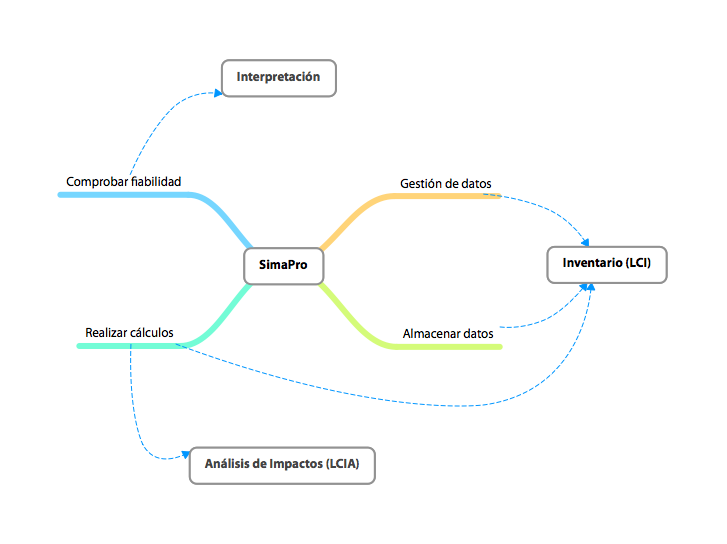
\includegraphics[width=13cm]{img/simapro.png}
\caption{Estructura de SimaPro.}
\label{fig:simapro}
\end{figure}

Entre sus principales cualidades destacan:

\begin{itemize}
  \item Diseño de productos.
  \item Desarrollo de indicadores clave.
  \item Cálculo de la huella de carbono de muchos tipos de productos y sistemas.
  \item Determinar el impacto medioambiental de productos o servicios con precisión estadística mediante el método de análisis Monte Carlo.
  \item Incluye Declaraciones Medioambientales de Productos e Informes Medioambientales GRI (Global Reporting Initiative).
  \item Utilización de bases de datos con inventarios.
  \item Asignación de múltiples procesos de salida.
  \item Análisis de Punto Débil, que permite identifica los puntos sensibles en el ciclo de vida utilizando un árbol de procesos.
  \item Análisis de tratamientos de residuos y escenarios de reciclado.
\end{itemize}

Esta herramienta cuenta con una interfaz de usuario intuitiva con un explorador de guía a través del Análisis de Ciclo de Vida del producto o servicio siguiendo los principios de las normas UNE-EN-ISO 14040:2006 y 14044:2006. Además incorpora un modelado utilizando un asistente paso a paso.

La mayor ventaja de esta herramienta es la utilización de bases de datos con los inventarios de miles de procesos y métodos más importante de análisis de impacto.

SimaPro incluye varias bases de datos de inventarios con miles de procesos, además de los métodos de análisis de impacto más importantes. De esta forma, no es necesario recolectar datos de procesos individuales y poder centrarse en los asuntos más importantes del estudio.

\begin{figure}[!htb]
\centering
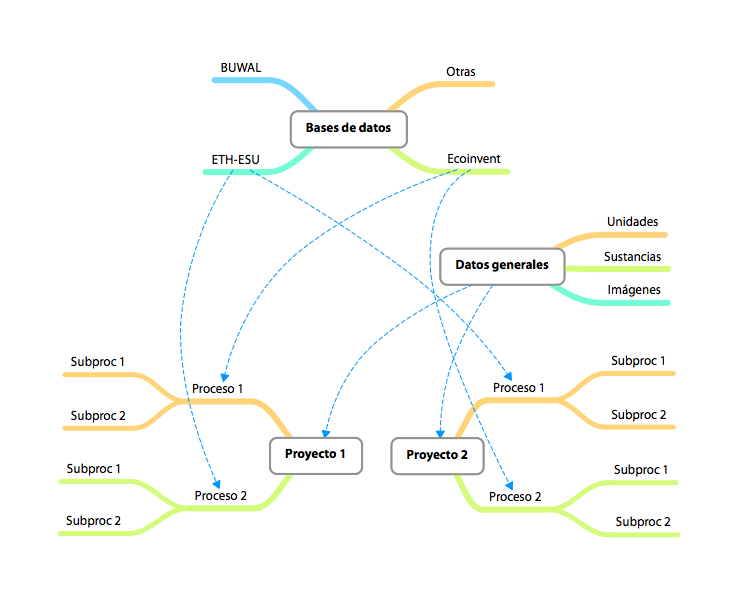
\includegraphics[width=15cm]{img/bbddsimapro.png}
\caption{Estructura de una base de datos de SimaPro.}
\label{fig:bbddsimapro}
\end{figure}

\section{Bases de datos}

La calidad de los datos que aparecen en el Inventario de Ciclo de Vida (ICV) tienen gran importancia en la relevancia del estudio que se realice. En función de la base de datos utilizada el Análisis de Ciclo de Vida puede obtener resultados diferentes.

La metodología de uso del software de Análisis de Ciclo de Vida consiste en utilizar una base de datos como soporte para aquellos materiales y procesos de nuestro sistema que sean similares con los de la base de datos. En caso de que no se adapten a la entrada de la base de datos será necesario modelar una nueva entrada equivalente, pudiendo usar otras entradas de la base de datos.

Cuando se habla de bases de datos (BBDD) en el marco de un ACV, se pueden diferenciar, en función de los datos que contengan, dos tipos:
\begin{itemize}
  \item BBDD con las entradas/salidas que se emplean para simular el sistema analizado en el Inventario de Ciclo de Vida (ICV), conocidas como BBDD de ICV.
  \item BBDD con los datos que cada metodología de Evaluación de Impacto del Ciclo de Vida (EICV) necesita para que la herramienta que llevará a cabo el EICV haga los calculos, conocidas como BBDD de metodologías.
\end{itemize}

Las bases de datos de Inventarios de Ciclo de Vida (ICVs) están formadas por datos de muy diversos materiales y procesos, normalmente agrupados según la fase del ciclo de vida a la que hagan referencia. A través de ellas se puede asignar a cada entrada/salida reflejadas en el ICV una serie de información de la base de datos que indicará la información sobre su impacto ambiental, los factores de caracterización, normalización, etc \cite{ihobecarbono}.

Las bases de datos de metodologías están formadas por los factores de caracterización, ponderación y otros datos que cada metodología de EICV necesita para realizar los cálculos de obtención de resultados. Estas bases de datos recogen los datos en un formato estándar y común (ISO/TS 14048:2002), para que el software de Análisis de Ciclo de Vida pueden utilizar estos datos \cite{ihobecarbono}.

SimaPro (ver sección \ref{sec:simapro}) incorpora varias bases de datos de Inventarios de Ciclo de Vida:
\begin{itemize}
  \item ecoinvent (2009): más de 4000 procesos en energía, transporte, materiales; incluye construcción, químicos, agricultura, etc.; unidad y procesos de sistema.
  \item BUWAL 250 (1997): materiales generales, energía, transporte y desechos, parcialmente basada en base de datos ETH.
  \item ETH-ESU (1996): reconocida base de datos de energía y transporte.
  \item USA Input Output (2003): datos Entrada/Salida para los EE.UU.
  \item Industry data (2001): datos publicados por asociaciones industriales, como APME.
  \item Idemat (2001): base de datos holandesa, recopilada de diferentes fuentes.
  \item Franklin (1996): base de datos generales de EE.UU. sobre materiales, transporte y energía.
  \item Danish IO y Danish Food (2003): bases de datos de Dinamarca de Entrada/Salida y comida.
\end{itemize}

Entre las bases de datos de metodologías de Evaluación de Impactos de Ciclo de Vida, SimaPro incorpora las siguientes:
\begin{itemize}
  \item Efecto 2002: estimación de daños; muchas similitudes con Eco-indicador 99, pero con factores de toxicidad recalculados.
  \item TRACI 2002: método Midpoint desarrollado por US EPA.
  \item CML 2 baseline 2000: actualización del método de 1992, modelos re- avanzados e inclusión de análisis de destino.
  \item EPS 2000: Estimación de daños, usando monetarización (intención de pagar) en lugar de peso por un panel. No hay necesidad de normalización en esta estimación.
  \item Eco-indicator 99: estimación de daños; usa indicadores de categoría en el nivel final. Se incluyen tres versiones usando diferentes suposiciones en los modelos medioambientales.
  \item Ecopoints 97 (UBP): distancia al objetivo basado en objetivos de políticas suizas (conocido también como método de escasez o UBP).
  \item EDIP 97: método de caracterización y normalización desarrollado por EPA de Dinamarca.
  \item Eco-indicator 95: distancia al método objeto basado en objetivos científicos e incluye estimación de daños.
  \item CML 92: método “midpoint” (punto intermedio) bastante usado, caracterización relativamente simple, sin destino o exposición, varios sets de normalización.
\end{itemize}

\subsection{ecoinvent}\label{sec:ecoinvent}

\textit{ecoinvent} implementa en una única base de datos miles de conjuntos de datos de ICVs —agricultura, energía, transporte, combustibles, biomateriales, químicos, materiales de construcción, materiales de empaquetamiento, metales elementales y preciosos, procesado de metales, informática y electrónica, tratamiento de residuos— basados en información industrial recopilada por grupos de investigación y consultores reconocidos internacionalmente \cite{website:ecoinvent}.

\begin{figure}[!htb]
\centering
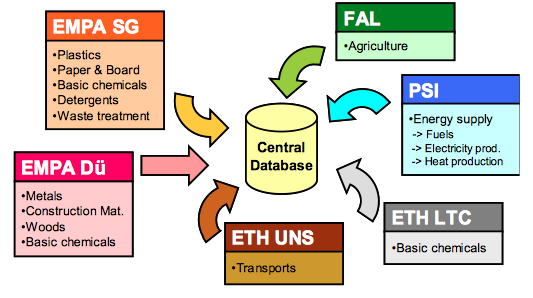
\includegraphics[width=13cm]{img/bbddecoinvent.png}
\caption[Estructura de la base de datos de \textit{ecoinvent}.]{Estructura de la base de datos de \textit{ecoinvent}. Fuente: \protect\cite{mgoedkoop2}.}
\label{fig:bbddecoinvent}
\end{figure}

La base de datos \textit{ecoinvent}:
\begin{itemize}
  \item Incorpora más de 4000 procesos:
  \begin{itemize}
    \item Bienes de producción y calidades.
    \item Para algunos procesos añade diferencias regionales (Suiza y Unión Europea).
    \item Mix eléctrico y procesos agrícolas de Estados Unidos y Asia.
  \end{itemize}
  \item Incertidumbre en los datos.
  \item Ilustraciones de la mayoría de los procesos.
  \item Documentación extensa y consistente de los procesos.
  \item Actualizaciones frecuentes y periódicas.
  \item Incluye versiones de los procesos como Unidad (Proceso 1/U) —más detallado— o como Sistema (Proceso 1/S) —sin información de incertidumbre—.
\end{itemize}

\section{Metodología para Evaluación del Impacto del Ciclo de Vida (EICV)}\label{sec:metodologiaeicv}

La base de datos \textit{ecoinvent} ofrece múltiples métodos para la evaluación de impactos que aplican diferentes factores —caracterización, normalización, peso y daño— a cada flujo elemental de la tabla de inventario según su implementación. Los métodos más destacables que se tendrán en cuenta en este proyecto son:

\begin{itemize}
  \item Método ReCiPe: categorías de impacto y áreas de protección del medio ambiente.
  \item Método de Demanda de Energía Acumulada: cuantificación de energía consumida.
  \item Método IPCC 2007: cálculo potencial del calentamiento global a lo largo del ciclo de vida.
\end{itemize}

\subsection{ReCiPe}\label{sec:recipe}

El desarrollo de ReCiPe se debió al principio a integrar la metodología orientada al problema de \textit{CML-IA} y la metodología orientada al daño de \textit{Ecoindicator 99}. De esta manera, ReCiPe se convirtió en el sucesor de ambos métodos \cite{mgoedkoop3}.

La metodología orientada al problema de \textit{CML-IA} define las categorías de impacto en el punto medio. La incertidumbre de los resultado en este punto es relativamente baja. El inconveniente de este sistema es la ambigüedad de las conclusiones al haber demasiadas categorías de impacto.

La metogología orientada al daño de \textit{Ecoindicator 99} aborda sólo tres categorías de impacto, lo que hacer más fácil obtener conclusiones. Sin embargo, la incertidumbre de los resultados es más alta que con la otra metodología.

ReCiPe implemente ambas estrategias incluyendo las categorías de impacto tanto a punto medio como a punto final. A los factores de caracterización a punto medio se les aplica un factor de daño para obtener los valores de caracterización de punto final. ReCiPe comprende un total de 21 categorías de impacto agrupadas en 2 conjuntos (ver figura ref{recipecategoriasimpacto}):
\begin{itemize}
\item Punto medio: 18 categorías de impacto.
\item Punto final: 3 categorías de impacto.
\end{itemize}

\begin{figure}[!htb]
\centering
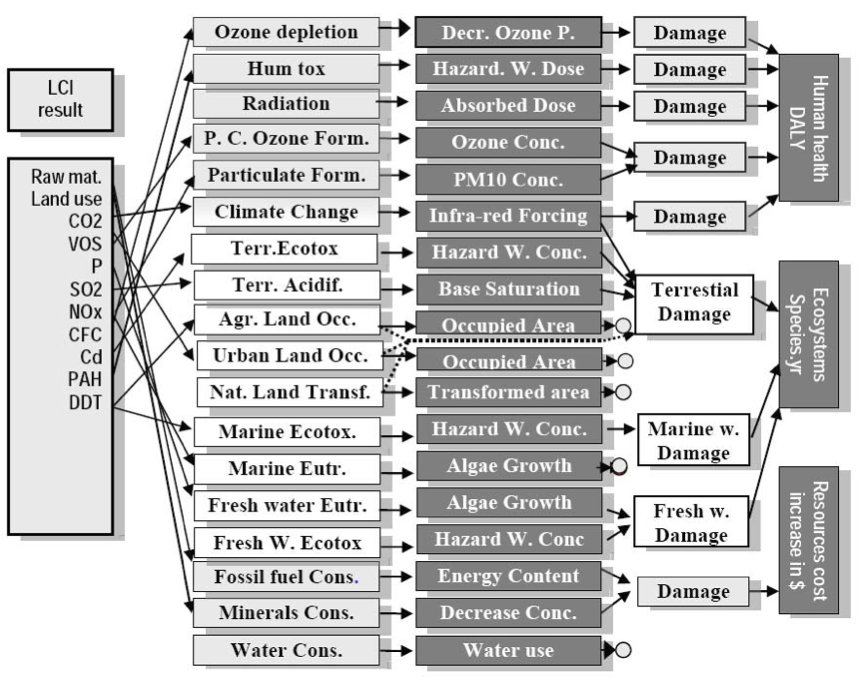
\includegraphics[width=12cm]{img/recipecategoriasimpacto.png}
\caption[Categorías de impacto aplicadas por ReCiPe.]{Categorías de impacto aplicadas por ReCiPe. Fuente: \protect\cite{mgoedkoop3}.}
\label{fig:recipecategoriasimpacto}
\end{figure}

\subsection{Demanda de Energía Acumulada}

Esta metodología —desarrollada a principio de los 70 debido a la crisis del petróleo— permite investigar el uso de energía a través del ciclo de vida de un producto o servicio. El análisis de la Demanda Acumulada de Energía consiste en la cuantificación tanto del uso directo como directo de energía —o consumo gris— durante todo el ciclo de vida del producto \cite{ecoinventlcia}.

Los valores CED (Cumulate Energy Demand) pueden utilizarse para comparar los resultado de un estudio detallada de Análisis de Ciclo de Vida con otros donde se indica únicamente la demanda de energía. También pueden utilizarse como indicador de verificación de los datos ya que es bastante fácil juzgar en base a la Demanda de Energía Acumulada si se han cometido errores importantes o no \cite{ecoinventlcia}.

Debido a que existe divergencias en los conceptos para la caracterización de las fuentes de energía primarias, los indicadores CED se dividen en ocho subcategorías para su uso con la base \textit{ecoinvent}, divididos en dos categorías base:

\begin{itemize}
  \item Fuentes no renovables: fósil, nuclear y bosque primario.
  \item Fuentes renovables: biomasa, viento, solar, geotérmica y agua.
\end{itemize}

\subsection{IPCC 2007}

El método IPCC 2007 —Intergovernmental Panel on Climate Change— es una actualización su homónimo de 2001. Este método es uno de los más empleados en la evaluación de impactos ya que realiza una caracterización de diferentes emisiones gaseosas de acuerdo a su Potencial de Calentamiento Global —Global Warming Potencial, GWP— y al conjunto de diferentes emisiones en la categoría de impacto de calentamiento global. Los valores de caracterización para las emisiones de gases de efecto invernadero se basan en los potenciales de calentamiento global publicados por el propio Grupo Intergubernamental de Expertos sobre el Cambio Climático (IPCC).

Al igual que en la versión de 2001, se establecen tres horizontes temporales para mostrar los efectos de la duración en la atmósfera de los diferentes gases:

\begin{itemize}
  \item GWP 20a (20 años).
  \item GWP 100a (100 años).
  \item GWP 500a (500 años).
\end{itemize}

Los Potenciales de Calentamiento Global (GWPs) directos están relacionados con el impacto del dióxido de carbono (\ce{CO2}). Los GWPs son un índice para la estimación de la contribución de calentamiento global relativo debido a las emisión atmosférica de un kilogramo de un gas de efecto invernadero concreto comparado con la emisión de un kilogramo de \ce{CO2} \cite{ecoinventlcia}.

\section{Categorías de impacto e indicadores de categoría}

En la Evaluación del Inventario del Ciclo de Vida (EICV) se seleccionan categorías de impacto e indicadores de categoría para reflejar los asuntos ambientales relacionados con el sistema del producto bajo estudio. Los modelos de caracterización vinculan los resultados de los inventarios con los indicadores de categoría a través de factores de caracterización. El indicador de categoría es la representación cuantificable de una categoría de impacto de EICV \cite{niembro}.

El indicador de categoría es la causa mesurable en una vía de impacto. El cálculo de las magnitudes de estos indicadores requiere factores de caracterización en función de modelos de caracterización \cite{mlgceballos}.

Una ``categoría de impacto de punto medio'' expresa la visión de que este punto está localizado en algún lugar en el recorrido de impacto como un punto intermedio entre los resultados del Inventario de Ciclo de Vida (ICV) y el daño o punto final del recorrido. En consecuencia, un paso más podría asignar estas categorías de punto medio con una o más categorías de daños, que representan cambios en la calidad del medioambiente. Un indicador de daños es la representación cuantificada de este cambio de calidad, que en la práctica es siempre un modelo simplificado de una realidad muy compleja \cite{ecoinventlcia}.

Una ``categoría de impacto de punto final'' corresponde a una zona de protección donde se forman la base de las decisiones políticas y el desarrollo sostenible. Los áreas de protección fundamentalmente son: salud humana, calidad del ecosistema, disponibilidad de recursos \cite{mlgceballos}.

El método ReCiPe relaciona los datos del ICV con un número determinado de puntos medios, que a su vez se relacionarán con otro número determinado de puntos finales. El método alinea los métodos para la Evaluación de Impacto del Ciclo de Vida con orientación al punto medio con los de orientación al punto final, concretamente el método CML 2002 y el método Ecoindicator 99 \cite{unijaume}. Las relaciones alcanzadas con el método ReCiPe, así como las conexiones entre los puntos medios y los puntos finales en términos de las categorías son:

\begin{itemize}
  \item Cambio climático: CC.
  \item Reducción de la capa de ozono: OD.
  \item Acidificación del medio terrestre: TA.
  \item Eutrofización del agua dulce: FE.
  \item Eutrofización del medio marino: ME.
  \item Toxicidad humana: HT.
  \item Formación de oxidantes fotoquímicos: POF.
  \item Formación de partículas: PMF.
  \item Ecotoxicidad terrestre: TET.
  \item Ecotoxicidad del agua dulce: FET.
\end{itemize}

Por otro lado, existen tres escenarios en el método ReCiPe (al igual que en Ecoindicator 99):

\begin{itemize}
  \item Individualista (I, Individualist): se basa en el corto plazo, las tipologias de impacto no son discutibles y el optimismo tecnológico en cuanto a la adaptación humana. Es la perspectiva más optimista.
  \item Jerárquica (H, Hierarchist): se basa en los principios políticos más comunes en cuanto a plazo temporal y otros problemas.
  \item Igualitaria (E, Egalitarian): es la más catastrofista, pues considera, entre otros, el largo plazo y los impactos que todavía no están plenamente identificados pero para los que existe alguna evidencia.
\end{itemize}

En este proyecto se utilizará únicamente el método de análisis ReCiPe Endpoint (H) V1.06 / Europe ReCipe H/A, como método recomendado por los desarrolladores de SimaPro. En la perspectiva jerárquica (H) se asume que los daños son evitables si se realiza una buena gestión y al uso de la ponderación media (A).

%!TEX root = informe.tex
\chapter{Análisis de Ciclo de Vida de un adoquín: definición del objetivo y alcance}
\section{Objetivo}
Como se indicó en el capítulo \ref{cap:objeto}, el objetivo principal de este proyecto es el Análisis de Ciclo de Vida del adoquín común prefabricado del cemento utilizado en obras civiles y urbanismo, analizando el ciclo de vida del adoquín desde la obtención de la materia prima hasta su fin de vida, es decir, ``desde la cuna hasta la tumba''. El adoquín a estudio es el modelo Holanda 6, de dimensiones 200x100x60 \si{mm}.

La razón principal de este Análisis de Ciclo de Vida es evaluar el comportamiento ambiental de las distintas etapas de su ciclo de vida, las cargas ambientales asociadas a estas etapas e identificar las posibles mejoras.

El público al que se prevé comunicar los resultados de este estudio es principalmente al Tribunal Calificador de Proyectos y a los fabricantes de productos prefabricados del cemento.

No está previsto utilizar los resultados en aseveraciones comparativas con otros materiales y que puedan divulgarse al público.

\section{Alcance}
\subsection{Sistema y sus límites}
Según la norma UNE-EN-ISO 14044:2006 \cite{iso14044}, el \textbf{sistema del producto} ``representa el conjunto de procesos unitarios con sus flujos elementales y flujos de producto'' (representados en la figura XXXX).

% \begin{figure}[!htb]
% \centering
% 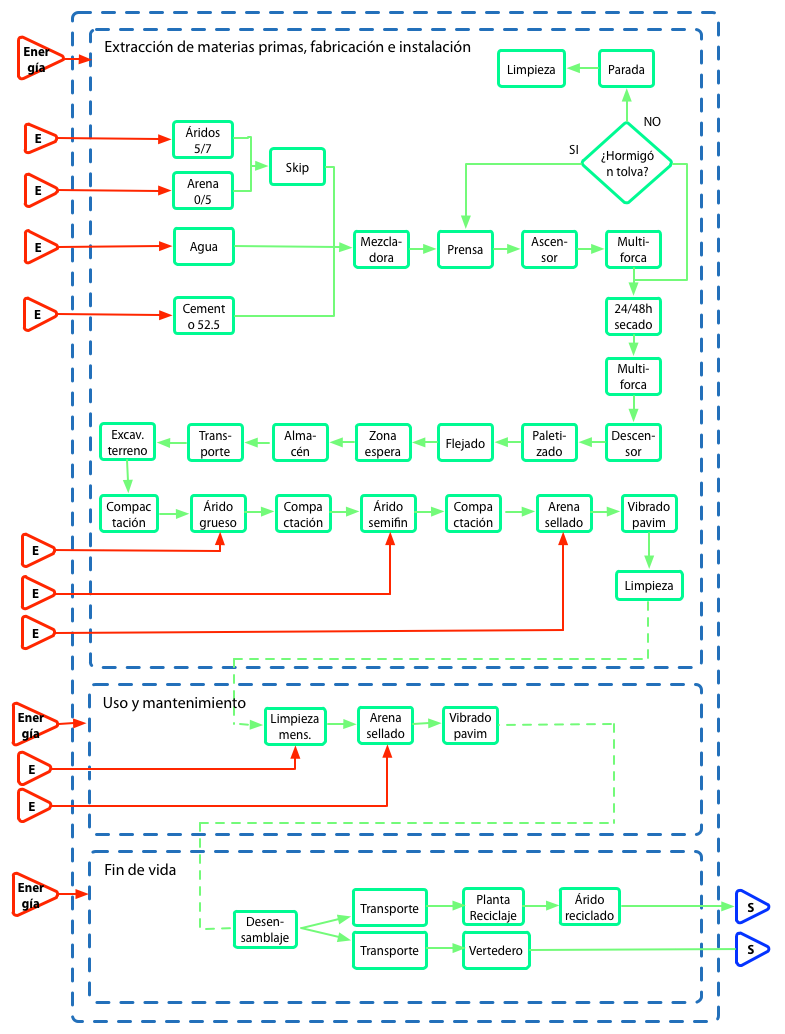
\includegraphics[width=12cm]{sistema.png}
% \caption[Sistema del producto adoquín.]{Sistema del producto adoquín. Fuente: elaboración propia.}
% \label{fig:sistema}
% \end{figure}

También se define \textbf{proceso unitario} como ``el elemento más pequeño considerado en el análisis del inventario del ciclo de vida para el cual se cuantifican lo datos de entrada y salida'', siendo la \textbf{entrada} el ``flujo de producto, de materia o de energía que entra en un proceso unitario'' y la \textbf{salida} el ``flujo de producto, materia o de energía que sale de un proceso unitario''. Por último, el \textbf{flujo de producto} es ``productos que entran o salen de un sistema del producto hacia otro''. Sirvan de ejemplos de proceso unitario en este caso el mezclado del hormigón o la vibrocompresión.

Para el estudio se ha empleado el modelo con mayor demanda de producción de la empresa Malaka de Prefabricados, S.L. y se han utilizado datos proporcionados de la misma (Anexo \ref{apend:datos}) para desarrollar el inventario y los cálculos. El adoquín a estudio es el modelo Holanda 6, de dimensiones 200x100x60 \si{mm} (datos técnicos en Anexo \ref{apend:catalogo}).

% INCLUIR ESTO
% \begin{figure}[!htb]
% \centering
% 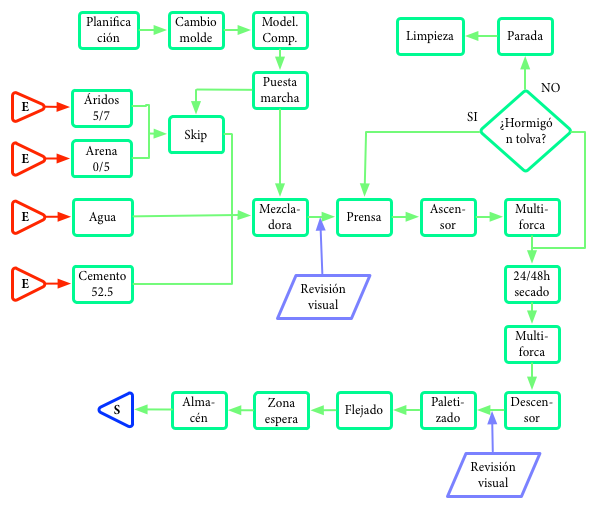
\includegraphics[width=15cm]{diagrama.png}
% \caption{Diagrama de flujo de la fabricación de adoquines.}
% \label{fig:diagrama_de_flujo}
% \end{figure}

\subsection{Unidad funcional}\label{sec:unidad_funcional}
El motivo de tomar como \textit{Unidad funcional} ``1 \si{m^2} de adoquín'' es debido a que los pedidos y la fabricación se realizan en unidades de superficie y no en cantidad de bloques de adoquín. Cada bandeja fabricada supone exactamente 0.5 \si{m^2} de adoquines modelo ``Holanda 6''. Si se toma como \textit{Unidad funcional} 1 \si{m^2} de adoquín, los cálculos se realizan de forma sencilla para 2 bandejas.

\subsection{Límites del sistema}
Los \textbf{límites del sistema} ``definen los procesos unitarios a ser incluido en el sistema'', es decir``determinan qué procesos unitarios se deben incluir dentro del ACV. La selección de los límites del sistema y la exclusión de etapas deben ser coherentes con los objetivos del estudio'' \cite{iso14040}:

\begin{itemize}
  \item No se ha excluido ninguna etapa en el análisis, aunque sea poco significativa.
  \item Los límites del sistema los establece el sistema del producto representado en la figura XXXX. Las entradas/salidas no incluidas se consideran fuera del análisis.
  \item La cantidad total de adoquines son reciclables, aunque se indica que un 5\% se pierde en vertederos llegados allí mezclados con otros residuos \cite{euroadoquin}.
  \item Las capas componentes también pueden ser recicladas, pero sólo se tendrán en cuenta para la instalación y uso de los adoquines, ya que pueden reutilizarse para nuevas instalaciones tras un recambio de la capa de adoquines.
  \item Este proyecto se ha pensado para el área geográfica de Málaga en el año 2013 y tiene datos adaptados para tal caso. Es tal el caso del mix eléctrico, actualizado a fecha de 2013 para España \cite{mlgceballos}.
\end{itemize}

\subsection{Procedimientos de asignación}
Los procedimientos de asignación para futuras aseveraciones comparativas, en el caso que las haya, deberán incluir todas las entradas y salidas que se producen en cada proceso así como las consideradas en este proyecto. Se deberá evitar omitir etapas, procesos, entradas/salidas incluso en el caso de que no altere de forma sustancial los resultados finales.

\subsection{Categorías de impacto seleccionadas}

YYYYYY

\subsection{Suposiciones}
La norma UNE-EN-ISO 14044:2006 \cite{iso14044} indica que ``se deben definir con claridad los criterios de corte para la inclusión inicial de entradas y salidas y las suposiciones sobre las cuales se establecen los criterios de corte'', las cuales son:

\begin{itemize}
  \item La distancia de recorrido desde la fuente de materias primas de áridos, arena y cemento es de 8 \si{km} (Alhaurín de la Torre) para las dos primeras y 30 \si{km} (Málaga-El Palo) para el cemento, ya que no siempre la materia prima procede del mismo sitio.
  \item Los cálculos de transporte se han realizado únicamente de ida para un camión de 16—32 \si{\tonne} que cumple una normativa europea de emisiones EURO 4.
  \item El uso del pavimento de adoquines al que se ha destinado es el \textbf{arterias principales}, que pertenece a la \textbf{categoría de tráfico C1} y una \textbf{calidad de explanada E2} con base granular.
  \item El sellado del pavimento de adoquines se hará únicamente con arena, evitando selladores cementados, para preservar la ventaja de fácil retirada para labores de mantenimiento o trabajo bajo explanada.
  \item El periodo de tiempo entre mantenimiento del sellado del pavimento será de 5 años, cumpliendo con las normas recomendadas \cite{euroadoquinc}.
  \item La distancia de recorrido desde el lugar de desensamblaje del adoquín hasta el vertedero o la planta de reciclado se ha supuesto de 50 \si{km} suponiendo una instalación en el área metropolitana de Málaga.

\end{itemize}

\subsection{Requisitos iniciales de calidad de los datos}
Como requisito de calidad de los datos se debe indicar que los datos han sido recopilados durante el año 2013, por lo que se deben considerar variaciones en los cálculos si se desea extrapolar a otros años. El área geográfica donde se han recopilado los datos es la provincia de Málaga (España).

Los datos de partida que se han utilizado en este análisis han sido proporcionados por Malaka de Prefabricados (Apéndice \ref{apend:datos}). La figura \ref{fig:diagrama_de_flujo} muestra las entradas al sistema, así como los procesos que ocurren durante la fabricación —que serán explicados en las siguientes secciones— y la salida del sistema.

%!TEX root = informe.tex
\chapter{Análisis de Ciclo de Vida de un adoquín: Inventario del Ciclo de Vida}\label{cap:acv_inventario}

\section{Introducción}\label{sec:intro_icv}
Como se ha mencionado en la sección \ref{sec:etapaslca}, el Inventario del Ciclo de Vida (ICV) implica la recopilación de los datos y los procedimientos de cálculo para cuantificar las entradas y salidas pertinentes del sistema del producto. Es un proceso iterativo, ya que a medida que se recopilan datos, se aprende más sobre el sistema y se pueden identificar nuevos requisitos o limitaciones que requieran cambios en los procedimientos de recopilación de datos \cite{iso14040}. Los datos pueden clasificarse como:

\begin{itemize}
  \item las entradas de energía, materias primas, entradas auxiliares y otras entradas físicas;
  \item los productos, coproductos y residuos;
  \item las emisiones al aire, los vertidos al agua y suelo;
  \item otros aspectos ambientales.
\end{itemize}

Los datos para cada unidad de proceso del sistema del producto se obtienen bien de la industria o bien de bases de datos. En este caso se ha utilizado la base de datos \textit{ecoinvent} v2.2 (explicada en la sección \ref{sec:ecoinvent}).

Existen cinco etapas principales, de las cuales las tres primeras se agrupan en la etapa de fabricación:
\begin{itemize}
  \item Adquisición de materias primas: actividades necesarias para la extracción de las materias primas y aportaciones de energía del medio ambiente, incluyendo el transporte previo a la producción.
  \item Procesado de materias primas: actividades necesarias para convertir las materias primas en una forma que pueda ser utilizada para fabricar un producto.
  \item Fabricación y montaje: actividades necesarias para convertir los materiales en el producto deseado listado para ser transportado y distribuido.
  \item Uso y mantenimiento: utilización del producto acabado a lo largo de su vida en servicio, incluyendo materias primas y energía.
  \item Fin de vida: una vez que el producto ha servido para su función inicial y consecuentemente se recicla a través del mismo sistema de producto (ciclo cerrado de reciclaje) o entra en un nuevo sistema de producto (ciclo de reciclaje abierto), incluyendo energía y desechos.
\end{itemize}

\section{Fase de extracción de materias primas, fabricación e instalación}

\subsection{Bases del modelado para la extracción de materias primas y fabricación}\label{sec:basesfabricacion}
Cada adoquín mide 200x100x60 \si{mm} y tiene una masa de 3 \si{kg}. Cada bandeja está formada por 25 adoquines, por lo que son necesarias 2 bandejas para tener la \textit{Unidad funcional} de 1 \si{m^2}, con un total de 50 adoquines/\si{m^2} (ecuación \ref{eq:masa}):

\begin{gather}
200 mm \times 100 mm \times 25\ ud/bandeja \times 2\ bandejas = 1 m^2\\
3 kg/ud \times 50 ud/m^2 = 150 kg/m^2 \text{ de masa para adoquín}\label{eq:masa}
\end{gather}

Para disponer de 150 \si{kg/m^2} de masa para adoquín se aplican los porcentajes de materias primas sobre la fórmula base para adoquín ``Holanda 6'' proporcionada por el fabricante para obtener las masas de cada materia prima reflejadas en la tabla \ref{desglosemateriasprimas}.

\begin{table}[!htb]
\centering
\begin{tabular}{lcccc}
\toprule
\multicolumn{5}{c}{Consumo de materias primas por \si{m^2} de adoquín fabricado}\\
\midrule
Materia prima & \% Fórmula & Masa (\si{kg}) & Proced. & Dist. (\si{km})\\
\midrule
Árido tipo 5/7 & 37.75 & 56.63 & Alh. Torre & 8\\
Arena tipo 0/5 & 47.16 & 70.74 & Alh. Torre & 8\\
Cemento Portland 52.5N & 10.06 & 15.09 & Málaga-El Palo & 30\\
Agua & 5.03 & 7.54 & Red & -\\
\bottomrule
\end{tabular}
\caption{Desglose de materias primas por \si{m^2} de adoquín fabricado.}
\label{desglosemateriasprimas}
\end{table}

En el Anexo \ref{apend:catalogo} también se especifica un diagrama de Gantt de los procesos para una simulación realizada para fabricar 1 \si{m^2} de adoquín, además de los consumos energéticos desglosados.

A la hora de realizar el inventario de esta fase es necesario tener en cuenta la vida útil de las instalaciones donde se realiza el proceso de fabricación. El fabricante estima esta vida útil en 15 años con una fabricación media anual de 12000 \si{m^2}. Por tanto, los modelados se dividirán entre un factor de proporcionalidad FF de 180000 (ver ecuación \ref{ec:ff}).

\begin{equation}\label{ec:ff}
FF = 12000\ m^2/a \times 15\ a = 180000 m^2 \text{ en 15 años}\\
\end{equation}

\subsection{Cemento}
El cemento se transporta a granel en camiones con tanques a presión hasta la fábrica. Allí se almacena en silos provistos de compresores que descargan el material desde el tanque hasta su interior. El compresor es alimentado por electricidad mediante una toma de corriente conectada a la red eléctrica. La descarga del silo es únicamente por gravedad con válvulas dosificadoras de control de caudal (ver tabla \ref{modeladodelcemento}).

Las unidades para el modelado del camión (lorry) vienen expresadas en \si{kg\times km}, mientras que el uso del silo se proporciona en \si{m^3}, dada una densidad media del cemento Portland de 1250 \si{kg/m3} \cite{website:cement}.

\begin{gather}
15.09 kg \times 30 km = 453 kg\times km\\
15,09 kg / 1250 kg/m^3 = 0.0121 m^3
\end{gather}

El mix eléctrico se obtiene del consumo del compresor del silo proporcional a una cantidad de 15.09 \si{kg}, si la potencia del compresor son 30kW, velocidad de carga del silo es 35 \si{\tonne/h} para un tiempo de llenado de 35 minutos.

\begin{gather}
30 kW \times 1 h \times \frac{35 min}{60 min} = 17.5 kWh = 63 MJ \text{ para 20 toneladas}\\
35 t/h \times \frac{35 min}{60 min} = 20 t \text{ de cemento con el silo cargado}\\
15.09 kg \times \frac{63 MJ}{20 t} = 4.79 kJ
\end{gather}

\begin{table}[!htb]
\centering
\begin{tabular}{p{8cm}rc}
\toprule
\multicolumn{3}{c}{Cemento Portland CEM I 52.5Z gris}\\
\midrule
Materiales/ensamblajes & Cantidad & Unidad\\
\midrule
Portland cement, strength class Z 52.5, at plant/CH U & 15.09 & \si{kg}\\
\midrule
Procesos & Cantidad & Unidad\\
\midrule
Transport, lorry 16-32t, EURO4/RER U & 453 & \si{kg*km}\\
Tower silo, plastic/CH/I U & 0.0121 & \si{m^3}\\
Electricity mix 2013/ES U & 4.79 & \si{kJ}\\
\bottomrule
\end{tabular}
\caption{Modelado del cemento.}
\label{modeladodelcemento}
\end{table}

\subsection{Arena y áridos}
Las arenas y áridos se transportan hasta la planta de fabricación mediante camiones. Actualmente los áridos y la arena ya no se apilan a bajo techados en las explanadas adyacentes a las plantas, sino que el propio transporte rellena las tolvas de forma automática.

El tipo de arena que se utiliza en la planta es 0/5 —granulometría en milímetros de las partículas que forman la arena— no está directamente disponible en SimaPro. En su lugar, se ha optado por tomar el material ``Sand 0/2'' (Arena tipo 0/2), que además de pertenecer a la clasificación general de arena —de 0 a 5 \si{mm}—, la descripción de SimaPro indica que puede utilizarse como árido natural estándar en la industria de la construcción (ver tabla \ref{modeladodelaarena}).

\begin{quote}
Technical purpose of product or process: Standard mineral product used as natural aggregates in the construction industry according to the applied technology.
\end{quote}

Las unidades para el modelado del camión (lorry) vienen expresadas en \si{kg\times km}.

\begin{equation}
70.74 kg \times 8 km = 566 kg\times km
\end{equation}

\begin{table}[!htb]
\centering
\begin{tabular}{p{8cm}rc}
\toprule
\multicolumn{3}{c}{Arena tipo 0/5}\\
\midrule
Materiales/ensamblajes & Cantidad & Unidad\\
\midrule
Sand 0/2, wet and dry quarry, production mix, at plant, undried/RER S & 70.74 & \si{kg}\\
\midrule
Procesos & Cantidad & Unidad\\
\midrule
Transport, lorry 16-32t, EURO4/RER U & 566 & \si{kg*km}\\
\bottomrule
\end{tabular}
\caption{Modelado de la arena.}
\label{modeladodelaarena}
\end{table}

Los áridos utilizados para producir adoquines puede incluir arena, gravilla y piedra de machaqueo si se pretende obtener un producto de peso normal. Si se desea que el adoquín sea más ligero —entre un 20 y un 45 \%— sin mermar sus propiedades estructurales se utilizan materiales como pizarra, arcilla, escoria de altos hornos y cenizas de carbón según su disponibilidad y coste.

El tipo de árido utilizado en planta es de granulometría 5/7 —en milímetros—, catalogado como gravilla. No está directamente disponible en SimaPro, por lo que en su lugar, se ha optado por tomar el material ``Gravel, crushed'' (gravilla de machaqueo) (tabla \ref{modeladodearido}).

Las unidades para el modelado del camión (lorry) vienen expresadas en \si{kg\times km}.

\begin{equation}
56.63 kg \times 8 km = 566 kg\times km
\end{equation}

\begin{table}[!htb]
\centering
\begin{tabular}{p{8cm}rc}
\toprule
\multicolumn{3}{c}{Árido tipo 5/7}\\
\midrule
Materiales/ensamblajes & Cantidad & Unidad\\
\midrule
Gravel, crushed, at mine/CH U & 56.63 & \si{kg}\\
\midrule
Procesos & Cantidad & Unidad\\
\midrule
Transport, lorry 16-32t, EURO4/RER U & 453 & \si{kg*km}\\
\bottomrule
\end{tabular}
\caption{Modelado del árido.}
\label{modeladodearido}
\end{table}

\subsection{Agua}
La mayoría de las plantas tienen una fuente de agua municipal (\textit{tap water}) que proporciona potable perfectamente válida para el uso en la fabricación de hormigón (ver tabla \ref{modeladodelagua}).

\begin{table}[!htb]
\centering
\begin{tabular}{p{8cm}rc}
\toprule
\multicolumn{3}{c}{Agua}\\
\midrule
Materiales/ensamblajes & Cantidad & Unidad\\
\midrule
Tap water, at user/RER U & 7.54 & \si{kg}\\
\bottomrule
\end{tabular}
\caption{Modelado del agua.}
\label{modeladodelagua}
\end{table}

\subsection{Mix eléctrico}

El mix eléctrico es la cesta energética de un país, es decir, la combinación de las diferentes fuentes de energía que cubren su suministro eléctrico. Es un indicador de las fuentes energéticas que se emplean para producir electricidad. Cuanto más bajo es el mix, mayor es la contribución de fuentes energéticas bajas en carbono.

Disponer de un mix eléctrico actualizado ayuda a obtener unos resultados más precisos en el Análisis de Ciclo de Vida. La base de datos de \textit{ecoinvent} proporciona un modelo no actualizado para España, sobretodo teniendo en cuenta los últimos avances en adopción de energías renovables en el sector energético español. De esta forma, se ha añadido un nuevo modelo (tabla \ref{modeladomixelectrico}) con las cifras actualizadas al presente año para 1 \si{kWh} \cite{mlgceballos}.

\begin{table}[!htb]
\centering
\begin{tabular}{p{8cm}rc}
\toprule
\multicolumn{3}{c}{Electricity mix 2013/ES U}\\
\midrule
Materiales/combustibles & Cantidad & Unidad\\
\midrule
Electricity, hard coal, at power plant/ES U & 0.0596 & \si{kWh}\\
Electricity, lignite, at power plant/ES U & 0.0268 & \si{kWh}\\
Electricity, oil, at power plant/ES U & 0.0527 & \si{kWh}\\
Electricity, natural gas, at power plant/ES U & 0.3025 & \si{kWh}\\
Electricity, industrial gas, at power plant/ES U & 0.0147 & \si{kWh}\\
Electricity, hydropower, at power plant/ES U & 0.131 & \si{kWh}\\
Electricity, hydropower, at pumped storage power plant/ES U & 0.020 & \si{kWh}\\
Electricity, nuclear, at power plant/UCTE U & 0.205 & \si{kWh}\\
Electricity, production mix photovoltaic, at plant/ES U & 0.024 & \si{kWh}\\
Electricity, at wind power plant/RER U & 0.1454 & \si{kWh}\\
Electricity, at cogen with biogas engine, allocation exergy/CH U & 0.0146 & \si{kWh}\\
Electricity, production mix FR/FR U & 0.0056 & \si{kWh}\\
\bottomrule
\end{tabular}
\caption[Modelado del mix eléctrico español en 2013.]{Modelado del mix eléctrico español en 2013. Fuente: \cite{mlgceballos}.}
\label{modeladomixelectrico}
\end{table}

\subsection{Dosificador de arena y áridos}

El sistema de control central manda una señal a los dosificadores para que viertan la cantidad ordenada por el programa principal de fabricación. Dichos dosificadores consisten en una especie de tolva con forma de embudo con un cierre controlado por el sistema.

No existe un modelo de referencia en SimaPro para este tipo de dosificadores —\textit{feed hopper}, en inglés—, por lo que se ha simplificado un modelo válido \cite{woodpellet}. Se le ha añadido la parte de mix eléctrico de los datos del fabricante (Apéndice \ref{apend:datos}). El dosificador del cemento y del agua están incluidos en su propio modelo (silo y abastecimiento de la red respectivamente).

\begin{table}[!htb]
\centering
\begin{tabular}{p{8cm}rc}
\toprule
\multicolumn{3}{c}{Dosificadores para arena y áridos}\\
\midrule
Materiales/combustibles & Cantidad & Unidad\\
\midrule
Steel, low-alloyed, at plant/RER U & 47 & \si{kg}\\
\midrule
Electricidad/calor & Cantidad & Unidad\\
\midrule
Electricity mix 2013/ES U & 0.0021 & \si{MJ}\\
\bottomrule
\end{tabular}
\caption{Modelado de los dosificadores para arena y áridos.}
\label{modeladodedosificadores}
\end{table}

\subsection{Cintas transportadoras de áridos y cemento}

Las tolvas descargan la cantidad programada de materia prima sobre dos cintas transportadoras —una para áridos y arena, otra para cemento— con básculas de pesaje incorporadas que se comunican con el sistema de control y cortan el flujo de descarga.

La cinta de áridos descarga sobre un skip que eleva los materiales hasta una mezcladora. La cinta de cemento descarga directamente sobre la mezcladora.

Las distancias están medidas sobre planos (Apéndice \ref{planos}), y los consumos se han obtenido de los ensayos en fábrica a partir de la potencia de la cinta transportadora y el tiempo de funcionamiento (Potencia=Energía/Tiempo).

\begin{table}[!htb]
\centering
\begin{tabular}{p{8cm}rc}
\toprule
\multicolumn{3}{c}{Cinta transportadora para arena y áridos}\\
\midrule
Materiales/combustibles & Cantidad & Unidad\\
\midrule
Conveyor belt, at plant/RER/I U & 14.6 & \si{m}\\
\midrule
Electricidad/calor & Cantidad & Unidad\\
\midrule
Electricity mix 2013/ES U & 0.1827 & \si{MJ}\\
\bottomrule
\end{tabular}
\caption{Modelado de la cinta transportadora para arena y áridos.}
\label{modeladodecintaarena}
\end{table}

\begin{table}[!htb]
\centering
\begin{tabular}{p{8cm}rc}
\toprule
\multicolumn{3}{c}{Cinta transportadora para cemento}\\
\midrule
Materiales/combustibles & Cantidad & Unidad\\
\midrule
Conveyor belt, at plant/RER/I U & 7.3 & \si{m}\\
\midrule
Electricidad/calor & Cantidad & Unidad\\
\midrule
Electricity mix 2013/ES U & 0.0975 & \si{MJ}\\
\bottomrule
\end{tabular}
\caption{Modelado de la cinta transportadora para cemento.}
\label{modeladodecintacemento}
\end{table}

\subsection{Skip y mezcladora}

Para asegurar la consistencia del lote el agua se añade mediante un sistema electrónico de control que dosifica el caudal. En el caso de que haya otros aditivos, tales como acelerantes o colorantes, es en este momento cuando se incorporan a la mezcla. Cuando se termina de añadir el agua se produce el mezclado creando hormigón fresco.

La base de datos \textit{ecoinvent} proporciona un modelo para el mezclado del hormigón, ``Paster mixing'' en el que se introduce la masa de la mezcla, 150 \si{kg} y al que se le añade la parte de mix eléctrico de los datos del fabricante (Apéndice \ref{apend:datos}).

\begin{table}[!htb]
\centering
\begin{tabular}{p{8cm}rc}
\toprule
\multicolumn{3}{c}{Skip y mezcladora}\\
\midrule
Materiales/combustibles & Cantidad & Unidad\\
\midrule
Plaster mixing/CH U & 150 & \si{kg}\\
\midrule
Electricidad/calor & Cantidad & Unidad\\
\midrule
Electricity mix 2013/ES U & 1.71 & \si{MJ}\\
\bottomrule
\end{tabular}
\caption{Modelado del skip y la mezcladora.}
\label{modeladoskip}
\end{table}

\subsection{Cinta transportadora para hormigón}

El hormigón sale de la mezcladora mediante una cinta transportadora que contiene otra báscula de pesaje y se dirige hacia la tolva de hormigón que se encuentra en lo alto de la prensa.

La base de datos \textit{ecoinvent} proporciona un modelo para la cinta transportadora, ``Conveyor belt'' en el que se introduce la distancia de recorrido, 12.1 \si{m}, y al que se le añade la parte de mix eléctrico de los datos del fabricante (Apéndice \ref{apend:datos}).

\begin{table}[!htb]
\centering
\begin{tabular}{p{8cm}rc}
\toprule
\multicolumn{3}{c}{Cinta transportadora para hormigón}\\
\midrule
Materiales/combustibles & Cantidad & Unidad\\
\midrule
Conveyor belt, at plant/RER/I U & 12.1 & \si{m}\\
\midrule
Electricidad/calor & Cantidad & Unidad\\
\midrule
Electricity mix 2013/ES U & 0.088 & \si{MJ}\\
\bottomrule
\end{tabular}
\caption{Modelado de la cinta transportadora para hormigón.}
\label{modeladodecintahormigon}
\end{table}

\subsection{Tolva para hormigón}

La tolva de hormigón se encarga de dosificar el hormigón en el molde de la prensa. No existe un modelo de referencia en SimaPro para tolvas —\textit{hopper}, en inglés—, por lo que se ha simplificado un modelo válido \cite{foodnottrash}. Se le ha añadido la parte de mix eléctrico de los datos del fabricante (Apéndice \ref{apend:datos}).

\begin{table}[!htb]
\centering
\begin{tabular}{p{8cm}rc}
\toprule
\multicolumn{3}{c}{Tolva para hormigón}\\
\midrule
Materiales/combustibles & Cantidad & Unidad\\
\midrule
Steel, low-alloyed, at plant/RER U & 470 & \si{kg}\\
\midrule
Electricidad/calor & Cantidad & Unidad\\
\midrule
Electricity mix 2013/ES U & 0.0161 & \si{MJ}\\
\bottomrule
\end{tabular}
\caption{Modelado de la tolva para hormigón.}
\label{modeladotolvahormigon}
\end{table}

\subsection{Vibrocompresión}

La tolva dosifica el hormigón fresco, que cae en los moldes para adoquines. Los moldes tienen una longevidad muy alta —aproximadamente un millón de ciclos de prensado— y su durabilidad depende de las propiedades abrasivas de los áridos utilizados.

El molde se compone de dos partes: la parte donde se inyecta el hormigón (hembra) y la parte que se coloca encima para dar forma (macho). La prensa tiene incorporado un carro alimentador encargado de proporcionar la parte hembra. Se inyecta el hormigón en el molde hembra, el molde macho baja con la prensa y el hormigón es compactado y cimentado usando un sistema combinado de presión y vibración. Cada molde puede producir 25 adoquines de 200x100x60\si{\milli\meter}, lo que proporciona a una superficie adoquinada de 0.5\si{\square\meter}. Los adoquines son moldeados de una sola pieza y extraidos del molde inmediatamente después de la vibro-compresión sobre una bandeja de madera.

SimaPro no proporciona un modelo para prensas de cemento. Estudiando las similitudes entre una planta de hormigón —\textit{concrete plant}— y la planta objeto de este proyecto, se puede aproximar un modelo de la prensa basado en la maquinaria del primero \cite{buildingproducts}. La aproximación ``Industrial machine, heavy, unspecified, at plant'' pide la masa de la máquina industrial no específica que realiza el proceso. De acuerdo al fabricante, ese dato es de 1380 \si{kg}, al que se le ha añadido la parte de mix eléctrico también proporcionado por el fabricante (Apéndice \ref{apend:datos}).

\begin{table}[!htb]
\centering
\begin{tabular}{p{8cm}rc}
\toprule
\multicolumn{3}{c}{Prensado}\\
\midrule
Materiales/combustibles & Cantidad & Unidad\\
\midrule
Industrial machine, heavy, unspecified, at plant/RER/I U & 9000 & \si{kg}\\
\midrule
Electricidad/calor & Cantidad & Unidad\\
\midrule
Electricity mix 2013/ES U & 0.437 & \si{MJ}\\
\bottomrule
\end{tabular}
\caption{Modelado del prensado.}
\label{modeladoprensado}
\end{table}

\subsection{Cinta transportadora para piezas frescas}

La bandeja con las piezas frescas es trasladada sobre un transportador de rodillos hasta un ascensor.

SimaPro no proporciona un modelo para este tipo de transportador. Estudiando las similitudes entre un transportador de rodillos y una cinta transportadora se puede aproximar un modelo propio basado en que la principal diferencia es la falta de una banda de rodadura (tabla \ref{modeladotransportadorrodillos}).

\begin{table}[!htb]
\centering
\begin{tabular}{p{8cm}rc}
\toprule
\multicolumn{3}{c}{Transportadora de rodillos para piezas frescas}\\
\midrule
Materiales/combustibles & Cantidad & Unidad\\
\midrule
Concrete, sole plate and foundation, at plant/CH U & 0.01 & \si{m^3}\\
Section bar rolling, steel/RER U & 500 & \si{kg}\\
Steel, low-alloyed, at plant/RER U & 530 & \si{kg}\\
Transport, lorry >16t, fleet average/RER U & 55.5 & \si{\tonne\times km}\\
Wire drawing, steel/RER U & 29.6 & \si{kg}\\
\midrule
Residuos y emisiones para tratamiento & Cantidad & Unidad\\
\midrule
Disposal, building, reinforced concrete, to final disposal/CH U & 23 & \si{kg}\\
Disposal, steel, 0\% water, to municipal incineration/CH U & 29.6 & \si{kg}\\
\bottomrule
\end{tabular}
\caption{Modelado de 1 metro de transportador de rodillos.}
\label{modeladotransportadorrodillos}
\end{table}

La aproximación ``Roller conveyor, at plant'' pide como parámetro la distancia de recorrido, 6.8 \si{m}, al que se le ha añadido la parte de mix eléctrico también proporcionado por el fabricante (Apéndice \ref{apend:datos}).

\begin{table}[!htb]
\centering
\begin{tabular}{p{8cm}rc}
\toprule
\multicolumn{3}{c}{Transportadora de rodillos para piezas frescas}\\
\midrule
Materiales/combustibles & Cantidad & Unidad\\
\midrule
Conveyor belt, at plant/RER/I U & 6.8 & \si{m}\\
\midrule
Electricidad/calor & Cantidad & Unidad\\
\midrule
Electricity mix 2013/ES U & 0.077 & \si{MJ}\\
\bottomrule
\end{tabular}
\caption{Modelado del transportador de rodillos para piezas frescas.}
\label{modeladotransportadorpiezas}
\end{table}

\subsection{Ascensor}

Este ascensor tiene diez alturas, de forma que cada vez que recibe una bandeja con adoquines frescos, la bandeja anterior sube una altura y monta la siguiente. El ascensor se encarga de alimentar un carro multiforca de diez alturas.

SimaPro no proporciona un modelo para un ascensor de estas características, por lo que se ha obtado por un elemento genérico que sí esté en la base de datos de \textit{ecoinvent} como ``Industrial machine, heavy, unspecified, at plant'' que pide la masa de la máquina industrial no específica que realiza el proceso. De acuerdo al fabricante, ese dato es de 320 \si{kg}, al que se le ha añadido la parte de mix eléctrico también proporcionado por el fabricante (Apéndice \ref{apend:datos}).

\begin{table}[!htb]
\centering
\begin{tabular}{p{8cm}rc}
\toprule
\multicolumn{3}{c}{Ascensor}\\
\midrule
Materiales/combustibles & Cantidad & Unidad\\
\midrule
Industrial machine, heavy, unspecified, at plant/RER/I U & 320 & \si{kg}\\
\midrule
Electricidad/calor & Cantidad & Unidad\\
\midrule
Electricity mix 2013/ES U & 0.126 & \si{MJ}\\
\bottomrule
\end{tabular}
\caption{Modelado del ascensor.}
\label{modeladodelascensor}
\end{table}

\subsection{Multiforca}
Cuando las diez alturas está ocupadas se cargan en un carro multiforca —\textit{rack transporter}, en inglés— automatizado que transporta las piezas hasta un secadero.

Las piezas permanecen en el secadero curándose a temperatura ambiente entre 24 y 48 horas.

Una vez transcurrido el tiempo de curado, los adoquines están secos y listos para ser recogidos por otro carro multiforca automatizado que recoge las bandejas y las lleva a un descensor.

SimaPro tampoco proporciona un modelo para un carro multiforca, por lo que también se ha obtado por un elemento genérico que sí esté en la base de datos de \textit{ecoinvent} como ``Industrial machine, heavy, unspecified, at plant'' que pide la masa de la máquina industrial no específica que realiza el proceso. De acuerdo al fabricante, un carro multiforca se compone de un tres partes: transportador de forca (rackveyor), rodadura (crawler) y vehículo (transfer car), sumando en total 7500 \si{kg}, a lo que se le ha añadido la parte de mix eléctrico también proporcionado por el fabricante (Apéndice \ref{apend:datos}).

\begin{table}[!htb]
\centering
\begin{tabular}{p{8cm}rc}
\toprule
\multicolumn{3}{c}{Multiforca}\\
\midrule
Materiales/combustibles & Cantidad & Unidad\\
\midrule
Industrial machine, heavy, unspecified, at plant/RER/I U & 7500 & \si{kg}\\
\midrule
Electricidad/calor & Cantidad & Unidad\\
\midrule
Electricity mix 2013/ES U & 0.516 & \si{MJ}\\
\bottomrule
\end{tabular}
\caption{Modelado de la multiforca.}
\label{modeladomultiforca}
\end{table}

\subsection{Descensor}
El descensor coloca las bandejas con los adoquines secos en un transportador de rodillos. Su modelado es el mismo que el del ascensor.

\begin{table}[!htb]
\centering
\begin{tabular}{p{8cm}rc}
\toprule
\multicolumn{3}{c}{Descensor}\\
\midrule
Materiales/combustibles & Cantidad & Unidad\\
\midrule
Industrial machine, heavy, unspecified, at plant/RER/I U & 320 & \si{kg}\\
\midrule
Electricidad/calor & Cantidad & Unidad\\
\midrule
Electricity mix 2013/ES U & 0.126 & \si{MJ}\\
\bottomrule
\end{tabular}
\caption{Modelado del descensor.}
\label{modeladodeldescensor}
\end{table}

\subsection{Transporte de bandejas hasta paletizadora}
El transportador de rodillos lleva las bandejas hasta una paletizadora para hacer bloques de hasta cinco alturas. Se ha vuelto a utilizar el modelado de la tabla \ref{modeladotransportadorrodillos}, introduciendo los 6.88 \si{m} de recorrido entre el origen y el destino, a lo que se le ha añadido la parte de mix eléctrico también proporcionado por el fabricante (Apéndice \ref{apend:datos}).

\begin{table}[!htb]
\centering
\begin{tabular}{p{8cm}rc}
\toprule
\multicolumn{3}{c}{Transporte de bandejas hasta paletizadora}\\
\midrule
\multicolumn{2}{c}{Materiales/combustibles}\\
\cmidrule(r){1-2}
Descripción & Cantidad & Unidad\\
\midrule
Roller conveyor, at plant/RER/I U & 6.88 & \si{m}\\
\midrule
\multicolumn{2}{c}{Electricidad/calor}\\
\cmidrule(r){1-2}
Descripción & Cantidad & Unidad\\
\midrule
Electricity mix 2013/ES U & 0.021 & \si{MJ}\\
\bottomrule
\end{tabular}
\caption{Modelado del transporte de bandejas hasta paletizadora.}
\label{modeladobandejaspalet}
\end{table}

\subsection{Paletizado y flejado}

La paletizadora dispone los bloques de adoquín sobre un pallet para su posterior almacenaje y transporte. De esta forma se consigue una mayor uniformidad y facilidad de manipulación de la carga, ahorrando espacio y rentabilizando los tiempos de carga—descarga y manipulación.

La paletizadora impulsa el pallet hasta la flejadora que aplica varias lazadas de flejes para evitar que los adoquines se desprendan del conjunto.

El proceso de SimaPro ``Packing, clay products'' abarca ambos procesos en un único modelo, en el que se introduce la masa de la carga, 150 \si{km}, a lo que se le ha añadido la parte de mix eléctrico proporcionado por el fabricante (Apéndice \ref{apend:datos}).

\begin{table}[!htb]
\centering
\begin{tabular}{p{8cm}rc}
\toprule
\multicolumn{3}{c}{Flejado y paletizado}\\
\midrule
Materiales/combustibles & Cantidad & Unidad\\
\midrule
Packing, clay products/CH U & 150 & \si{kg}\\
\midrule
Electricidad/calor & Cantidad & Unidad\\
\midrule
Electricity mix 2013/ES U & 0.065 & \si{MJ}\\
\bottomrule
\end{tabular}
\caption{Modelado del flejado y paletizado.}
\label{modeladodelflejadoypaletizado}
\end{table}

\begin{table}[!htb]
\centering
\begin{tabular}{p{8cm}rc}
\toprule
\multicolumn{3}{c}{Transporte de pallets hasta flejadora}\\
\midrule
Materiales/combustibles & Cantidad & Unidad\\
\midrule
Roller conveyor, at plant/RER/I U & 3.1 & \si{m}\\
\midrule
Electricidad/calor & Cantidad & Unidad\\
\midrule
Electricity mix 2013/ES U & 0.021 & \si{MJ}\\
\bottomrule
\end{tabular}
\caption{Modelado del transporte de pallets hasta flejadora.}
\label{modeladopalletsflejadora}
\end{table}

\subsection{Transporte de pallets flejados hasta zona de recogida}

La flejadora descansa los conjuntos paletizados sobre un un transportador de rodillos para ser posteriormente llevados a almacén.

\begin{table}[!htb]
\centering
\begin{tabular}{p{8cm}rc}
\toprule
\multicolumn{3}{c}{Transporte de pallets flejados hasta zona de recogida}\\
\midrule
Materiales/combustibles & Cantidad & Unidad\\
\midrule
Roller conveyor, at plant/RER/I U & 39.1 & \si{m}\\
\midrule
Electricidad/calor & Cantidad & Unidad\\
\midrule
Electricity mix 2013/ES U & 0.0315 & \si{MJ}\\
\bottomrule
\end{tabular}
\caption{Modelado del transporte de pallets flejados hasta zona de recogida.}
\label{modeladopalletsrecogida}
\end{table}

\subsection{Transporte de pallets hasta almacén}
Finalmente, un toro de almacén (forklift truck) transporta cada pallet de adoquines a la zona de almacenaje, a la espera de que los pedidos salgan de almacén.

SimaPro no incorpora en ninguna de sus bases de datos un modelo aproximado de un toro, generando el modelo de la tabla \ref{modeladoforklift}. El modelo comprende el habitáculo, horquilla, motor, batería, neumáticos y su parte proporcional de trabajo de mecanizado y ensamblado \cite{ecocosts}.

\begin{table}[!htb]
\centering
\begin{tabular}{p{8cm}rc}
\toprule
\multicolumn{3}{c}{Forklift truck}\\
\midrule
Materiales/combustibles & Cantidad & Unidad\\
\midrule
Steel, low-alloyed, at plant/RER U & 2250 & \si{kg}\\
Lead, primary, at plant/GLO U & 1200 & \si{kg}\\
Sulfuric acid, at plant/kg/RNA & 2800 & \si{kg}\\
Acrylonitrile-butadiene-styrene copolymer, ABS, at plant/RER U & 90 & \si{kg}\\
Copper, at regional storage/RER U & 50 & \si{kg}\\
Turning, steel, conventional, primarily roughing/RER S & 1000 & \si{kg}\\
Drilling, CNC, steel/RER U & 1250 & \si{kg}\\
Copper wire, technology mix, consumption mix, at plant, cross section 1 mm² EU-15 S & 50 & \si{kg}\\
\bottomrule
\end{tabular}
\caption{Modelado de un toro de almacén (forklift truck).}
\label{modeladoforklift}
\end{table}

Al igual que no incluye un modelo de toro, tampoco incluye el transporte mediante un toro de almacén, por lo que se ha establecido un modelado basado en el de un furgón de carga de menos de 3.5 \si{\tonne} para añadir las partes proporcionales de uso del toro, mantenimiento, asfalto y costes de operación (tabla \ref{modeladotransporteforklift}).

\begin{table}[!htb]
\centering
\begin{tabular}{p{8cm}rc}
\toprule
\multicolumn{3}{c}{Transport, forklift truck}\\
\midrule
Materiales/combustibles & Cantidad & Unidad\\
\midrule
Operation, van < 3,5t/RER U & 5.3015 & \si{km}\\
Forklift truck & 0.000024098 & p\\
Maintenance, van < 3.5t/RER/I U & 0.000024098 & p\\
Road/CH/I U & 0.0067419 & \si{my}\\
Operation, maintenance, road/CH/I U & 0.0062138 & \si{my}\\
\midrule
Residuos y emisiones & Cantidad & Unidad\\
Disposal, van < 3.5t/CH/I U & 0.000024098 & p\\
Disposal, road/RER/I U & 0.0067419 & \si{my}\\
\midrule
\bottomrule
\end{tabular}
\caption{Modelado del transporte con toro de almacén.}
\label{modeladotransporteforklift}
\end{table}

De esta forma, el modelado del transporte con el toro hasta el almacén se genera introduciendo las toneladas por kilómetro que se transportan (tabla \ref{modeladotransportetorito}).

\begin{table}[!htb]
\centering
\begin{tabular}{p{8cm}rc}
\toprule
\multicolumn{3}{c}{Transporte de pallets con torito hasta almacén}\\
\midrule
Materiales/combustibles & Cantidad & Unidad\\
\midrule
Transport, forklift truck/RER U & 0.0132 & \si{\tonne\times km}\\
\bottomrule
\end{tabular}
\caption{Modelado del transporte de pallets con torito hasta almacén.}
\label{modeladotransportetorito}
\end{table}

\subsection{Control informatizado}

Todo el sistema está centralizado en dos ordenadores que cargan los programas de funcionamiento situados en una cabina supervisada por un operario.

\begin{table}[!htb]
\centering
\begin{tabular}{p{8cm}rc}
\toprule
\multicolumn{3}{c}{Control informatizado}\\
\midrule
\multicolumn{2}{c}{Materiales/combustibles}\\
\cmidrule(r){1-2}
Descripción & Cantidad & Unidad\\
\midrule
Desktop computer, without screen, at plant/GLO U & 2 & p\\
Keyboard, standard version, at plant/GLO U & 2 & p\\
LCD flat screen, 17 inches, at plant/GLO U & 2 & p\\
Mouse device, optical, with cable, at plant/GLO U & 2 & p\\
Network access devices, internet, at user/CH/I U & 2 & p\\
Router, IP network, at server/CH/I U & 1 & p\\
Power supply unit, at plant/CN U & 2 & p\\
\midrule
\multicolumn{2}{c}{Electricidad/calor}\\
\cmidrule(r){1-2}
Descripción & Cantidad & Unidad\\
\midrule
Electricity mix 2013/ES U & 0.486 & \si{MJ}\\
\bottomrule
\end{tabular}
\caption{Modelado del control informatizado.}
\label{modeladodecontrol}
\end{table}

\subsection{Iluminación}

La iluminación del recinto se compone principalmente de 60 tubos fluorescentes de 40 \si{W}. Debido a que SimaPro no tiene modelados tubos CFL, se ha añadido un modelo a la base de datos \cite{cflbulb}.

\begin{table}[!htb]
\centering
\begin{tabular}{p{8cm}rc}
\toprule
\multicolumn{3}{c}{Iluminación}\\
\midrule
Materiales/combustibles & Cantidad & Unidad\\
\midrule
CFL Bulb 40W & 60 & p\\
\multicolumn{2}{c}{Desglose para 1 p. CFL Bulb 40W}\\
\cmidrule(r){1-2}
Aluminium alloy, AlMg3, at plant/RER U & 7.09 & \si{g}\\
Oriented polypropylene film E & 4.25 & \si{g}\\
Iron-nickel-chromium alloy, at plant/RER U & 6.27 & \si{g}\\
Copper wire, technology mix, consumption mix, at plant, cross section 1 \si{mm^2} EU-15 S & 4.25 & \si{g}\\
41 Plastics basic, virgin, EU27 & 1.42 & \si{g}\\
Integrated circuit, IC, logic type, at plant/GLO U & 1.42 & \si{g}\\
\midrule
Electricidad/calor & Cantidad & Unidad\\
\midrule
Electricity mix 2013/ES U & 0.972 & \si{MJ}\\
\bottomrule
\end{tabular}
\caption{Modelado de la iluminación.}
\label{modeladodeiluminacion}
\end{table}

\subsection{Limpieza de la mezcladora y molde}

Una vez finalizada la producción se procede a la limpieza de la mezcladora y el molde con agua y vaciando el contenido (tabla \ref{modeladolimpiezamezcladora}).

\begin{table}[!htb]
\centering
\begin{tabular}{p{8cm}rc}
\toprule
\multicolumn{3}{c}{Limpieza de la mezcladora y molde}\\
\midrule
Materiales/combustibles & Cantidad & Unidad\\
\midrule
Tap water, at user/RER/I U & 100 & \si{kg}\\
\bottomrule
\end{tabular}
\caption{Modelado la limpieza de la mezcladora y molde.}
\label{modeladolimpiezamezcladora}
\end{table}

\subsection{Bases para el modelado de la instalación}

Debido a que hay múltiples tipos de vía y uso destinado, se ha optado para el presente proyecto modelar la instalación más común, \textbf{arterias principales}, que pertenece a la \textbf{categoría de tráfico C1} y una \textbf{calidad de explanada E2} con una base granular. Con esta clasificación, siguiendo las recomendaciones de \cite{euroadoquinc} el corte del terreno 1 \si{m^2} de superficie de terreno, que es la Unidad Funcional, será el reflejado en la tabla \ref{cortedelterreno}.

\begin{table}[!htb]
\centering
\begin{tabular}{lrrr}
\toprule
\multicolumn{4}{c}{Capas componentes para arterías principales C1-E2 con base granular}\\
\midrule
Capa componente & Grosor (\si{cm}) & Densidad (\si{kg/m^3}) & Volumen (\si{m^3})\\
\midrule
Adoquín \& Sellado & 10 & 2650 & 0.1\\
Lecho de árido & 4 & 1650 & 0.04\\
Base granular & 20 & 2560 & 0.2\\
Subbase & — & — & —\\
Explanada & \multicolumn{3}{c}{Aplanar y compactar}\\
\midrule
Total & 34 & — & 0.34\\
\bottomrule
\end{tabular}
\caption{Capas componentes para arterías principales C1-E2 con base granular.}
\label{cortedelterreno}
\end{table}

\subsection{Árido grueso para base granular (zahorra)}

Para la base granular es recomendable utilizar áridos calizos, y evitar en cualquier caso el uso de áridos con contenido en arcilla —arena de miga, arcillas refractarias—.

El acabado de la base debe ser similar al exigido para una superficie destinada a carreteras, usando una imprimación bituminosa. Tras compactar la base es recomendable hacer un sellado por medio de betún de curado rápido o emulsiones bituminosas para poder evitar filtraciones de agua a través de las juntas y que éstas dañen la base durante los primeros meses de la instalación.

La arena caliza —\textit{Limestone}, en inglés— aparece en la base de datos de SimaPro. Se pide como parámetro la masa de arena que se empleará para el rellenado. Si se tiene en cuenta que la base tiene una profundidad de 20 \si{cm} y un área de 1 \si{m^2}:

\begin{gather}
\text{Volumen de arena} = 0.2 \times 1 = 0.2 m^3\\
\rho_{arena}=2560 kg/m^3\\
\text{Masa de arena} = 0.2 \times 2560 = 512 kg
\end{gather}

Por otro lado, si se supone una distancia de entrega de 50 km hasta el destino de la instalación en un camión de transporte, se tiene:

\begin{equation}
512 kg \times 50 km = 25600 kg \times km
\end{equation}

\begin{table}[!htb]
\centering
\begin{tabular}{p{8cm}rc}
\toprule
\multicolumn{3}{c}{Arena para base granular}\\
\midrule
Materiales/ensamblajes & Cantidad & Unidad\\
\midrule
Limestone, milled, packed, at plant/CH U & 512 & \si{kg}\\
\midrule
Procesos & Cantidad & Unidad\\
\midrule
Transport, lorry 16-32t, EURO4/RER U & 25600 & \si{kg\times km}\\
\bottomrule
\end{tabular}
\caption{Modelado de la arena para base granular.}
\label{modeladoarenabase}
\end{table}

Igualmente, para la capa bituminosa de 5 cm que se aplica:

\begin{gather}
\text{Volumen de betún} = 0.05 \times 1 = 0.05 m^3\\
\rho_{betún}=1100 kg/m^3\\
\text{Masa de betún} = 0.05 \times 1100 = 55 kg
\end{gather}

Si se supone que el material proviene de una distancia de entrega de 50 km hasta el destino de la instalación en un camión de transporte, se tiene:

\begin{equation}
55 kg \times 50 km = 2750 kg \times km
\end{equation}

\begin{table}[!htb]
\centering
\begin{tabular}{p{8cm}rc}
\toprule
\multicolumn{3}{c}{Capa bituminosa para base granular}\\
\midrule
Materiales/ensamblajes & Cantidad & Unidad\\
\midrule
Bitumen sealing, at plant/RER U & 55 & \si{kg}\\
\midrule
Procesos & Cantidad & Unidad\\
\midrule
Transport, lorry 16-32t, EURO4/RER U & 2750 & \si{kg\times km}\\
\bottomrule
\end{tabular}
\caption{Modelado de la capa bituminosa para base granular.}
\label{modeladocapabituminosa}
\end{table}

\subsection{Árido semi-fino para lecho de arena}

La capa para el lecho de arena debe estar formada por áridos de resistencia geomecánica elevada, preferentemente de machaqueo ya que presentan mayores ángulos que mejoran la cohesión de la capa.

En general, los áridos deben ser poco finos, limpios y libres de elementos contaminantes.

La arena caliza —\textit{Limestone}, en inglés— aparece en la base de datos de SimaPro. Se pide como parámetro la masa de arena que se empleará para el rellenado. Si se tiene en cuenta que la base tiene una profundidad de 20 \si{cm} y un área de 1 \si{m^2}:

\begin{gather}
\text{Volumen de árido} = 0.04 \times 1 = 0.04 m^3\\
\rho_{arena}=1650 kg/m^3\\
\text{Masa de árido} = 0.04 \times 1650 = 66 kg
\end{gather}

Por otro lado, si se supone una distancia de entrega de 50 km hasta el destino de la instalación en un camión de transporte, se tiene:

\begin{equation}
66 kg \times 50 km = 3300 kg \times km
\end{equation}

\begin{table}[!htb]
\centering
\begin{tabular}{p{8cm}rc}
\toprule
\multicolumn{3}{c}{Árido semi-fino para lecho de arena}\\
\midrule
Materiales/ensamblajes & Cantidad & Unidad\\
\midrule
Gravel, crushed, at mine/CH U & 66 & \si{kg}\\
\midrule
Procesos & Cantidad & Unidad\\
\midrule
Transport, lorry 16-32t, EURO4/RER U & 3300 & \si{kg\times km}\\
\bottomrule
\end{tabular}
\caption{Modelado del árido semi-fino para lecho de arena.}
\label{modeladoaridosemifino}
\end{table}

\subsection{Arena para sellado}

La arena para sellado debe ser una arena sin exceso de finos, ya que si existen demasiados finos, se producirá un vaciado de las juntas con el uso y limpieza del pavimento o bien se filtrarás hacia el lecho.

Además debe ser libre de sales solubles y otros contaminantes, ya que pueden provocar la aparición de eflorescencias —igual que en el caso del lecho de árido—.

No se debe usar mortero para el sellado de las juntas, ya que no se podrán retirar para hacer tareas de mantenimiento —principal ventaja de los adoquines de hormigón—, además de perder flexibilidad del conjunto.

La arena de sílice —\textit{Silica sand}, en inglés— es un material adecuado para esta tarea \cite{website:ecoinvent}. SimaPro pide como parámetro la masa de arena que se empleará para el rellenado. Si se tiene en cuenta que el adoquín mide 10 \si{cm} de altura, 1 \si{cm} quedará enterrado en el lecho, y se añadirá 1 \si{cm} por encima para el vibrado; por otro lado, la junta medirá 5 \si{mm}, se puede obtener el volumen y a partir de él la masa:

\begin{gather}
1 m^2 = 50 \text{ adoquines} = 10 \times 5\\
Adoquin = 20 \times 10 \times 6 cm\\
\delta_{junta} = 0.5cm\\
Largo = 10 \times 10 + 9 \times 0.5 = 104.5 cm\\
Ancho = 5 \times 20 + 4 \times 0.5 = 102 cm\\
\text{Superficie de arena} = 104.5 \times 0.5 + 102 \times 0.5 = 103.25 cm^2\\
\text{Volumen de arena} = 103.25 \times 10 = 1032.5 cm^3\\
\rho_{arena}=2.6 g/cm^3\\
\text{Masa de arena} = 1032.5 \times 2.65 = 2.74 kg
\end{gather}

Por otro lado, si se supone una distancia de entrega de 50 km hasta el destino de la instalación en un camión de transporte, se tiene:

\begin{equation}
2.74 kg \times 50 km = 137 kg \times km
\end{equation}

\begin{table}[!htb]
\centering
\begin{tabular}{p{8cm}rc}
\toprule
\multicolumn{3}{c}{Arena para sellado}\\
\midrule
Materiales/ensamblajes & Cantidad & Unidad\\
\midrule
Silica sand, at plant/DE U & 2.74 & \si{kg}\\
\midrule
Procesos & Cantidad & Unidad\\
\midrule
Transport, lorry 16-32t, EURO4/RER U & 137 & \si{kg\times km}\\
\bottomrule
\end{tabular}
\caption{Modelado de la arena para sellado.}
\label{modeladoarenasellado}
\end{table}

\subsection{Excavación del terreno}

A la hora de realizar un pavimento de adoquines, se debe realizar en primer lugar la excavación del terreno. Dado que el grosor total de las capas componentes es de 34 \si{cm} y se dispone de un área de 1 \si{m^2}, el volumen a introducir para el modelo será 0.34 \si{m^3}, utilizando como entrada de SimaPro de excavación con herramienta hidráulica, \textit{Excavation, hydraulic digger}.

\begin{table}[!htb]
\centering
\begin{tabular}{p{8cm}rc}
\toprule
\multicolumn{3}{c}{Excavación del terreno}\\
\midrule
Materiales/combustibles & Cantidad & Unidad\\
\midrule
Excavation, hydraulic digger/RER U & 0.34 & \si{m^3}\\
\bottomrule
\end{tabular}
\caption{Modelado de la excavación del terreno.}
\label{modeladoexcavacion}
\end{table}

\subsection{Compactación de la explanada}

Una vez excavado el terreno es necesario compactar lo que será la explanada. La bibliografía consultada no ha ofrecido ninguna solución óptima a este tipo de proceso, por lo que se ha optado por asemejar el tipo de trabajo de un tractor usando un rodillo para cultivar la tierra —\textit{Tillage, rolling}, en inglés— con el rodillo utilizado por una apisonadora o compactadora —\textit{road roller}, en inglés—. En este caso, la compactación se realiza en unidades de área, por lo que se ha introducido 1 \si{m^2} de superficie.

\begin{table}[!htb]
\centering
\begin{tabular}{p{8cm}rc}
\toprule
\multicolumn{3}{c}{Compactación de la explanada}\\
\midrule
Materiales/combustibles & Cantidad & Unidad\\
\midrule
Tillage, rolling/CH U & 1 & \si{m^2}\\
\bottomrule
\end{tabular}
\caption{Modelado de la compactación de la explanada.}
\label{modeladoexplanada}
\end{table}

\subsection{Compactación de la capa base}

En el caso de arterias principales no existe una capa subbase, por lo que se procederá a la extensión y compactación de la capa base. Una correcta ejecución es fundamental ya que esta capa es el principal elemento portante de la estructura y se encarga de transmitir hacia la explanada las cargas verticales. El espesor de esta base debe ser uniforme.

Es muy importante que el plano de la capa base respete una pendiente mínima del 1\% para permitir un drenaje adecuado de las aguas superficiales sin que provoquen daños a las capas portantes, y así evitar daños en la superficie.

La bibliografía consultada no ha ofrecido ninguna solución óptima a este tipo de proceso, por lo que se ha optado por asemejar el tipo de trabajo de un tractor usando un rodillo para cultivar la tierra —\textit{Tillage, rolling}, en inglés— con el rodillo utilizado por una apisonadora o compactadora —\textit{road roller}, en inglés—. En este caso, la compactación se realiza en unidades de área, por lo que se ha introducido 1 \si{m^2} de superficie.

\begin{table}[!htb]
\centering
\begin{tabular}{p{8cm}rc}
\toprule
\multicolumn{3}{c}{Compactación de la capa base}\\
\midrule
Materiales/combustibles & Cantidad & Unidad\\
\midrule
Tillage, rolling/CH U & 1 & \si{m^2}\\
\bottomrule
\end{tabular}
\caption{Modelado de la compactación de la capa base.}
\label{modeladocapabase}
\end{table}

\subsection{Compactación del lecho de árido}

El lecho de árido es, junto con la calidad del adoquín, el elemento fundamental que determina el comportamiento y durabilidad del pavimento. El lecho se extiende directamente sobre la capa base.

Una de las funciones principales es la de absorber las pequeñas diferencias de espesor de los adoquines siguiendo las tolerancias de la normativa \cite{une1338}, de forma que, una vez se hace la compactación de los adoquines, formen un plano de rodadura uniforme que transmita las cargas del tráfico sin deteriorar las piezas.

Otra de las funciones del lecho de árido es la de actuar como elemento de relleno inferior de las juntas de los adoquines. Al ser compactados los adoquines, quedan incrustados en el lecho, y así se evita el contacto directo entre las caras laterales de las piezas.


Al igual que en las compactaciones anteriores, la bibliografía consultada no ha ofrecido ninguna solución óptima a este tipo de proceso, por lo que se ha optado por asemejar el tipo de trabajo de un tractor usando un rodillo para cultivar la tierra —\textit{Tillage, rolling}, en inglés— con el rodillo utilizado por una apisonadora o compactadora —\textit{road roller}, en inglés—. En este caso, la compactación se realiza en unidades de área, por lo que se ha introducido 1 \si{m^2} de superficie.

\begin{table}[!htb]
\centering
\begin{tabular}{p{8cm}rc}
\toprule
\multicolumn{3}{c}{Compactación del lecho de árido}\\
\midrule
Materiales/combustibles & Cantidad & Unidad\\
\midrule
Tillage, rolling/CH U & 1 & \si{m^2}\\
\bottomrule
\end{tabular}
\caption{Modelado de la compactación del lecho de árido.}
\label{modeladolecho}
\end{table}

\subsection{Sellado con arena y vibrado del pavimento}\label{sec:selladoinstalacion}

Una vez colocados y alineados los adoquines de forma que el lecho de árido también sirva de separador entre las juntas, se extiende sobre el pavimento una capa ligera de arena para completar el espacio.

La importancia de esta etapa yace en que un relleno completo de las juntas hace que tanto esta arena como el árido del leche sean los transmisores de los esfuerzos laterales entre los adoquines. Si el pavimento soporta tráfico sin haber sido bien sellado, se pueden producr daños importantes sobre el mismo.

El sellado consiste en extender arena fina y seca sobre el pavimento e introducirla entre las juntas con un barrido manual o mecánico, intentando que quede una ligera capa de excedente sobre toda la superficie.

A continuación se realiza un proceso de compactación sobre el pavimento para garantizar un relleno adecuado de las juntas. Esta compactación se puede realizar bien con placas vibrantes —\textit{vibratory plates} o \textit{plate compactor}, en inglés— o con rodillos mecánicos con vibración. La fuerza vibratoria y el peso de las herramientas deben ser proporcionales al tipo de pavimento que se está ejecutando.

Una vez se realiza la compactación, el pavimento puede ponerse en servicio inmediatamente.

El proceso de compactación no aparece reflejado en las librerías que proporciona SimaPro. De acuerdo a \cite{rieradevall}, las placas vibrantes para compactar pueden modelarse mediante su consumo de combustible. En concreto 2.43 \si{MJ} de gasoil para 1 ft$^2$. Por lo que, extrapolando para 1 \si{m^2}, se tendría:

\begin{equation}
2.43\frac{MJ}{{ft}^2} \times \frac{10.764{ft^2}}{1m^2}=26.16MJ/m^2
\end{equation}

\begin{table}[!htb]
\centering
\begin{tabular}{p{8cm}rc}
\toprule
\multicolumn{3}{c}{Vibrado del pavimento}\\
\midrule
Materiales/combustibles & Cantidad & Unidad\\
\midrule
Diesel, burned in building machine/GLO U & 26.16 & \si{MJ}\\
\bottomrule
\end{tabular}
\caption{Modelado del vibrado del pavimento.}
\label{modeladovibrado}
\end{table}

\subsection{Limpieza final}

Cuando se ha terminado el vibrado del pavimento y se ha observado que las juntas quedan completamente rellenas, se debe iniicar el proceso de limpieza de la superficie para eliminar la arena de sellado excedente.

Esta limpieza se realiza mediante un barrido manual, dejando una pequeña capa de arena sobre el pavimento para que el tráfico termine de colocar sobre las juntas de forma natural. Una vez finalizada la limpieza se puede abrir la vía al uso destinado.

Este proceso no se ha incluido en SimaPro ya que es un trabajo manual de un operario y no se consumen directamente materiales o combustibles.

\subsection{Modelado completo de la extracción de materias primas, fabricación e instalación}\label{sec:modeladofabricacion}

Los modelos de los procesos explicados anteriormente han sido introducidos en SimaPro para crear un modelo completo que represente la fase de extracción de materias primas, fabricación e instalación de un metro cuadrado de adoquín modelo Holanda 6.

Aunque la mayoría de los procesos sólo ocurren una única vez, hay varios procesos que necesitan funcionar dos veces, debido a que son dos bandejas las que hay que preparar para fabricar el metro cuadrado (ver sección \ref{sec:basesfabricacion}) o bien, como en el caso de la multiforca, porque hay una ida y una vuelta hacia la zona de curación. El listado completo de procesos se muestra en las tablas \ref{modeladocompletofabricacionmaterias} y \ref{modeladocompletofabricacionprocesos}.

\begin{table}[!htp]
\centering
\begin{tabular}{p{8cm}rc}
\toprule
\multicolumn{3}{c}{Extracción, fabricación e instalación de 1 \si{m^2} adoquín Holanda 6}\\
\midrule
Materiales/ensamblajes & Cantidad & Unidad\\
\midrule
Agua & 1 & p\\
Arena tipo 0/5 & 1 & p\\
Árido tipo 5/7 & 1 & p\\
Cemento Portland CEM I 52.5Z gris & 1 & p\\
Árido grueso para base granular (zahorra) & 1 & p\\
Capa bituminosa para base granular (zahorra) & 1 & p\\
Árido semi-fino para lecho de arena & 1 & p\\
Arena para sellado de juntas & 1 & p\\
\bottomrule
\end{tabular}
\caption{Modelado de materias primas de la extracción, fabricación e instalación.}
\label{modeladocompletofabricacionmaterias}
\end{table}

\begin{table}[!htp]
\centering
\begin{tabular}{p{8cm}rc}
\toprule
\multicolumn{3}{c}{Extracción, fabricación e instalación de 1 \si{m^2} adoquín Holanda 6}\\
\midrule
Procesos & Cantidad & Unidad\\
\midrule
Dosificador de arena & 1 & p\\
Dosificador de áridos & 1 & p\\
Cinta transp. para arena y áridos & 1 & p\\
Cinta transp. para cemento & 1 & p\\
Skip+mezcladora & 1 & p\\
Cinta transp. para hormigón & 1 & p\\
Tolva para hormigón & 2 & p\\
Prensado & 2 & p\\
Transportador de rodillos para piezas frescas & 2 & p\\
Ascensor & 1 & p\\
Multiforca & 2 & p\\
Descensor & 1 & p\\
Transporte de bandejas hasta paletiz. & 1 & p\\
Paletizado+flejado & 1 & p\\
Transporte de pallets hasta flejadora & 1 & p\\
Transporte de pallets flejados hasta zona de recogida & 1 & p\\
Transporte de pallets con torito hasta almacén & 1 & p\\
Control informatizado & 1 & p\\
Iluminación & 1 & p\\
Excavación del terreno para arteria principal C1-E2 & 1 & p\\
Compactación de la explanada & 1 & p\\
Compactación de la capa base & 1 & p\\
Compactación del lecho de arena & 1 & p\\
Sellado+vibrado del pavimento & 1 & p\\
\bottomrule
\end{tabular}
\caption{Modelado de los procesos de la extracción, fabricación e instalación.}
\label{modeladocompletofabricacionprocesos}
\end{table}

\section{Fase de uso y mantenimiento}\label{sec:faseusoymantenimiento}

\subsection{Bases para el modelado del uso y mantenimiento}
El pavimento de adoquines puede presentar tres situaciones durante su vida útil en las que intervengan recursos adicionales para su uso y mantenimiento:
\begin{itemize}
\item limpieza.
\item sellado de juntas.
\item apertura del pavimento por rotura o infraestructura urbana.
\end{itemize}

En los dos primeros casos se puede establecer un modelo debido a que existe un patrón periódico sobre el que diseñarlo. Sin embargo, el tercero no es posible establecer un modelo sencillo que prevea ese comportamiento, por lo que se procederá a idealizar el uso y mantenimiento del mismo sin roturas.

\subsection{Limpieza mensual}
Si se tiene en cuenta lo establecido en la sección \ref{sec:consideracionesuso}, se riega el pavimento una vez al mes en el que se consumen 5 litros de agua por cada metro cuadrado de adoquín instalado. Para una vida útil de 30 años, serán 359 limpiezas mensuales.

\begin{table}[!htb]
\centering
\begin{tabular}{p{8cm}rc}
\toprule
\multicolumn{3}{c}{Limpieza mensual}\\
\midrule
Materiales/combustibles & Cantidad & Unidad\\
\midrule
Tap water, at user/RER/I U & 5 & \si{kg}\\
\bottomrule
\end{tabular}
\caption{Modelado de la limpieza de mensual del pavimento.}
\label{modeladoagualimpiezamensual}
\end{table}

\subsection{Sellado de juntas}

Si se supone una labor de mantenimiento periódica cada 5 años de sellado de juntas, y la vida útil se considera de 30 años (sección \ref{sec:consideracionesuso}), se realizarán 5 sellados de juntas en el transcurso de su vida, ya que la sexta vez sería para renovar el pavimento con nuevos adoquines.

Para el cálculo se puede utilizar lo expuesto en la sección \ref{sec:selladoinstalacion}, utilizando la misma arena —arena silícea— y procedimiento de instalación —vibrado del pavimento. En este caso, se supondrá que las pérdidas de arena no van a ser del 100\% sino del 50\% de la masa inicial de arena de sellado instalada, transportada en camión una distancia de 50 \si{km}.

\begin{table}[!htb]
\centering
\begin{tabular}{p{8cm}rc}
\toprule
\multicolumn{3}{c}{Arena para sellado para mantenimiento}\\
\midrule
Materiales/ensamblajes & Cantidad & Unidad\\
\midrule
Silica sand, at plant/DE U & 1.37 & \si{kg}\\
\midrule
Procesos & Cantidad & Unidad\\
\midrule
Transport, lorry 16-32t, EURO4/RER U & 68.5 & \si{kg\times km}\\
\bottomrule
\end{tabular}
\caption{Modelado de la arena para sellado para mantenimiento.}
\label{modeladoarenaselladomantenimiento}
\end{table}

\begin{table}[!htb]
\centering
\begin{tabular}{p{8cm}rc}
\toprule
\multicolumn{3}{c}{Vibrado del pavimento para uso y mantenimiento}\\
\midrule
Materiales/combustibles & Cantidad & Unidad\\
\midrule
Diesel, burned in building machine/GLO U & 26.16 & \si{MJ}\\
\bottomrule
\end{tabular}
\caption{Modelado del vibrado del pavimento para uso y mantenimiento.}
\label{modeladovibradouso}
\end{table}

\subsection{Modelado completo del uso y mantenimiento}

Los modelos de los procesos explicados en la sección \ref{sec:faseusoymantenimiento} han sido introducidos en SimaPro para crear un modelo completo que represente el uso y mantenimiento de un metro cuadrado de adoquín modelo Holanda 6. El listado completo de procesos se muestra en la tabla \ref{modeladocompletousoymantenimiento}.

\begin{table}[!htb]
\centering
\begin{tabular}{p{8cm}rc}
\toprule
\multicolumn{3}{c}{Uso y mantenimiento de 1 \si{m^2} adoquín Holanda 6}\\
\midrule
Materiales/ensamblajes & Cantidad & Unidad\\
\midrule
Arena para sellado para mantenimiento & 1 & p\\
Agua para limpieza mensual & 359 & p\\
\midrule
Procesos & Cantidad & Unidad\\
\midrule
Sellado+vibrado del pavimento & 5 & p\\
\bottomrule
\end{tabular}
\caption{Modelado completo del uso y mantenimiento.}
\label{modeladocompletousoymantenimiento}
\end{table}

\section{Fase de fin de vida}\label{sec:fasefindevida}

\subsection{Bases para el modelado del fin de vida}
Una vez se han creado los modelos de fabricación, instalación y uso y mantenimiento, el \textbf{final de vida} es el último paso en el ciclo de vida. Para ello es necesario desarrollar un escenario de residuos –waste scenario—. SimaPro ofrece datos estándar para la mayoría de los materiales usados mediante sus bases de datos, pero será de ayuda desarrollar un escenario propio simplificado para los residuos post-uso.

Como se ha podido ver en la tabla \ref{desglosemateriasprimas} de la sección \ref{sec:basesfabricacion}, el adoquín está compuesto de cuatro materiales: cemento, arena, árido y agua. Esto significa que el modelo de residuos deberá contener al menos los datos de fin de vida de estos cuatro elementos. Las características del escenario según los dispuesto en \cite{euroadoquin} son las siguientes:
\begin{itemize}
  \item el 95\% de los adoquines son recuperados para su reciclaje;
  \item el 5\% son desechados en vertederos junto con otros residuos.
\end{itemize}

\subsection{Desensamblaje de los adoquines}

El pavimento de adoquines es retirado normalmente de forma manual por operarios especializados. Tras mucho tiempo sometidos al tráfico rodado, suelen estar estrechamente ligados unos con otros, por lo que se procede a abrir un área inicial para acceder al lecho de árido y a partir de ahí retirar los adoquines colindantes.

\begin{table}[!htb]
\centering
\begin{tabular}{p{8cm}rc}
\toprule
\multicolumn{3}{c}{Desensamblaje de los adoquines}\\
\midrule
Materiales/ensamblajes & Cantidad & Unidad\\
\midrule
T1 m2 adoquín Holanda 6 & 1 & p\\
\midrule
Procesos & Cantidad & Unidad\\
\midrule
Transport, lorry 16-32t, EURO4/RER U & 7130 & \si{kg\times km}\\
\bottomrule
\end{tabular}
\caption{Modelado del desensamblaje de adoquín.}
\label{modeladodesensamblaje}
\end{table}

\subsection{Escenarios de residuos}

Ese 95\% es —del total de 150 \si{kg} que forman el metro cuadrado— retirado de la zona donde fue instalado de forma manual —por lo que no se incorporará al inventario— y transportado hasta una planta de reciclaje de hormigón a una distancia supuesta de 50 \si{km} en un camión de 16—32 \si{\tonne} que cumple una normativa europea de emisiones EURO 4.

\begin{table}[!htb]
\centering
\begin{tabular}{p{8cm}rc}
\toprule
\multicolumn{3}{c}{Escenario de residuos para adoquín}\\
\midrule
Materiales/combustibles & Cantidad & Unidad\\
\midrule
Transport, lorry 16-32t, EURO4/RER U & 7500 & \si{kg\times km}\\
\midrule
Escenario de residuo/tratamiento & Porcentaje & Comentarios\\
\midrule
Reciclado de adoquín en áridos & 95\% & \\
Vertedero para adoquín & 5\% & \\
\bottomrule
\end{tabular}
\caption{Modelado del escenario de residuos para adoquín.}
\label{modeladoescenarioresiduos}
\end{table}

\subsection{Tratamiento de residuos}
\subsubsection{Reciclado de adoquín en áridos}
El proceso de reciclje consiste en la llegada en camión a la planta de reciclaje, donde es introducido en una tolva de recepción, donde se produce un machacado para convertirlo en árido (producto evitado) \cite{monografia,gerd}.

\begin{table}[!htb]
\centering
\begin{tabular}{p{8cm}p{2cm}c}
\toprule
\multicolumn{3}{c}{Reciclado de adoquín en áridos}\\
\midrule
\multicolumn{3}{c}{Materiales y/o tipos de residuo separados del flujo de residuos}\\
\midrule
Escenario de residuo/tratamiento & Material/tipo de residuo & Porcentaje\\
\midrule
Reciclaje de adoquín en áridos & Concrete block, at plant/DE U & 100\%\\
\midrule
\multicolumn{3}{c}{Materiales y/o tipos de residuo separados del flujo de residuos}\\
\midrule
Escenario de residuo/tratamiento & Porcentaje & \\
\midrule
Disposal, building, concrete, not reinforced, to final disposal/CH U & 100\% & \\
\bottomrule
\end{tabular}
\caption{Modelado del reciclado de adoquín en áridos.}
\label{modeladorecicladoenaridos}
\end{table}

\subsubsection{Vertedero para adoquín}
El 5\% residual de adoquines que aparece en mezclado con otros residuos urbanos en vertederos. Las causas de su aparición suelen ser excedentes abandonados de obras y pequeñas roturas de pavimentos recogidas por los servicios de limpieza.

\begin{table}[!htb]
\centering
\begin{tabular}{p{8cm}p{2cm}c}
\toprule
\multicolumn{3}{c}{Vertedero para adoquín}\\
\midrule
\multicolumn{3}{c}{Materiales y/o tipos de residuo separados del flujo de residuos}\\
\midrule
Escenario de residuo/tratamiento & Material/tipo de residuo & Porcentaje\\
\midrule
Vertedero de adoquines & Concrete block, at plant/DE U & 100\%\\
\midrule
\multicolumn{3}{c}{Materiales y/o tipos de residuo separados del flujo de residuos}\\
\midrule
Escenario de residuo/tratamiento & Porcentaje & \\
\midrule
Disposal, building, concrete, not reinforced, to final disposal/CH U & 100\% & \\
\bottomrule
\end{tabular}
\caption{Modelado del vertedero para adoquín.}
\label{modeladovertederoadoquin}
\end{table}

\subsection{Modelado completo del fin de vida}

Los modelos de los procesos explicados en la sección \ref{sec:fasefindevida} han sido introducidos en SimaPro para crear un modelo completo que represente el fin de vida de un metro cuadrado de adoquín modelo Holanda 6. El listado completo de procesos se muestra en la tabla \ref{modeladocompletofindevida}.

\begin{table}[!htb]
\centering
\begin{tabular}{p{8cm}rc}
\toprule
\multicolumn{3}{c}{Fin de vida de 1 \si{m^2} adoquín Holanda 6}\\
\midrule
Materiales/ensamblajes & Cantidad & Unidad\\
\midrule
1 m2 adoquín Holanda 6 & 1 & p\\
\midrule
Escenarios de residuos/disposición & & \\
\midrule
Escenarios de residuos para adoquín & & \\
\bottomrule
\end{tabular}
\caption{Modelado completo del fin de vida.}
\label{modeladocompletofindevida}
\end{table}

%!TEX root = informe.tex
\chapter{Análisis de Ciclo de Vida de un adoquín: evaluación del impacto ambiental}\label{cap:acv_evaluacion}

\section{Introducción}
La norma UNE–EN-ISO 14040:2006 \cite{iso14040} indica que ``la fase de EICV es para conocer y evaluar la magnitud y cuán significativos son los impactos potenciales ambientales de un sistema del producto a través de todo el ciclo de vida del producto''.

En esta etapa, se utilizan los datos recopilados en la fase de Inventario ICV vistos en el capítulo \ref{cap:acv_inventario} y se hace un enfoque relativo del impacto ambiental basado en la Unidad Funcional, convirtiendo los datos del ICV a unidades comunes, sumando posteriormente los resultados obtenidos dentro de la misma categoría de impacto, siguiendo la metodología explicada en la sección \ref{sec:metodologiaeicv}.

En este proyecto también se desarrollarán las etapas opcionales de normalización, agrupación y ponderación de los resultados.

Como se ha establecido la sección \ref{sec:categoriasimpactoseleccionadas}, para la elección de las categorías de impacto, el método ReCiPe recoge 18 categorías, de las cuales se ha seleccionado las más significativas mediante una previsualización de los resultados:

\begin{itemize}
  \item Cambio climático — Salud humana (CC[HH]).
  \item Toxicidad humana (HT).
  \item Formación de partículas (PMF).
  \item Cambio climático - Ecosistemas (CC[Ec]).
  \item Ocupación de tierras agrícolas (ALO).
  \item Transformación natural de la tierra (NLT).
  \item Agotamiento de recursos fósiles (FD).
\end{itemize}

Una vez introducidos los datos del inventario para todas las fases del ciclo de vida del producto en el software de análisis SimaPro, se aplica el método de análisis \textit{ReCiPe Endpoint (H) V1.06 / Europe ReCipe H/A}, desarrollado en la sección \ref{sec:recipe}.

\section{Evaluación del Impacto Ambiental de la fase de extracción de materias primas, fabricación e instalación}

La red de la fase de extracción de materias primas, fabricación e instalación de la figura \ref{fig:fabric_red} muestra todos los procesos interrelacionados para dar una perspectiva general de la fase.

\begin{figure}[!htb]
\centering
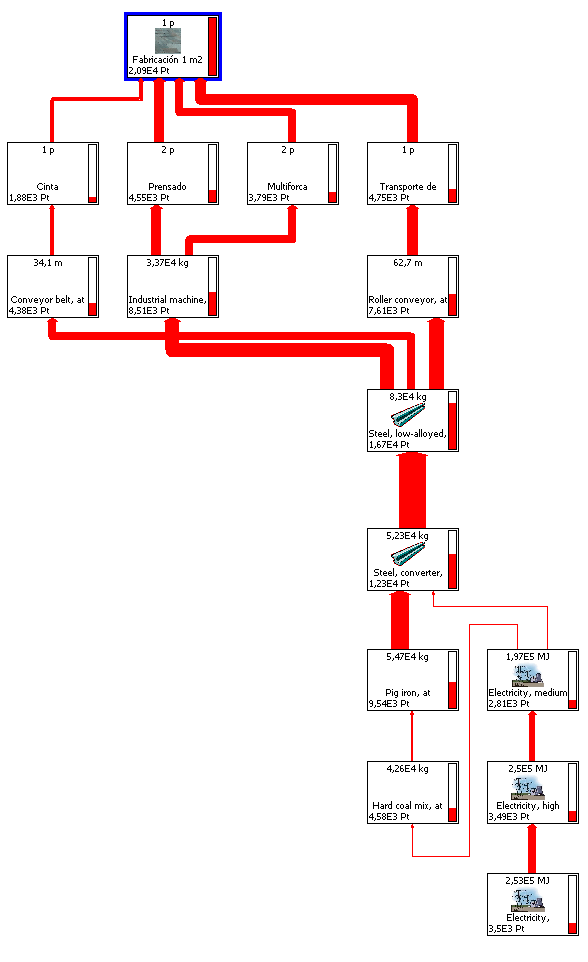
\includegraphics[width=14cm]{img/fabric_red.png}
\caption{Red de la fase de extracción de materias primas, fabricación e instalación.}
\label{fig:fabric_red}
\end{figure}

Cada caja representa un proceso y cada proceso se muestra una única vez. Las flechas representan los flujos entre procesos. Las barras o termómetros indican la carga medioambiental generada en cada proceso y sus procesos aguas arriba. De esta manera se puede distinguir entre los procesos más importantes y los menos, identificando los puntos calientes.

De la red de la fase de extracción de materias primas, fabricación e instalación se puede obtener que la extracción de materias primas para la capa bituminosa y el árido grueso de la capa base de la instalación son los procesos con mayor carga medioambiental de esta fase. También destaca el proceso de fabricación del cemento Portland para la creación del hormigón del adoquín.

La caracterización del análisis de impacto muestra todas las categorías de impacto. Cada una de ellas tiene una unidad de medida diferente, por lo que se representan gráficamente de forma porcentual. Para tener una visión más clara de los impactos relevantes de la fase, es mejor recurrir a la normalización donde las diferentes puntuaciones de los impactos caracterizados se relativizan a una referencia común.

La figura \ref{fig:fabric_normalizacion} y la tabla \ref{categoriasimpactofabricacion} muestran las categorías de impacto relevantes de esta fase.

\begin{figure}[!htb]
\centering
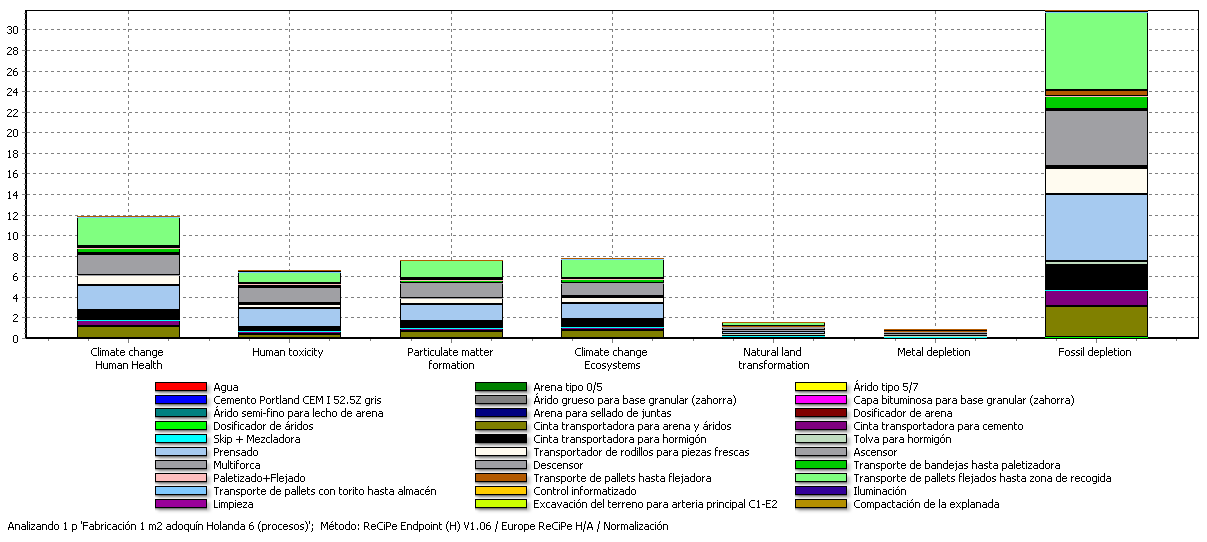
\includegraphics[width=15cm]{img/fabric_normalizacion.png}
\caption{Cuantificación de los impactos normalizados de la fase de extracción de materias primas, fabricación e instalación.}
\label{fig:fabric_normalizacion}
\end{figure}

La categoría con mayor impacto es la de ``Agotamiento de recursos fósiles'', donde destacan la extracción de materias primas para la capa bituminosa y el árido grueso de la capa base de la instalación y el proceso de fabricación del cemento Portland. Para el resto de categorías de impacto se produce una situación similar. En la categoría de ``Ocupación de tierras agrícolas'' presenta cierta relevancia el proceso de paletizado y flejado de los pallets debido a la tala de árboles para la fabricación de madera y papel.

\begin{table}[!htb]
\centering
\begin{tabular}{p{4cm}rrrrrrr}
\toprule
\multicolumn{8}{c}{Categorías de impacto normalizadas}\\
\midrule
Proceso & CC[HH] & HT & PMF & CC[Ec] & ALO & NLT & FD\\
 &  (\%) & (\%) & (\%) & (\%) & (\%) & (\%) & (\%)\\
\midrule
Capa bituminosa para base granular & 23.2 & 17.0 & 16.5 & 23.2 & 3.09 & 30.5 & 55.2\\
Árido grueso para base granular & 26.8 & 28.9 & 46.9 & 26.8 & 65.2 & 35.4 & 21.3\\
Cemento Portland CEM I gris & 27.4 & 9.62 & 8.13 & 27.4 & 0.21 & 1.48 & 6.67\\
Paletizado y flejado & 3.2 & 9.42 & 3.78 & 3.2 & 31.2 & 14.4 & 2.36\\
Sellado y vibrado del pavimento & 4.56 & 0.79 & 8.1 & 4.56 & 0.01 & 2.62 & 3.69\\
\bottomrule
\end{tabular}
\caption[Categorías de impacto normalizadas de la fase de extracción de materias primas, fabricación e instalación.]{Categorías de impacto normalizadas de la fase de extracción de materias primas, fabricación e instalación. CC[HH]: cambio climático—salud humana, HT: toxicidad humana, PMF: formación de partículas, CC[Ec]: cambio climático—ecosistema, ALO: ocupación de tierras agrícolas, NLT: transformación natural de la tierra, FD: agotamiento de recursos fósiles.}
\label{categoriasimpactofabricacion}
\end{table}

La puntuación única permite observar los resultados desde una perspectiva diferente. Esta opción agrupa las categorías de impacto aplicando una serie de puntos a cada una, representando finalmente todas las categorías de impacto usando una misma unidad, el punto (\textit{Point}, Pt). La carga ambiental será mayor cuanto más Pt tenga.

\begin{figure}[!htb]
\centering
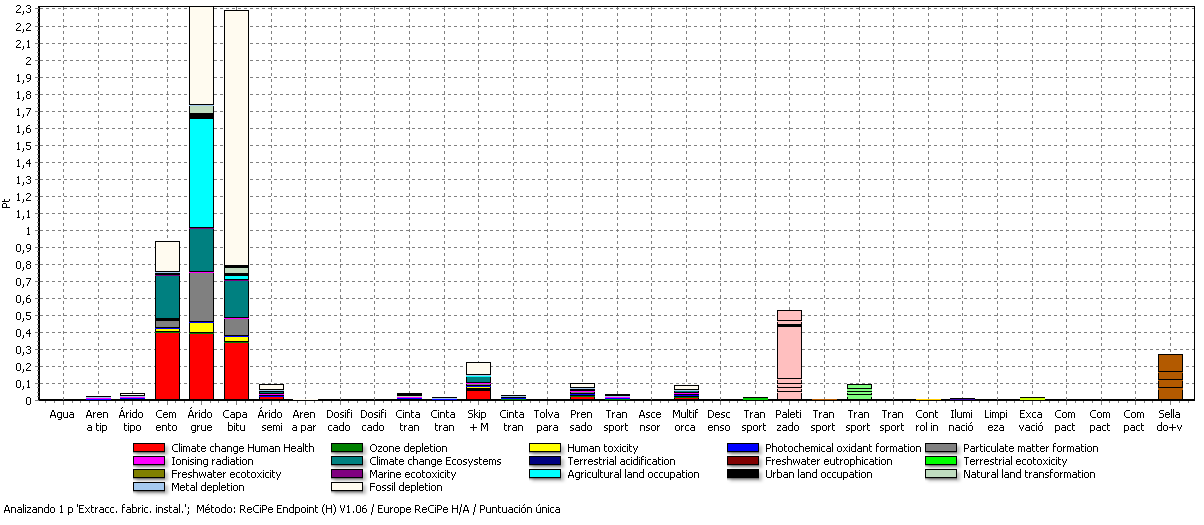
\includegraphics[width=15cm]{img/fabric_puntuacionunica.png}
\caption{Cuantificación de los impactos a nivel de puntuación única de la fase de extracción de materias primas, fabricación e instalación.}
\label{fig:fabric_puntuacionunica}
\end{figure}

La figura \ref{fig:fabric_puntuacionunica} muestra las categorías de impacto a nivel de puntuación única. Los resultados son similares a los de la normalización, donde la extracción de materias primas para la capa bituminosa y el árido grueso de la capa base de la instalación y el proceso de fabricación del cemento Portland tienen la mayor puntuación (ver tabla \ref{categoriasimpactofabricacionpuntunica}).

\begin{table}[!htb]
\centering
\begin{tabular}{p{4cm}rrrrrrr}
\toprule
\multicolumn{8}{c}{Categorías de impacto puntuación final}\\
\midrule
Proceso & CC[HH] & HT & PMF & CC[Ec] & ALO & NLT & FD\\
 &  (\%) & (\%) & (\%) & (\%) & (\%) & (\%) & (\%)\\
\midrule
Capa bituminosa para base granular & 23.2 & 17.0 & 16.5 & 23.2 & 3.09 & 30.5 & 55.2\\
Árido grueso para base granular & 26.8 & 28.9 & 46.9 & 26.8 & 65.2 & 35.4 & 21.3\\
Cemento Portland CEM I gris & 27.4 & 9.62 & 8.13 & 27.4 & 0.21 & 1.48 & 6.67\\
Paletizado y flejado & 3.2 & 9.42 & 3.78 & 3.2 & 31.2 & 14.4 & 2.36\\
Sellado y vibrado del pavimento & 4.56 & 0.79 & 8.1 & 4.56 & 0.01 & 2.62 & 3.69\\
\bottomrule
\end{tabular}
\caption[Categorías de impacto a nivel de puntuación única de la fase de extracción de materias primas, fabricación e instalación.]{Categorías de impacto a nivel de puntuación única de la fase de extracción de materias primas, fabricación e instalación. CC[HH]: cambio climático—salud humana, HT: toxicidad humana, PMF: formación de partículas, CC[Ec]: cambio climático—ecosistema, ALO: ocupación de tierras agrícolas, NLT: transformación natural de la tierra, FD: agotamiento de recursos fósiles.}
\label{categoriasimpactofabricacionpuntunica}
\end{table}

Atendiendo a las categorías de daños (punto final) de la tabla \ref{categoriasdanosfabricacion}, los resultados indican que el mayor daño se produce en el aspecto de recursos.

\begin{table}[!htb]
\centering
\begin{tabular}{p{6cm}rrrr}
\toprule
\multicolumn{5}{c}{Categorías de daño puntuación única}\\
\midrule
Proceso & Salud hum. & Ecosistema & Recursos & Total\\
 & (Pt) & (Pt) &  (Pt) & (Pt)\\
\midrule
Capa bituminosa para base granular & 0.482 & 0.302 & 1.510 & 2.290\\
Árido grueso para base granular & 0.753 & 0.979 & 0.582 & 2.310\\
Cemento Portland CEM I gris & 0.473 & 0.277 & 0.182 & 0.932\\
Paletizado y flejado & 0.093 & 0.370 & 0.065 & 0.527\\
Sellado y vibrado del pavimento & 0.119 & 0.048 & 0.101 & 0.268\\
\midrule
Total (Pt) & 2.32 & 2.15 & 2.74 & \textbf{7.21}\\
\bottomrule
\end{tabular}
\caption{Puntuación única por categorías de daños de la fase de extracción de materias primas, fabricación e instalación.}
\label{categoriasdanosfabricacion}
\end{table}

\section{Evaluación del Impacto Ambiental de la fase de uso y mantenimiento}

La red de la fase de uso y mantenimiento de la figura \ref{fig:uso_red} muestra todos los procesos interrelacionados para dar una perspectiva general de la fase.

\begin{figure}[!htb]
\centering
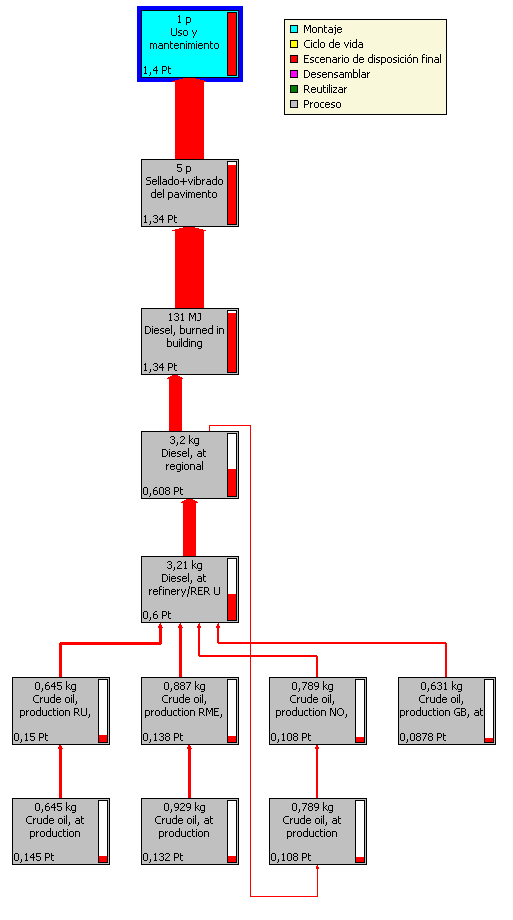
\includegraphics[width=5cm]{img/uso_red.png}
\caption{Red de la fase de uso y mantenimiento.}
\label{fig:uso_red}
\end{figure}

Cada caja representa un proceso y cada proceso se muestra una única vez. Las flechas representan los flujos entre procesos. Las barras o termómetros indican la carga medioambiental generada en cada proceso y sus procesos aguas arriba. De esta manera se puede distinguir entre los procesos más importantes y los menos, identificando los puntos calientes.

Como era de esperar, en la red de la fase de uso y mantenimiento el proceso con mayor carga ambiental es el sellado y vibrado del pavimento.

La caracterización del análisis de impacto muestra todas las categorías de impacto. Cada una de ellas tiene una unidad de medida diferente, por lo que se representan gráficamente de forma porcentual. Para tener una visión más clara de los impactos relevantes de la fase, es mejor recurrir a la normalización donde las diferentes puntuaciones de los impactos caracterizados se relativizan a una referencia común.

La figura \ref{fig:uso_normalizacion} y la tabla \ref{categoriasimpactouso} muestran las categorías de impacto relevantes de esta fase.

\begin{figure}[!htb]
\centering
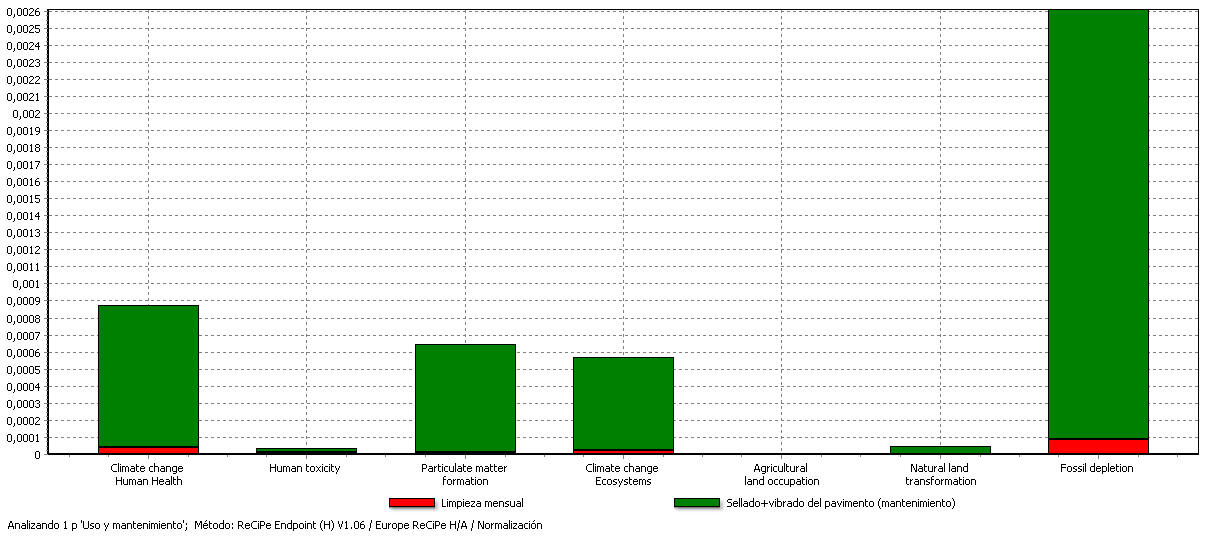
\includegraphics[width=15cm]{img/uso_normalizacion.png}
\caption{Cuantificación de los impactos normalizados de la fase de uso y mantenimiento.}
\label{fig:uso_normalizacion}
\end{figure}

Al igual que en la fase de extracción de materias primas, fabricación e instalación, la categoría con mayor impacto es la de ``Agotamiento de recursos fósiles'', donde el sellado y vibrado del pavimento es el proceso dominante. El resto de categorías de impacto muestran la misma situación.

\begin{table}[!htb]
\centering
\begin{tabular}{p{4cm}rrrrrrr}
\toprule
\multicolumn{8}{c}{Categorías de impacto normalizadas}\\
\midrule
Proceso & CC[HH] & HT & PMF & CC[Ec] & ALO & NLT & FD\\
 &  (\%) & (\%) & (\%) & (\%) & (\%) & (\%) & (\%)\\
\midrule
Limpieza mensual & 4.54 & 38.6 & 1.75 & 4.54 & 71.4 & 3.57 & 3.48\\
Sellado y vibrado & 95.5 & 61.4 & 98.2 & 95.5 & 28.6 & 96.4 & 96.5\\
\bottomrule
\end{tabular}
\caption[Categorías de impacto normalizadas de la fase de uso y mantenimiento.]{Categorías de impacto normalizadas de la fase de uso y mantenimiento. CC[HH]: cambio climático—salud humana, HT: toxicidad humana, PMF: formación de partículas, CC[Ec]: cambio climático—ecosistema, ALO: ocupación de tierras agrícolas, NLT: transformación natural de la tierra, FD: agotamiento de recursos fósiles.}
\label{categoriasimpactouso}
\end{table}

La puntuación única permite observar los resultados desde una perspectiva diferente. Esta opción agrupa las categorías de impacto aplicando una serie de puntos a cada una, representando finalmente todas las categorías de impacto usando una misma unidad, el punto (\textit{Point}, Pt). La carga ambiental será mayor cuanto más Pt tenga.

\begin{figure}[!htb]
\centering
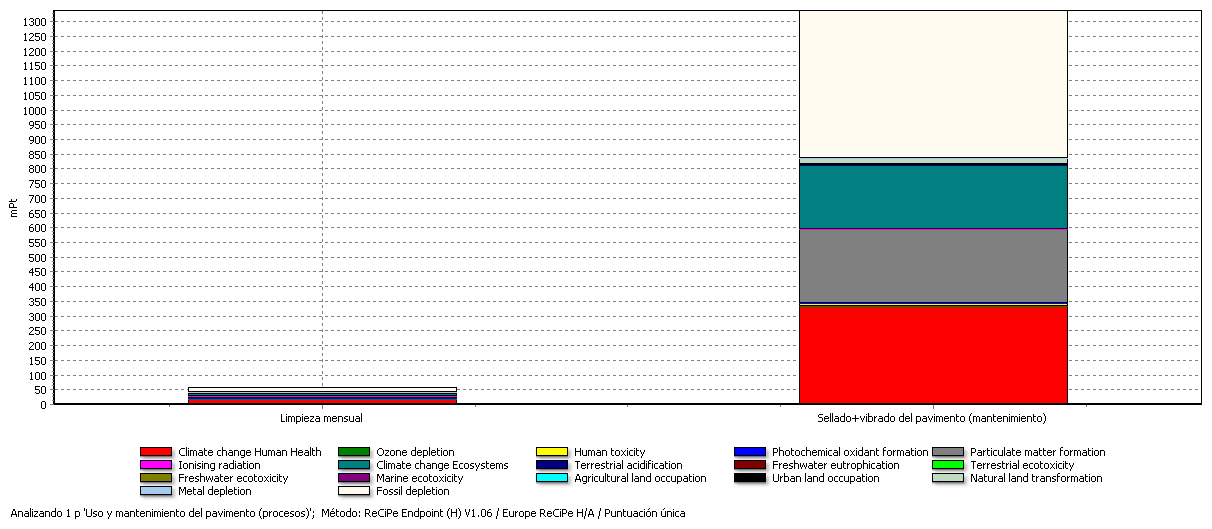
\includegraphics[width=15cm]{img/uso_puntuacionunica.png}
\caption{Cuantificación de los impactos a nivel de puntuación única de uso y mantenimiento.}
\label{fig:uso_puntuacionunica}
\end{figure}

La figura \ref{fig:uso_puntuacionunica} muestra las categorías de impacto a nivel de puntuación única. Los resultados son similares a los de la normalización. El proceso de sellado y vibrado del pavimento afecta principalmente a las categorías de agotamiento de recursos fósiles y al cambio climático desde el punto de vista de la salud humana. En menor medida afecta al cambio climática visto desde el ecosistema y a la formación de partículas (ver tabla \ref{categoriasimpactousopuntunica}).

\begin{table}[!htb]
\centering
\begin{tabular}{p{4cm}rrrrrrr}
\toprule
\multicolumn{8}{c}{Categorías de impacto puntuación única}\\
\midrule
Proceso & CC[HH] & HT & PMF & CC[Ec] & ALO & NLT & FD\\
 &  (\%) & (\%) & (\%) & (\%) & (\%) & (\%) & (\%)\\
\midrule
Limpieza & 4.54 & 38.6 & 1.75 & 4.54 & 54.1 & 3.57 & 3.48\\
Sellado y vibrado & 95.5 & 61.4 & 98.2 & 95.5 & 28.6 & 96.4 & 96.5\\
\bottomrule
\end{tabular}
\caption[Categorías de impacto a nivel de puntuación única de la fase de uso y mantenimiento.]{Categorías de impacto a nivel de puntuación única de la fase de uso y mantenimiento. CC[HH]: cambio climático—salud humana, HT: toxicidad humana, PMF: formación de partículas, CC[Ec]: cambio climático—ecosistema, ALO: ocupación de tierras agrícolas, NLT: transformación natural de la tierra, FD: agotamiento de recursos fósiles.}
\label{categoriasimpactousopuntunica}
\end{table}

Atendiendo a las categorías de daños (punto final) de la tabla \ref{categoriasdanosuso}, los resultados indican que el mayor daño se produce en la salud humana.

\begin{table}[!htb]
\centering
\begin{tabular}{p{6cm}rrrr}
\toprule
\multicolumn{5}{c}{Categorías de daño puntuación única}\\
\midrule
Proceso & Salud hum. & Ecosistema & Recursos & Total\\
 & (Pt) & (Pt) &  (Pt) & (Pt)\\
\midrule
Limpieza & 0.0262 & 0.0134 & 0.0182 & 0.0577\\
Sellado y vibrado & 0.5940 & 0.2400 & 0.5040 & 1.3400\\
\midrule
Total (Pt) & 0.621 & 0.253 & 0.522 & \textbf{1.4}\\
\bottomrule
\end{tabular}
\caption{Puntuación única por categorías de daños de la fase de uso y mantenimiento.}
\label{categoriasdanosuso}
\end{table}

\section{Evaluación del Impacto Ambiental de la fase de fin de vida}

En la red de la fase de fin de vida de la figura \ref{fig:fdv_red} se muestran todos los procesos interrelacionados para dar una perspectiva general de la fase.

\begin{figure}[!htb]
\centering
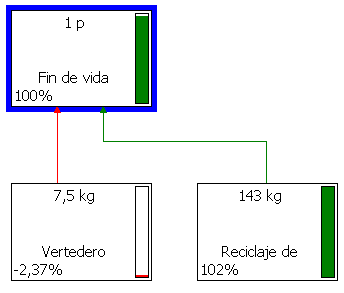
\includegraphics[width=5cm]{img/fdv_red.png}
\caption{Red de la fase de fin de vida.}
\label{fig:fdv_red}
\end{figure}

Cada caja representa un proceso y cada proceso se muestra una única vez. Las flechas representan los flujos entre procesos. Las barras o termómetros indican la carga medioambiental generada en cada proceso y sus procesos aguas arriba. De esta manera se puede distinguir entre los procesos más importantes y los menos, identificando los puntos calientes.

En la red de la fase de fin de vida los procesos se muestran termómetros verdes en lugar de rojos, ya que se tiene en cuenta el beneficio ambiental del proceso de reciclaje del adoquín en árido, por lo que el vertedero tiene un beneficio negativo, es decir un impacto ambiental.

La caracterización del análisis de impacto muestra todas las categorías de impacto. Cada una de ellas tiene una unidad de medida diferente, por lo que se representan gráficamente de forma porcentual. Para tener una visión más clara de los impactos relevantes de la fase, es mejor recurrir a la normalización donde las diferentes puntuaciones de los impactos caracterizados se relativizan a una referencia común.

La figura \ref{fig:fdv_normalizacion} y la tabla \ref{categoriasimpactofdv} muestran las categorías de impacto relevantes de esta fase.

\begin{figure}[!htb]
\centering
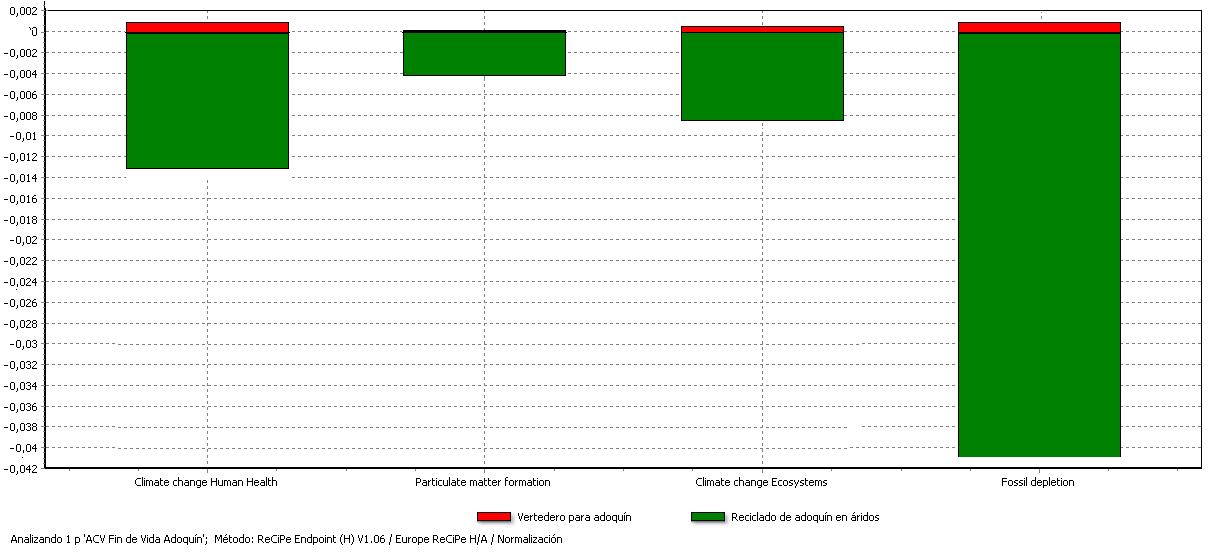
\includegraphics[width=15cm]{img/fdv_normalizacion.png}
\caption{Cuantificación de los impactos normalizados de la fase de fin de vida.}
\label{fig:fdv_normalizacion}
\end{figure}

A diferencia de las dos fases anteriores, se produce un beneficio, principalmente en la categoría de ``Agotamiento de recursos fósiles'', donde el reciclaje de adoquín en árido supone un producto evitado, el árido, cuya carga ambiental es negativa (beneficio ambiental).

\begin{table}[!htb]
\centering
\begin{tabular}{p{4cm}rrrrrrr}
\toprule
\multicolumn{8}{c}{Categorías de impacto normalizadas}\\
\midrule
Proceso & CC[HH] & HT & PMF & CC[Ec] & ALO & NLT & FD\\
 &  (\%) & (\%) & (\%) & (\%) & (\%) & (\%) & (\%)\\
\midrule
Vertedero & 1.65 & 1.01 & 3.51 & 1.65 & 6.88 & -10.6 & 4.52\\
Reciclaje de adoquín en árido & -102 & -101 & -104 & -102 & -07 & -89.4 & -105\\
\bottomrule
\end{tabular}
\caption[Categorías de impacto normalizadas de la fase de fin de vida.]{Categorías de impacto normalizadas de la fase de fin de vida. CC[HH]: cambio climático—salud humana, HT: toxicidad humana, PMF: formación de partículas, CC[Ec]: cambio climático—ecosistema, ALO: ocupación de tierras agrícolas, NLT: transformación natural de la tierra, FD: agotamiento de recursos fósiles.}
\label{categoriasimpactofdv}
\end{table}

La puntuación única permite observar los resultados desde una perspectiva diferente. Esta opción agrupa las categorías de impacto aplicando una serie de puntos a cada una, representando finalmente todas las categorías de impacto usando una misma unidad, el kilopunto (\textit{kiloPoint}, kPt). La carga ambiental será mayor cuanto más kPt tenga.

\begin{figure}[!htb]
\centering
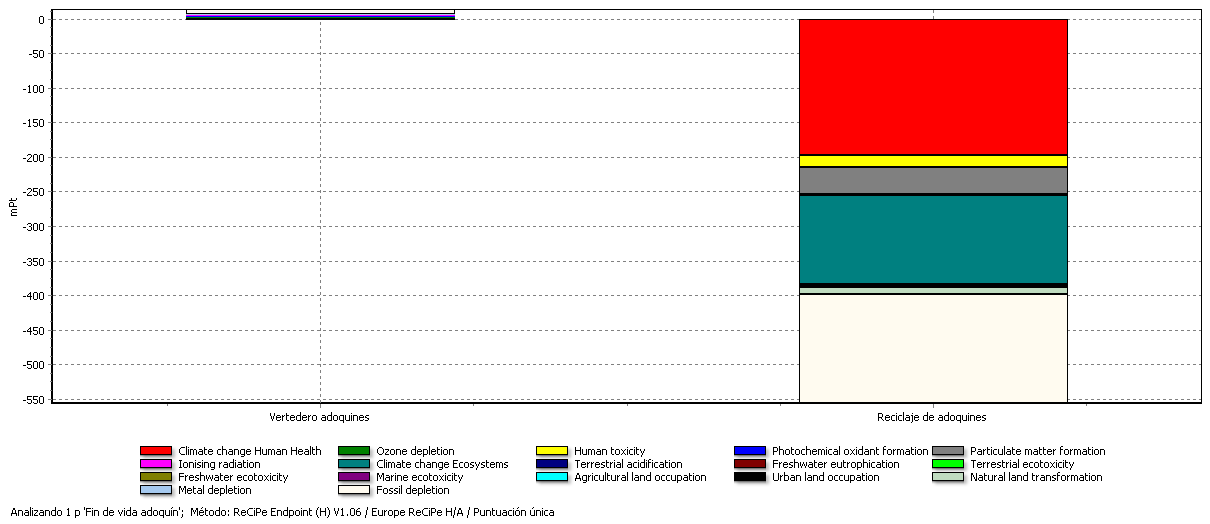
\includegraphics[width=15cm]{img/fdv_puntuacionunica.png}
\caption{Cuantificación de los impactos a nivel de puntuación única de fin de vida.}
\label{fig:fdv_puntuacionunica}
\end{figure}

La figura \ref{fig:fdv_puntuacionunica} muestra las categorías de impacto a nivel de puntuación única. Los resultados son coherentes con los de la normalización. El proceso de reciclaje de adoquín en áridos aporta un beneficio principalmente a las categorías de agotamiento de recursos fósiles y al cambio climático desde el punto de vista de la salud humana. También beneficia, en menor proporción, al cambio climática visto desde el ecosistema y a la formación de partículas (ver tabla \ref{categoriasimpactofdvpuntunica}).

\begin{table}[!htb]
\centering
\begin{tabular}{p{4cm}rrrrrrr}
\toprule
\multicolumn{8}{c}{Categorías de impacto puntuación única}\\
\midrule
Proceso & CC[HH] & HT & PMF & CC[Ec] & ALO & NLT & FD\\
 &  (\%) & (\%) & (\%) & (\%) & (\%) & (\%) & (\%)\\
\midrule
Vertedero & 1.65 & 1.01 & 3.51 & 1.65 & 6.88 & -10.6 & 4.52\\
Reciclaje de adoquín en árido & -102 & -101 & -104 & -102 & -07 & -89.4 & -105\\
\bottomrule
\end{tabular}
\caption[Categorías de impacto a nivel de puntuación única de la fase de fin de vida.]{Categorías de impacto a nivel de puntuación única de la fase de fin de vida. CC[HH]: cambio climático—salud humana, HT: toxicidad humana, PMF: formación de partículas, CC[Ec]: cambio climático—ecosistema, ALO: ocupación de tierras agrícolas, NLT: transformación natural de la tierra, FD: agotamiento de recursos fósiles.}
\label{categoriasimpactofdvpuntunica}
\end{table}

Atendiendo a las categorías de daños (punto final) de la tabla \ref{categoriasdanosfdv}, los resultados indican que el mayor beneficio se produce en el aspecto de recursos.

\begin{table}[!htb]
\centering
\begin{tabular}{p{6cm}rrrr}
\toprule
\multicolumn{5}{c}{Categorías de daño puntuación única}\\
\midrule
Proceso & Salud hum. & Ecosistema & Recursos & Total\\
 & (Pt) & (Pt) & (Pt) & (Pt)\\
\midrule
Vertedero & 0.00473 & 0.00136 & 0.00681 & 0.0129\\
Reciclaje de adoquín en árido & -0.255 & -0.143 & -0.158 & -0.556\\
\midrule
Total (Pt) & -0.251 & -0.142 & -0.151 & \textbf{-0.543}\\
\bottomrule
\end{tabular}
\caption{Categorías de daños de la fase de fin de vida.}
\label{categoriasdanosfdv}
\end{table}

\section{Evaluación del Impacto Ambiental del ciclo de vida completo}

Una vez estudiadas las tres fases del ciclo de vida se procederá a realizar un análisis completo del producto a lo largo de las tres fases anteriores de su ciclo de vida.

A priori, observando los resultados ya obtenidos en las tablas de categorías de impacto \ref{categoriasimpactofabricacion}, \ref{categoriasimpactouso} y \ref{categoriasimpactofdv}, se puede asegurar que las etapas de uso y mantenimiento y fin de vida tienen menores consecuencias comparadas con la de extracción de materias primas, fabricación e instalación.

La red del ciclo de vida completo de la figura \ref{fig:completo_red} demuestra que la únicamente la fase de extracción de materias primas, fabricación e instalación representa un impacto del 89.4\%, mientras que la de uso y mantenimiento aporta un 17.3\% y la de fin de vida un beneficio del 6.74\%.

\begin{figure}[!htb]
\centering
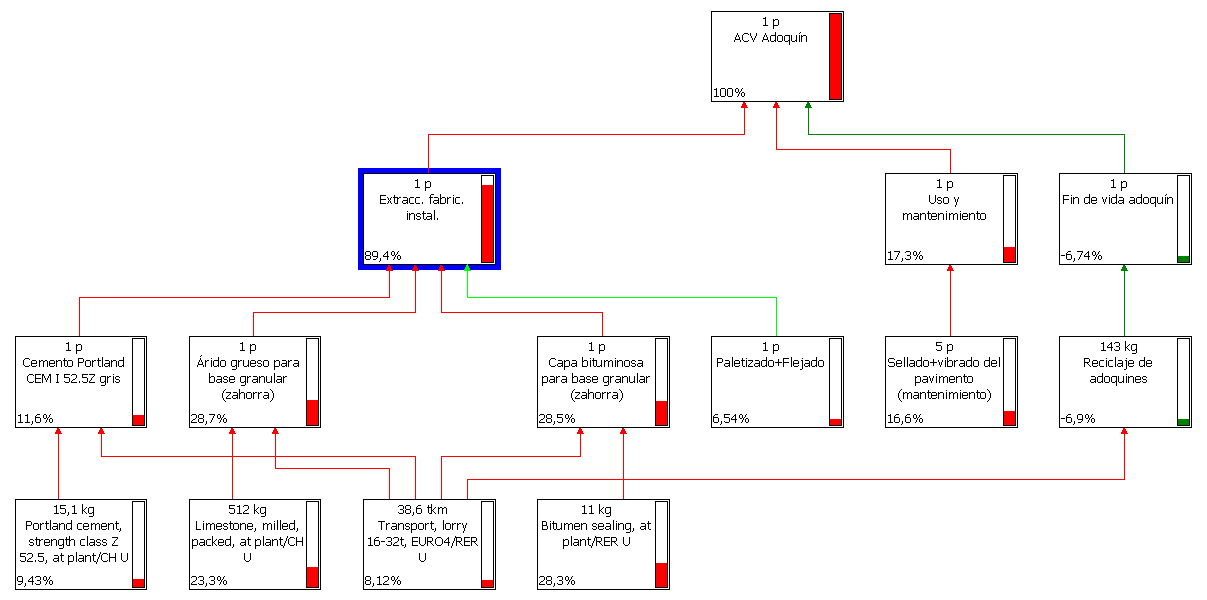
\includegraphics[width=14cm]{img/completo_red.png}
\caption{Red del ciclo de vida completo.}
\label{fig:completo_red}
\end{figure}

Cada caja representa un proceso y cada proceso se muestra una única vez. Las flechas representan los flujos entre procesos. Las barras o termómetros indican la carga medioambiental generada en cada proceso y sus procesos aguas arriba. Si el termómetro es de color verde indica que es un beneficio ambiental. De esta manera se puede distinguir entre los procesos más importantes y los menos, identificando los puntos calientes.

La caracterización del análisis de impacto de la figura \ref{fig:completo_caracterizacion} y la tabla \ref{categoriasimpactocompletocaracterizados} muestra todas las categorías de impacto. Cada una de ellas tiene una unidad de medida diferente, por lo que se representan de forma porcentual.

\begin{figure}[!htb]
\centering
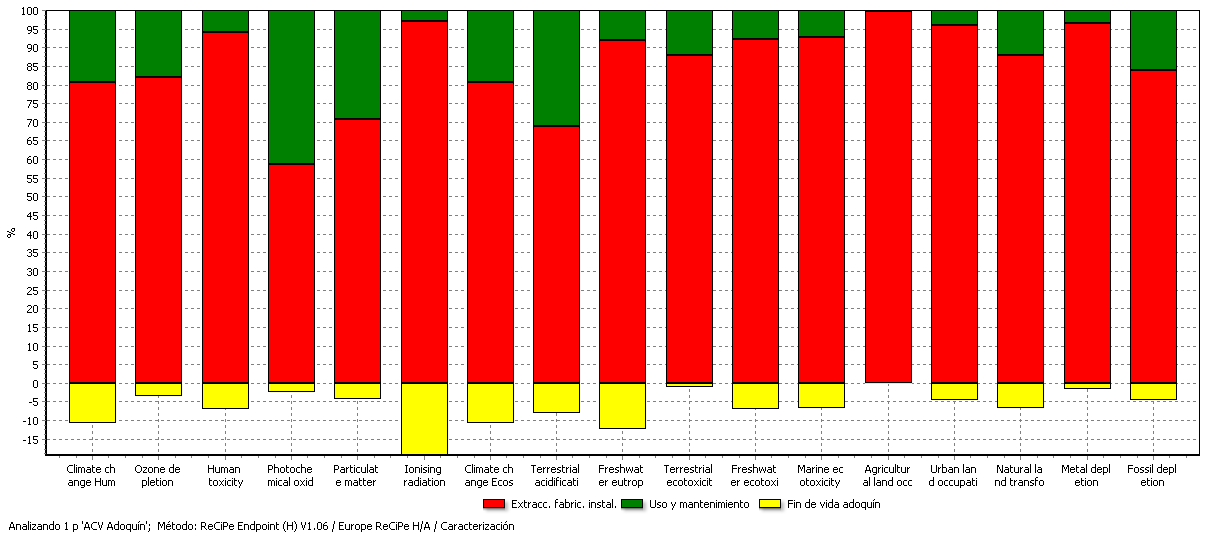
\includegraphics[width=15cm]{img/completo_caracterizacion.png}
\caption{Cuantificación de los impactos caracterizados del ciclo de vida completo.}
\label{fig:completo_caracterizacion}
\end{figure}

\begin{table}[!htb]
\centering
\begin{tabular}{p{2cm}rrrrrrrrr}
\toprule
\multicolumn{10}{c}{Categorías de impacto caracterizadas}\\
\midrule
Proceso & CC[HH] & OD & HT & POF & PMF & IR & CC[Ec] & TA & FE\\
 &  (\%) & (\%) & (\%) & (\%) & (\%) & (\%) & (\%) & (\%) & (\%)\\
\midrule
Ex-fab-inst. & 90.4 & 85.1 & 101 & 60.1 & 74 & 120 & 90.4 & 75.1& 105\\
Uso-mant. & 21.6 & 18.6 & 6.46 & 42.3 & 30.5 & 3.71 & 21.6 & 33.9 & 9.18\\
Fin-vida & -12 & -3.72 & -7.45 & -2.47 & -4.56 & -24 & -12 & -8.93 & -14\\
\midrule
\midrule
Proceso & TE & FE & ME & ALO & ULO & NLT & MD & FD\\
 &  (\%) & (\%) & (\%) & (\%) & (\%) & (\%) & (\%) & (\%)\\
\midrule
Ex-fab-inst. & 88.8 & 99.4 & 99.4 & 100 & 100 & 94.4 & 98.1 & 88\\
Uso-mant. & 12.2 & 8.25 & 7.74 & 0.14 & 4.32 & 12.8 & 3.66 & 16.8\\
Fin-vida & -1.01 & -7.65 & -7.18 & -0.09 & -4.78 & -7.21 & -1.74 & -4.85\\
\bottomrule
\end{tabular}
\caption[Categorías de impacto caracterizadas del ciclo de vida completo.]{Categorías de impacto caracterizadas del ciclo de vida completo. CC[HH]: cambio climático—salud humana, OD: Agotamiento de ozono, HT: toxicidad humana, POF: formación de oxidantes fotoquímicos, PMF: formación de partículas, IR: radiaciones ionizantes, CC[Ec]: cambio climático—ecosistema, TA: acidificación terrestre, FE: eutrofización del agua dulce, TE: ecotoxicidad terrestre, FE: ecotoxicidad del agua dulce, ME: ecotoxicidad marina, ALO: ocupación de tierras agrícolas, ULO: ocupación de suelo urbano, NLT: transformación natural de la tierra, MD: agotamiento de recursos minerales, FD: agotamiento de recursos fósiles.}
\label{categoriasimpactocompletocaracterizados}
\end{table}

Para tener una visión más clara de los impactos relevantes de la fase, es mejor recurrir a la normalización donde las diferentes puntuaciones de los impactos caracterizados se relativizan a una referencia común.

La figura \ref{fig:completo_normalizacion} y la tabla \ref{categoriasimpactocompleto} muestran las categorías de impacto relevantes de esta fase.

\begin{figure}[!htb]
\centering
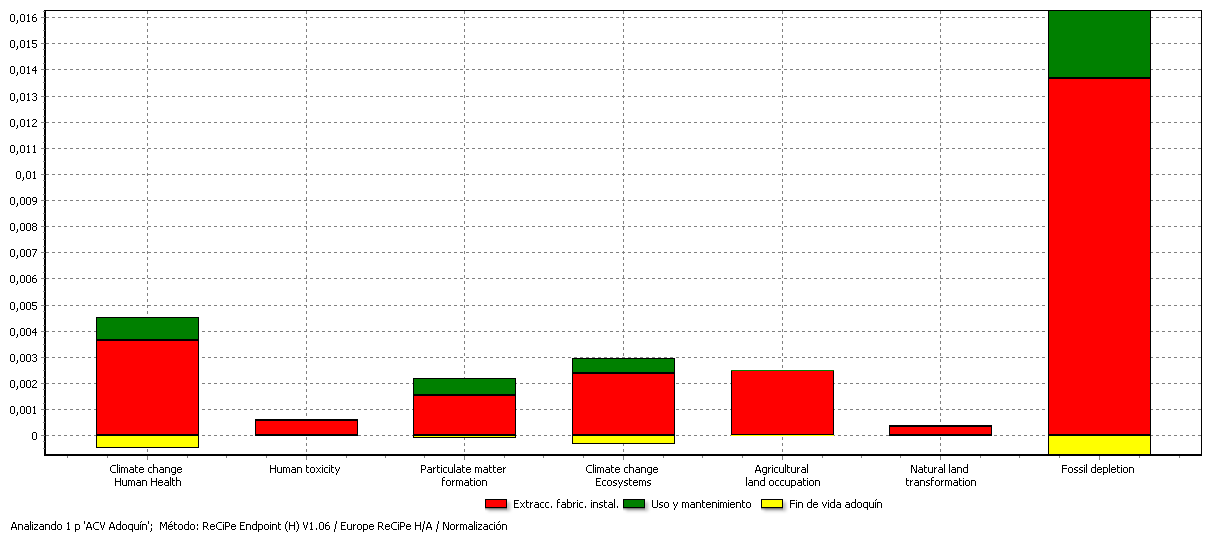
\includegraphics[width=15cm]{img/completo_normalizacion.png}
\caption{Cuantificación de los impactos normalizados del ciclo de vida completo.}
\label{fig:completo_normalizacion}
\end{figure}

La categoría con mayor impacto es la de ``Agotamiento de recursos fósiles'', donde la fase que predomina es la de extracción de materias primas, fabricación e instalación en todas las categorías de impacto (ver figura \ref{fig:completo_normalizacion}).

\begin{table}[!htb]
\centering
\begin{tabular}{p{4cm}rrrrrrr}
\toprule
\multicolumn{8}{c}{Categorías de impacto normalizadas}\\
\midrule
Proceso & CC[HH] & HT & PMF & CC[Ec] & ALO & NLT & FD\\
 &  (\%) & (\%) & (\%) & (\%) & (\%) & (\%) & (\%)\\
\midrule
Extracc., fabric. e instal. & 90.4 & 101 & 74 & 90.4 & 100 & 94.4 & 88\\
Uso y mantenim. & 21.6 & 6.46 & 30.5 & 21.6 & 0.14 & 12.8 & 16.8\\
Fin de vida & -12 & -7.45 & -4.56 & -12 & -0.09 & -7.21 & -4.85\\
\bottomrule
\end{tabular}
\caption[Categorías de impacto normalizadas del ciclo de vida completo.]{Categorías de impacto normalizadas del ciclo de vida completo. CC[HH]: cambio climático—salud humana, HT: toxicidad humana, PMF: formación de partículas, CC[Ec]: cambio climático—ecosistema, ALO: ocupación de tierras agrícolas, NLT: transformación natural de la tierra, FD: agotamiento de recursos fósiles.}
\label{categoriasimpactocompleto}
\end{table}

Los datos ponderados de la tabla \ref{categoriasimpactocompletoponderados} indican resultados similares a la normalización.

\begin{table}[!htb]
\centering
\begin{tabular}{p{4cm}rrrrrrr}
\toprule
\multicolumn{8}{c}{Categorías de impacto ponderadas}\\
\midrule
Proceso & CC[HH] & HT & PMF & CC[Ec] & ALO & NLT & FD\\
 &  (\%) & (\%) & (\%) & (\%) & (\%) & (\%) & (\%)\\
\midrule
Extracc., fabric. e instal. & 90.4 & 101 & 74 & 90.4 & 100 & 94.4 & 88\\
Uso y mantenim. & 21.6 & 6.46 & 30.5 & 21.6 & 0.14 & 12.8 & 16.8\\
Fin de vida & -12 & -7.45 & -4.56 & -12 & -0.09 & -7.21 & -4.85\\
\bottomrule
\end{tabular}
\caption[Categorías de impacto ponderadas del ciclo de vida completo.]{Categorías de impacto ponderadas del ciclo de vida completo. CC[HH]: cambio climático—salud humana, HT: toxicidad humana, PMF: formación de partículas, CC[Ec]: cambio climático—ecosistema, ALO: ocupación de tierras agrícolas, NLT: transformación natural de la tierra, FD: agotamiento de recursos fósiles.}
\label{categoriasimpactocompletoponderados}
\end{table}

La puntuación única permite observar los resultados desde una perspectiva diferente. Esta opción agrupa las categorías de impacto aplicando una serie de puntos a cada una, representando finalmente todas las categorías de impacto usando una misma unidad, el punto (\textit{Point}, Pt). La carga ambiental será mayor cuanto más Pt tenga.

\begin{figure}[!htb]
\centering
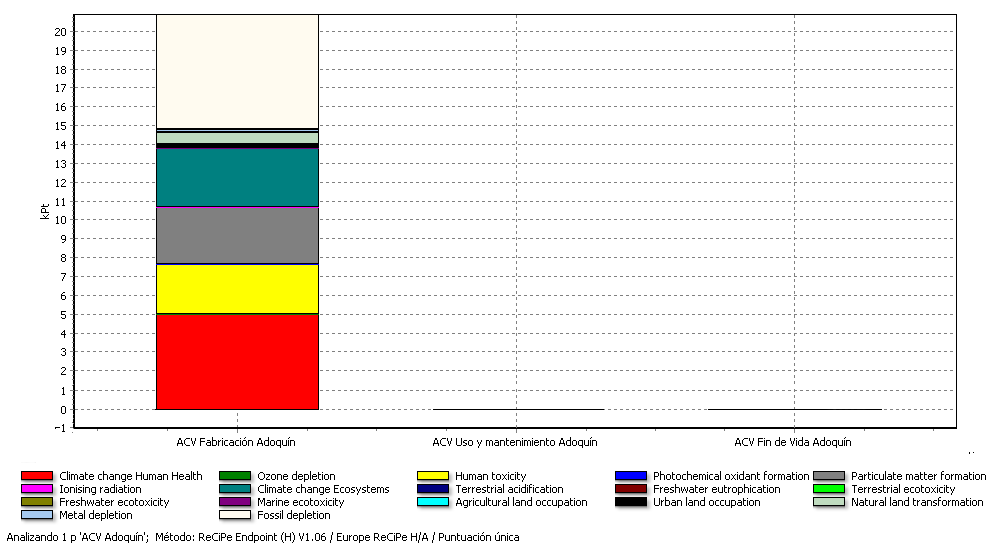
\includegraphics[width=15cm]{img/completo_puntuacionunica.png}
\caption{Cuantificación de los impactos a nivel de puntuación única del ciclo de vida completo.}
\label{fig:completo_puntuacionunica}
\end{figure}

La figura \ref{fig:completo_puntuacionunica} muestra las categorías de impacto a nivel de puntuación única. Los resultados son similares a los de la normalización, donde la fase de extracción de materias primas, fabricación e instalación tiene la mayor puntuación (ver tabla \ref{categoriasimpactocompletopuntunica}).

\begin{table}[!htb]
\centering
\begin{tabular}{p{4cm}rrrrrrr}
\toprule
\multicolumn{8}{c}{Categorías de impacto puntuación única}\\
\midrule
Proceso & CC[HH] & HT & PMF & CC[Ec] & ALO & NLT & FD\\
 &  (\%) & (\%) & (\%) & (\%) & (\%) & (\%) & (\%)\\
\midrule
Extracc., fabric. e instal. & 90.4 & 101 & 74 & 90.4 & 100 & 94.4 & 88\\
Uso y mantenim. & 21.6 & 6.46 & 30.5 & 21.6 & 0.14 & 12.8 & 16.8\\
Fin de vida & -12 & -7.45 & -4.56 & -12 & -0.09 & -7.21 & -4.85\\
\bottomrule
\end{tabular}
\caption[Categorías de impacto a nivel de puntuación única del ciclo de vida completo.]{Categorías de impacto a nivel de puntuación única del ciclo de vida completo. CC[HH]: cambio climático—salud humana, HT: toxicidad humana, PMF: formación de partículas, CC[Ec]: cambio climático—ecosistema, ALO: ocupación de tierras agrícolas, NLT: transformación natural de la tierra, FD: agotamiento de recursos fósiles.}
\label{categoriasimpactocompletopuntunica}
\end{table}

Atendiendo a las categorías de daños (punto final) de la tabla \ref{categoriasdanoscompleto}, los resultados indican que el mayor daño se produce en la salud humana.

\begin{table}[!htb]
\centering
\begin{tabular}{p{6cm}rrrr}
\toprule
\multicolumn{5}{c}{Categorías de daño puntuación única}\\
\midrule
Proceso & Salud hum. & Ecosistema & Recursos & Total\\
 & (Pt) & (Pt) &  (Pt) & (Pt)\\
\midrule
Extracc., fabric. e instal. & 2.32 & 2.15 & 2.74 & 7.21\\
Uso y mantenim. & 0.621 & 0.253 & 0.522 & 1.4\\
Fin de vida & -0.251 & -0.142 & -0.151 & -0.543\\
\midrule
Total (Pt) & 2.69 & 2.26 & 3.11 & \textbf{8.06}\\
\bottomrule
\end{tabular}
\caption{Puntuación única por categorías de daños del ciclo de vida completo.}
\label{categoriasdanoscompleto}
\end{table}

De las tablas \ref{categoriasimpactocompleto}, \ref{categoriasimpactocompletoponderados} y \ref{categoriasimpactocompletopuntunica} se puede extraer la conclusión de que la fase que más contribuye al perfil ambiental del adoquín es la de extracción de materias primas, fabricación e instalación. La fase de uso y mantenimiento contribuye lo suficiente como para despreciarla. Por último, la fase de fin de vida aunque contribuye mínimamente, es necesario tenerla en cuenta para cumplir con la Directiva Europea 1999/31/CE relativa al vertido de residuos.

\subsection{Demanda de Energía Acumulada}
A continuación se realizará un análisis de con el método de cálculo de \textbf{Demanda de Energía Acumulada} para conocer la energía que se consume en cada etapa.

La red de la fase de extracción de materias primas, fabricación e instalación de la figura \ref{fig:ced_red} muestra todos los procesos interrelacionados para dar una perspectiva general de la fase.

\begin{figure}[!htbp]
\centering
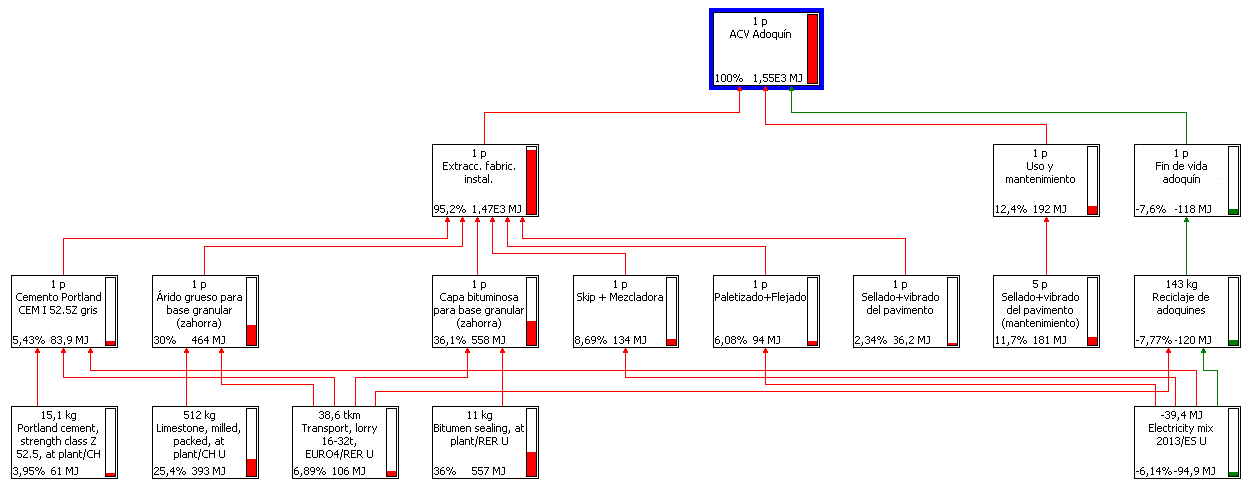
\includegraphics[angle=90,height=18cm]{img/ced_red.png}
\caption{Red del ciclo de vida completo con el método CED.}
\label{fig:ced_red}
\end{figure}

Cada caja representa un proceso y cada proceso se muestra una única vez. Las flechas representan los flujos entre procesos. Las barras o termómetros indican la carga medioambiental generada en cada proceso y sus procesos aguas arriba. De esta manera se puede distinguir entre los procesos más importantes y los menos, identificando los puntos calientes.

La figura \ref{fig:ced_puntuacionunica} y la tabla \ref{tiposenergiaced} muestran que existe el mayor consumo de energía se produce en la fase de extracción de materias primas, fabricación e instalación, suponiendo un total del 95.2\% de toda la vida del producto. Por tanto, es esta fase donde hay que mejorar el consumo y en consecuencia su perfil ambiental.

\begin{figure}[!htb]
\centering
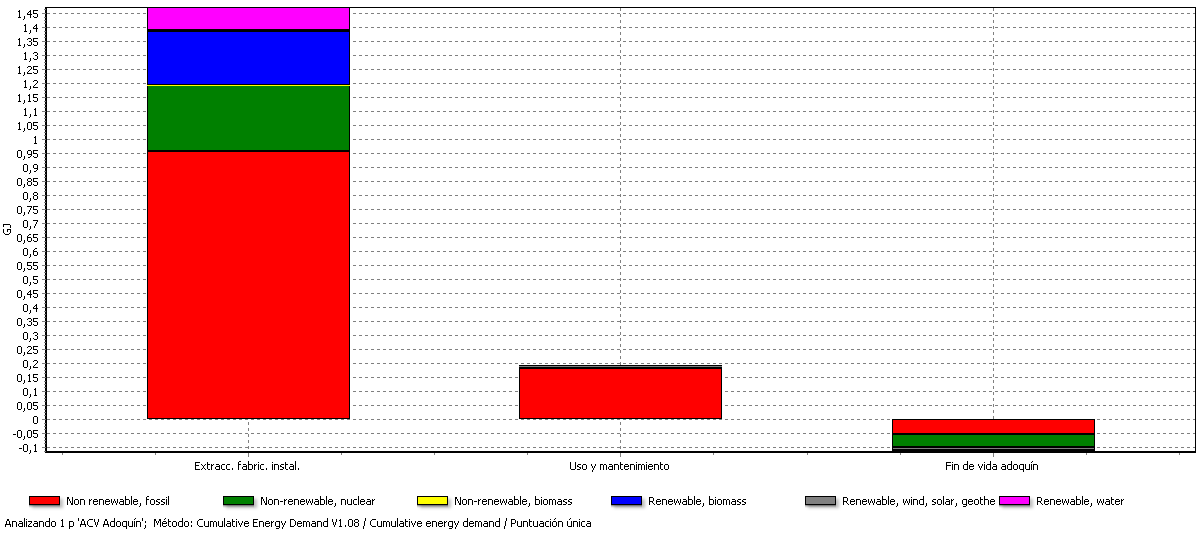
\includegraphics[width=15cm]{img/ced_puntuacionunica.png}
\caption{Cuantificación de los impactos a nivel de puntuación única CED en cada fase.}
\label{fig:ced_puntuacionunica}
\end{figure}

\begin{table}[!htb]
\centering
\begin{tabular}{p{2cm}rrrrrrr}
\toprule
\multicolumn{8}{c}{Tipos de energía consumidos}\\
\midrule
 & \multicolumn{3}{c}{No renovables} & \multicolumn{3}{c}{Renovables}\\
\midrule
Etapa & Fósil & Nuclear & Biom. & Biom. & Viento, sol,& Agua\\
 & (\%) & (\%) & (\%) & (\%) & geo (\%) & (\%)\\
\midrule
Ex-fab-inst. & 88 & 120 & 99.7 & 99.8 & 54 & 111\\
Uso-mant. & 16.8 & 3.66 & 0.53 & 0.39 & 2.22 & 1.24\\
Fin-vida & -4.84 & -23.9 & -0.26 & -0.17 & -156 & -12.1\\
\midrule
\midrule
Etapa & Fósil & Nuclear & Biom. & Biom. & Viento, sol,& Agua & Total\\
& (\si{MJ}) & (\si{MJ}) & (\si{MJ}) & (\si{MJ}) & geo (\si{MJ}) & (\si{MJ}) & (\si{MJ})\\
\midrule
Ex-fab-inst. & 958 & 234 & 0.045 & 196 & 3.18 & 80.9 & 1280\\
Uso-mant. & 183 & 7.11 & 0.001 & 0.77 & 0.13 & 0.90 & 192\\
Fin-vida & -52.6 & -46.5 & -0.001 & -0.325 & -9.2 & -8.84 & -118\\
\midrule
Total (\si{MJ}) & 1040 & 176 & 0.024 & 70.2 & -6.11 & 65-2 & \textbf{1350}\\
\bottomrule
\end{tabular}
\caption{Tipos de energía consumidos en cada fase.}
\label{tiposenergiaced}
\end{table}

La fase de fin de vida aporta un pequeño beneficio del 7.6\% de la energía total consumida en la vida del producto.

\subsection{Cálculo del Potencial de Calentamiento Global}
Finalmente, se utiliza el método IPCC para el cálculo potencial del calentamiento global a lo largo del ciclo de vida. Se aplicará un horizonte temporal a 100 años (GWP 100a) para conocer los kilogramos de \ce{CO2} equivalente que genera el producto en base a la Unidad Funcional (ver tabla \ref{co2generado}).

\begin{table}[!htb]
\centering
\begin{tabular}{p{6cm}rr}
\toprule
\multicolumn{3}{c}{Generación de \ce{CO2}}\\
\midrule
Etapa & IPCC GWP 100a & IPCC GWP 100a\\
 & (\si{kg}\ce{CO2} eq.) & (\%)\\
\midrule
Extracc., fabric. e instal. & 52.5 & 90.4\\
Uso y mantenim. & 12.5 & 21.6\\
Fin de vida & -6.97 & -12\\
\midrule
Total (\si{kg} \ce{CO2} eq.) & \textbf{58.1} & 100\\
\bottomrule
\end{tabular}
\caption{IPCC 2007 GWP 100a: kilogramos de \protect\ce{CO2} equivalente generados en cada fase.}
\label{co2generado}
\end{table}

%!TEX root = informe.tex
\chapter{Análisis de Ciclo de Vida de un adoquín: interpretación}\label{cap:acv_interpretacion}

En la fase de interpretación del ACV los resultados del ICV y del EICV son interpretados de acuerdo al objetivo y alcance marcados inicialmente. En esta fase se realiza un análisis de los resultados y se marcan las conclusiones.

\section{Verificación del análisis de integridad}

El objetivo de esta verificación es ``asegurar que toda la información y datos pertinentes necesarios para la interpretación están disponibles y completos'' \cite{iso14044}. La integridad asegura que no se ha olvidado ningún aspecto importante conocido.

Se ha verificado todos los procesos unitarios de todas las fases, comprobando las entradas/salidas, energía, transporte y residuos.

\section{Verificación del análisis de sensibilidad}

Hasta ahora, para calcular el perfil ambiental se ha utilizado el método ReCiPe desde la perspectiva jerárquica H. Para realizar un análisis de sensibilidad se compararán por fases los resultados con las otras perspectivas mencionadas en la sección \ref{sec:catimpactos}, la individualista (I) y la igualitaria (E).

La figura \ref{fig:sensibilidad_ia_puntuacionunica} y la tabla \ref{sensibilidad_ia_puntuacionunica} muestran los resultados usando la perspectiva individualista (I).

\begin{figure}[!htb]
\centering
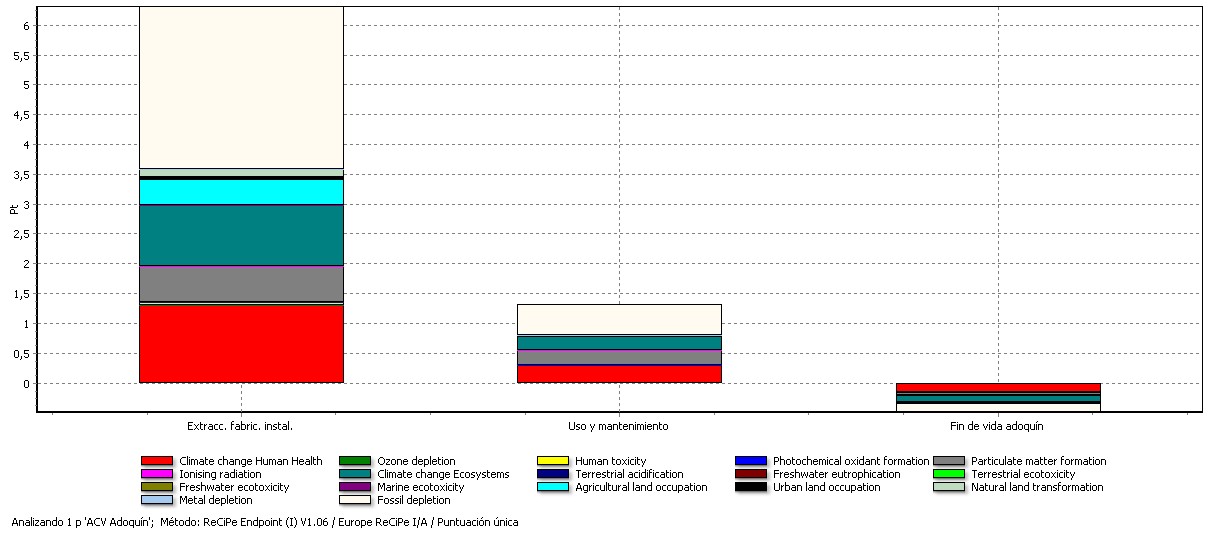
\includegraphics[width=15cm]{img/sensibilidad_ia_puntuacionunica.png}
\caption[Puntuación única por categorías de daño con el método ReCiPe I/A.]{Puntuación única por categorías de daño con el método ReCiPe I/A. Fuente: elaboración propia.}
\label{fig:sensibilidad_ia_puntuacionunica}
\end{figure}

\begin{table}[!htb]
\centering
\begin{tabular}{p{6cm}rrrr}
\toprule
\multicolumn{5}{c}{Categorías de daño puntuación única ReCiPe I/A}\\
\midrule
Etapa & Salud hum. & Ecosistema & Recursos & Total\\
 & (Pt) & (Pt) & (Pt) & (Pt)\\
\midrule
Extracc., fabric. e instal. & 1.96 & 1.61 & 2.74 & 6.31\\
Uso y mantenim. & 0.55 & 0.25 & 0.52 & 1.31\\
Fin de vida & -0.20 & -0.14 & -0.15 & -0.49\\
\bottomrule
\end{tabular}
\caption[Puntuación única por categorías de daño con el método ReCiPe I/A.]{Puntuación única por categorías de daño con el método ReCiPe I/A. Fuente: elaboración propia.}
\label{sensibilidad_ia_puntuacionunica}
\end{table}

La figura \ref{fig:sensibilidad_ia_puntuacionunica} y la tabla \ref{sensibilidad_ia_puntuacionunica} muestran los resultados usando la perspectiva individualista (I).

Por otro lado, la figura \ref{fig:sensibilidad_ea_puntuacionunica} y la tabla \ref{sensibilidad_ea_puntuacionunica} muestran los resultados usando la perspectiva igualitaria (E).

\begin{figure}[!htb]
\centering
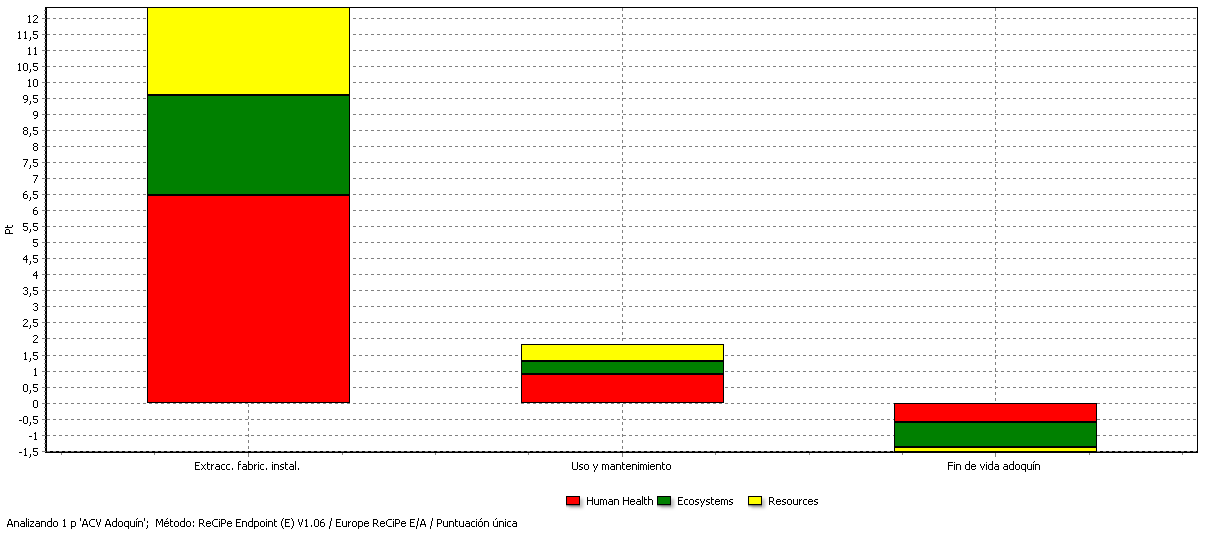
\includegraphics[width=15cm]{img/sensibilidad_ea_puntuacionunica.png}
\caption[Puntuación única por categorías de daño con el método ReCiPe E/A.]{Puntuación única por categorías de daño con el método ReCiPe E/A. Fuente: elaboración propia.}
\label{fig:sensibilidad_ea_puntuacionunica}
\end{figure}

\begin{table}[!htb]
\centering
\begin{tabular}{p{6cm}rrrr}
\toprule
\multicolumn{5}{c}{Categorías de daño puntuación única ReCiPe E/A}\\
\midrule
Etapa & Salud hum. & Ecosistema & Recursos & Total\\
 & (Pt) & (Pt) & (Pt) & (Pt)\\
\midrule
Extracc., fabric. e instal. & 6.46 & 3.13 & 2.74 & 12.3\\
Uso y mantenim. & 0.88 & 0.44 & 0.52 & 1.83\\
Fin de vida & -0.59 & -0.79 & -0.15 & -1.54\\
\bottomrule
\end{tabular}
\caption[Puntuación única por categorías de daño con el método ReCiPe E/A.]{Puntuación única por categorías de daño con el método ReCiPe E/A. Fuente: elaboración propia.}
\label{sensibilidad_ea_puntuacionunica}
\end{table}

La comparación de los resultados entre las tres perspectivas de la tabla \ref{comparativa_perspectivas} indica que las perspectivas jerárquicas e individualista tienen resultados similares, mientras que la igualitaria se diferencia bastante. Mientras que la perspectiva individualista es a corto plazo y optimista en cuanto a que la tecnología puede evitar muchos problemas en el futuro, la perspectiva igualitaria se basa a largo plazo y en una forma de pensar precavida, considerando a la naturaleza frágil e inestable, una visión fatalista poco aceptada, por lo que podría ser descartada para este proyecto, y aceptar esta parte del análisis de sensibilidad como superado.

\begin{table}[!htb]
\centering
\begin{tabular}{p{6cm}rrr}
\toprule
\multicolumn{4}{c}{Comparativa de perspectivas}\\
\midrule
Etapa & I/A & H/A & E/A\\
 & (Pt) & (Pt) & (Pt)\\
\midrule
Extracc., fabric. e instal. & 6.31 & 7.21 & 12.3\\
Uso y mantenim. & 1.31 & 1.4 & 1.83\\
Fin de vida & -0.49 & -0.543 & -1.54\\
\bottomrule
\end{tabular}
\caption[Comparativa de perspectivas I, H, E a nivel del puntuación única por categorías de daño con el método ReCiPe.]{Comparativa de perspectivas I, H, E a nivel del puntuación única por categorías de daño con el método ReCiPe. Fuente: elaboración propia.}
\label{comparativa_perspectivas}
\end{table}

El análisis de sensibilidad necesita además un análisis de incertidumbre utilizando el método ReCiPe H/A con el ``Análisis Monte Carlo''. El análisis Monte Carlo es una manera numérica de procesar datos inciertos y de establecer un rango de incertidumbre en el resultado del cálculo.

\begin{figure}[!htb]
\centering
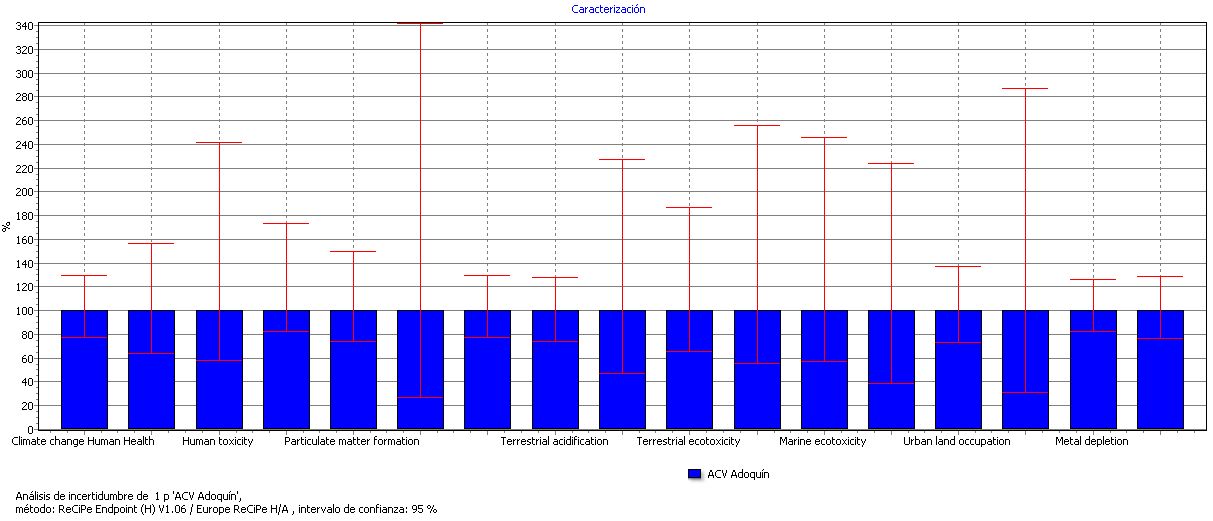
\includegraphics[width=15cm]{img/confianza_caracterizacion.png}
\caption[Intervalos de confianza para cada categoría de impacto a nivel de caracterización del ACV del adoquín.]{Intervalos de confianza para cada categoría de impacto a nivel de caracterización del ACV del adoquín. Fuente: elaboración propia.}
\label{fig:confianza_caracterizacion}
\end{figure}

Por cada categoría de impacto se indica un diagrama de barras con un margen de incertidumbre. El margen manifiesta el 95\% del intervalo de confiabilidad, lo que significa que el 95\% de los resultados estuvo dentro de este margen. Las figuras \ref{fig:confianza_caracterizacion},\ref{fig:confianza_normalizacion},\ref{fig:confianza_puntuacionunica} y \ref{fig:confianza_dano} muestran que los resultados del Análisis de Ciclo de Vida tienen una confianza del 95\%.

\begin{figure}[!htb]
\centering
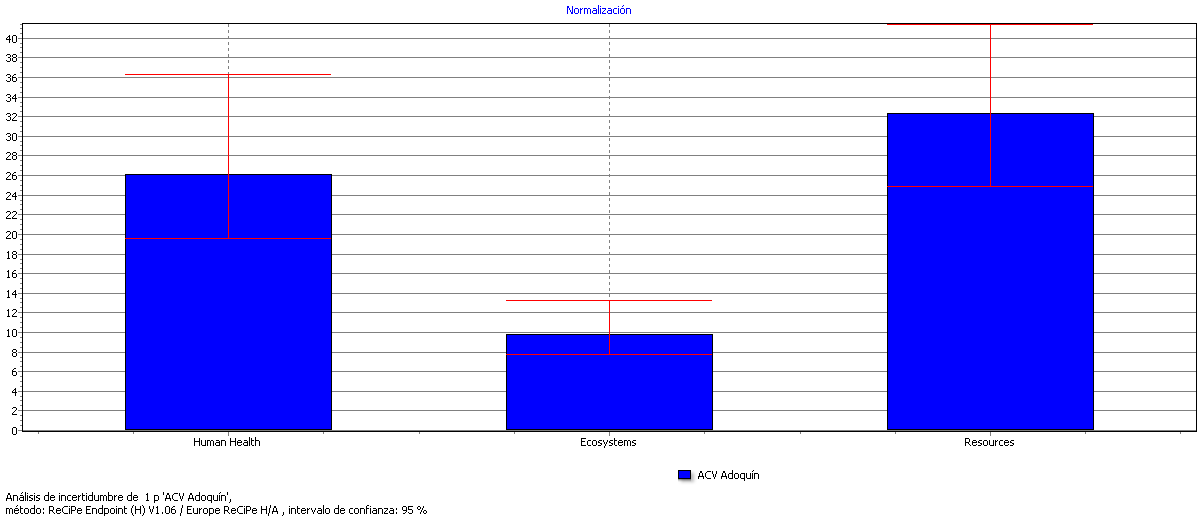
\includegraphics[width=15cm]{img/confianza_normalizacion.png}
\caption[Intervalos de confianza para cada categoría de impacto normalizada del ACV del adoquín.]{Intervalos de confianza para cada categoría de impacto normalizada del ACV del adoquín. Fuente: elaboración propia.}
\label{fig:confianza_normalizacion}
\end{figure}

\begin{figure}[!htb]
\centering
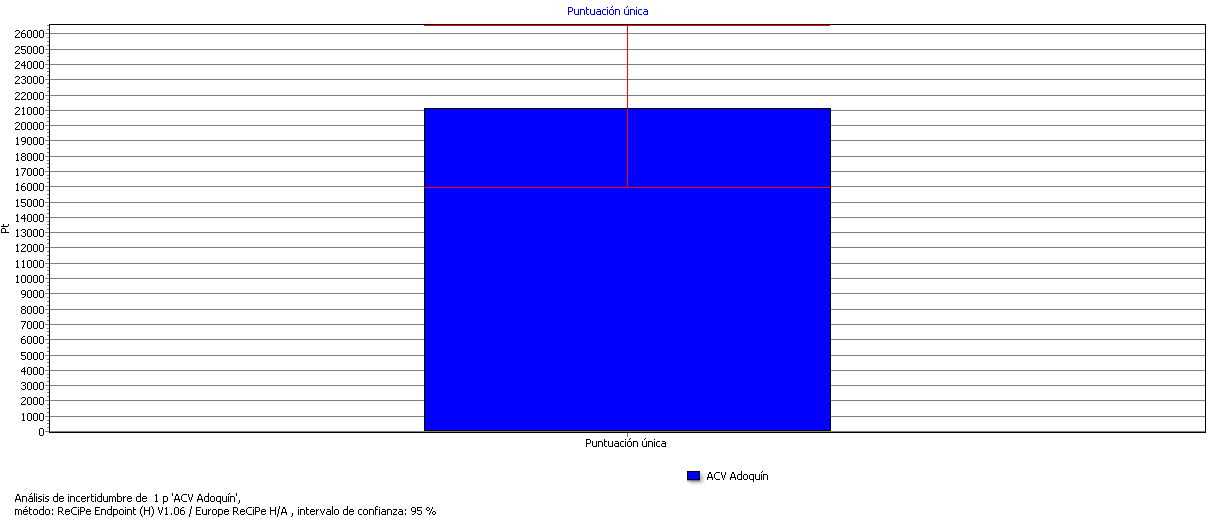
\includegraphics[width=15cm]{img/confianza_puntuacionunica.png}
\caption[Intervalos de confianza para cada categoría de impacto a nivel de puntuación única del ACV del adoquín.]{Intervalos de confianza para cada categoría de impacto a nivel de puntuación única del ACV del adoquín. Fuente: elaboración propia.}
\label{fig:confianza_puntuacionunica}
\end{figure}

\begin{figure}[!htb]
\centering
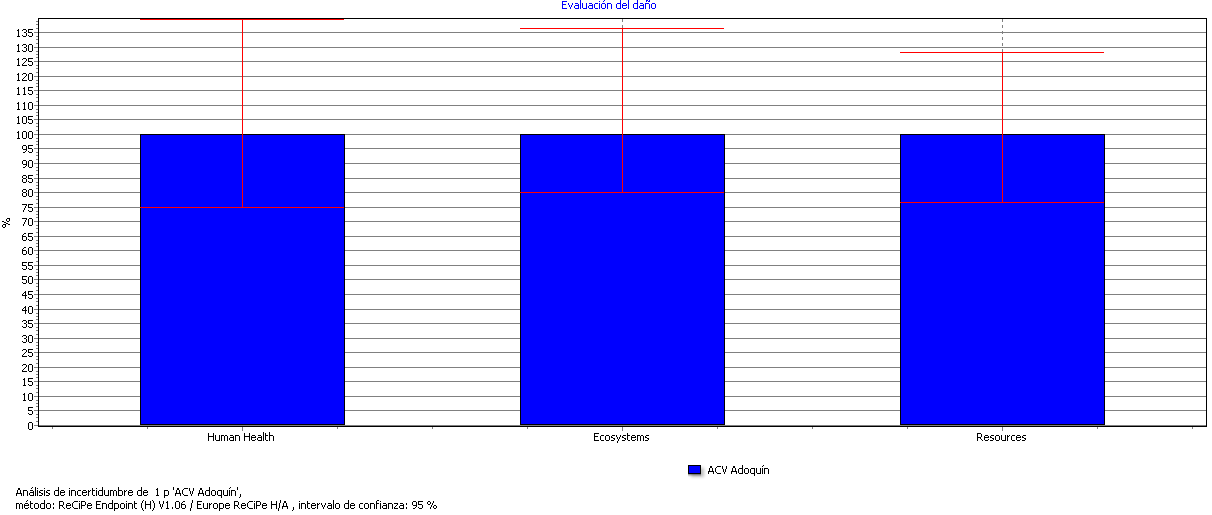
\includegraphics[width=15cm]{img/confianza_dano.png}
\caption[Intervalos de confianza para cada categoría de daño a nivel de puntuación única del ACV del adoquín.]{Intervalos de confianza para cada categoría de daño a nivel de puntuación única del ACV del adoquín. Fuente: elaboración propia.}
\label{fig:confianza_dano}
\end{figure}


\section{Verificación del análisis de coherencia}

La norma UNE-EN-ISO 14044:2006 indica que ``la verificación del análisis de coherencia busca determinar si las suposiciones, métodos, modelos y datos son coherentes a lo largo del ciclo de vida de un producto o entre distintas opciones''.

En este ACV no se realizan comparaciones entre diferentes opciones por lo que no hay comparaciones donde comprobar las incoherencias:
\begin{itemize}
  \item Fuente de datos: fabricante. Estado: OK.
  \item Exactitud de los datos: buena. Estado: OK
  \item Antigüedad de los datos: 2012—2013. Estado: OK
  \item Cobertura tecnológica: planta de fabricación. Estado: OK
  \item Cobertura relacionada con el tiempo: reciente . Estado: OK
  \item Cobertura geográfica: Málaga (España). Estado: OK
\end{itemize}

\section{Consideraciones}

El estudio del Análisis de Ciclo de Vida del adoquín indica que la etapa más influyente en el perfil medioambiental —usando el método ReCiPe—, la que mayor energía consume —con el método de Demanda de Energía Acumulada— y la que emite mayor cantidad de \ce{CO2} equivalente —por el método IPCC— es la de \textbf{extracción de materias primas, fabricación e instalación} (ver tabla \ref{perfil_medioambiental}).

\begin{table}[!htb]
\centering
\begin{tabular}{p{6cm}r}
\toprule
\multicolumn{2}{c}{Perfil medioambiental}\\
\midrule
\si{MJ} energía consumida & 1350\\
\si{kg} \ce{CO2} eq. & 58.1\\
\bottomrule
\end{tabular}
\caption[Perfil medioambiental de 1 \si{m^2} adoquín.]{Perfil medioambiental de 1 \si{m^2} adoquín. Fuente: elaboración propia.}
\label{perfil_medioambiental}
\end{table}

\subsection{Fase de extracción de materias primas, fabricación e instalación}
Para mejorar esta fase, habrá que centrarse en los tres procesos con mayor carga ambiental que se destacaron en la tabla \ref{categoriasimpactofabricacion}.

En primer lugar, la \textbf{capa bituminosa para base granular} se compone principalmente de dos procesos:
\begin{itemize}
  \item Obtención del material bituminoso: 99.73\%.
  \item Transporte: 0.27\%.
\end{itemize}

El problema principal de los materiales bituminosos es que su extracción y refinado son altamente complejos a nivel técnico y ambiental. La extracción suele realizarse mediante minería a cielo abierto, excavando la superficie y procesando la materia prima con calor y químicos in situ para decantar el betún y permitir que este fluya a través de oleoductos. El mayor inconveniente es que el 80\% de las arenas petrolíferas se encuentran a demasiada profundidad para poder extraerlas de esta forma lo que requiere operaciones aún más complejas bajo tierra \cite{eurobitume}.

Existen dos posibles alternativas para reducir el impacto ambiental. Se pueden utilizar pavimentos asfálticos reciclados añadidos directamente a la emulsión bituminosa como si fuese elemento más de la misma sustituyendo con ello a parte de ésta. Igualmente, puede emplearse también polvo de neumático de forma directa en la amasadora de la mezcla bituminosa como si se tratara de un árido mineral, pero al ser las partículas más finas, interaccionan con el betún modificando sus propiedades, consiguiendo mejorar el comportamiento de la mezcla bituminosa \cite{polvocaucho}.

Otra forma de poder mejorar este proceso es disminuir la distancia de transporte desde la planta de fabricación del material bituminoso hasta la zona de instalación del pavimento.

En segundo lugar, el \textbf{árido grueso para base granular} se compone de dos procesos:
\begin{itemize}
  \item Obtención de la arena caliza: 67.31\%.
  \item Transporte: 32.68\%
\end{itemize}

La base granular sobre la que van el resto de capas componentes del pavimento de adoquines es la más gruesa. Como alternativa al uso de arena caliza natural se puede recurrir principalmente al uso de áridos a partir de hormigón reciclado, que puede fragmentarse en diferentes tamaños según se requiera \cite{monografia}.

En este caso, la actuación sobre la distancia de recorrido del transporte del material supone algo más de un 30\% del total de la carga ambiental, por lo que acercando el lugar de extracción a la zona de instalación supondrá una mejora aceptable.

En tercer lugar, el \textbf{cemento Portland CEM I 52.5Z gris} se compone de dos procesos:
\begin{itemize}
  \item Obtención del cemento: 81.40\%.
  \item Transporte: 18.60\%
\end{itemize}

Actualmente existen nuevos productos que intentan reducir su impacto ambiental disminuyendo tanto la energía consumida en su producción como las emisiones de \ce{CO2} a la atmósfera. Por un lado, el CSIC-España (Centro Superior de Investigaciones Científicas) ha desarrollado un producto similar al cemento Portland aprovechando las cenizas volantes de la combustión del carbón\footnote{AAFA: Alkali-Activated Fly Ashes. Cenizas volantes de activación alcalina.} que necesita únicamente una temperatura de 60-80\si{\celsius} —frente a la temperatura habitual de 1450\si{\celsius}—, reduciendo las emisiones de \ce{CO2} un 50\% y un ahorro energético del 70\% \cite{csic}.

Por otro lado, se han creado nuevos tipos de cemento usando nanomateriales que permiten reducir hasta casi el 100\% de las emisiones directas de \ce{CO2} y en un 50\% la demanda energética en el proceso de síntesis del cemento mediante la sustitución de la piedra caliza por residuos sólidos de centrales térmicas \cite{website:tecnalia}.

También es posible sustituir el cemento convencional con cemento obtenido a partir de áridos reciclados procedentes de Residuos de Construcción y Demolición (RCD).

Respecto al transporte del cemento, la distancia de recorrido ya es bastante reducida —tan sólo 8 \si{km}— y supone un porcentaje relativamente bajo de mejora sobre el que actuar.

Por último, en referencia a todos los procesos de la etapa de extracción de materia prima, fabricación e instalación se puede actuar de forma indirecta modificando el mix eléctrico, disminuyendo la dependencia de las energías de origen fósil —que suponen un 88\% del total de la fase— y aumentando el uso de energías renovables. Debido a que las instalaciones disponen de una gran superficie, podría optarse por la instalación de paneles con células de tercera generación que permiten eficiencias de conversión eléctrica teóricas mayores que las anteriores.

Desde el punto de vista ambiental, el mayor impacto se produce en las categorías de \textbf{agotamiento de recursos fósiles} y \textbf{cambio climático}, debido principalmente a los tres procesos anteriormente mencionados. La \textbf{formación de partículas} y la \textbf{ocupación de tierras agrícolas} se deben también fundamentalmente a esta fase.

\subsection{Fase de uso y mantenimiento}
Respecto a la fase de \textbf{uso y mantenimiento}, el proceso de \textbf{sellado y vibrado del pavimento} es el objetivo a mejorar. El motivo principal es el uso de combustible fósil de tipo diesel para la alimentación de la máquina de planchas vibradoras. Se puede mejorar este proceso eligiendo una máquina con el menor consumo de combustible que ofrezca el mercado.

Desde el punto de vista ambiental, el mayor impacto se produce también en las categorías de \textbf{agotamiento de recursos fósiles} y \textbf{cambio climático}, debido principalmente a sellado y vibrado del pavimento.

\subsection{Fase de fin de vida}
La etapa de \textbf{fin de vida} produce un pequeño beneficio en comparación con la primera fase, que sirve como compensación de un 61\% de la carga ambiental de la segunda fase. Una mayor cercanía de las plantas de reciclaje disminuiría la distancia de transporte mejorando tanto las emisiones de \ce{CO2} como la energía empleada.

%!TEX root = informe.tex
\chapter{Conclusiones}\label{cap:conclusiones}
\section{Conclusiones generales}
En este proyecto se ha realizado un Análisis de Ciclo de Vida de un adoquín prefabricado de cemento de dimensiones 200\times 100\times 60 \si{mm}, tomando como unidad funcional un metro cuadrado del mismo.

El estudio de ACV supone una potente herramienta para detectar los procesos con mayor carga ambiental y los impactos ocasionados al medioambiente de forma normalizada y objetiva. Una vez se localizan estos puntos calientes pueden comunicarse a la empresa para realizar mejoras en el proceso repercutiendo bien energéticamente, económicamente o como publicidad de tipo ambiental. Se puede recurrir al etiquetado ambiental \cite{iso14020} para estimular la demanda de productos y servicios con menores cargas ambientales indicando información relevante sobre su ciclo de vida —tal como la energía consumida o la cantidad de \ce{CO2} generado— y así satisfacer una demanda creciente de productos con información ambiental.

La carga ambiental mayor se produce en la fase del ciclo de vida de extracción de materias primas, fabricación e instalación, siendo la fase de uso y mantenimiento muy inferior aunque no despreciable y la de fin de vida tomada en consideración por los beneficios ambientales que aporta.

Los procesos unitarios donde se producen las mayores cargas ambientales son la extracción de materias primas para la capa bituminosa y el árido grueso de la capa base de la instalación y el proceso de fabricación del cemento Portland.

La fase del Análisis de Ciclo de Vida más compleja es la de Inventario de Ciclo de Vida, debido a que el inventario que ofrece la base de datos \textit{ecoinvent} no disponía de la amplia mayoria de procesos que intervienen en este proyecto y la información disponible era muy reducida. También ha aportado complejidad a la realización de este proyecto la baja disponibilidad de otros proyectos que sirvieran de base que utilizaran el ACV como método de estudio en este sector.

El software de análisis SimaPro ha simplificado en gran medida la fase de Evaluación del Inventario de Ciclo de Vida y la de Interpretación, no sólo por la incorporación del método ReCiPe, sino por su adaptación del flujo de trabajo a la normativa UNE-EN-ISO 14040:2006 y 14044:2006.


\section{Futuros trabajos y ampliaciones}

Este método de análisis desarrollado durante este proyecto es aplicable no sólo a adoquines sino a cualquier producto o servicio, por lo que se puede usar como base para otros productos prefabricados del cemento u otros tipos de pavimentos como el de asfalto o cerámico para poder hacer comparaciones entre ellos.

También se podría ampliar el estudio a otros países —donde cambiaría el mix eléctrico— u otros procesos alternativos de fabricación distintos al de este estudio.

\cleardoublepage

\part{Anexos}
\parttoc
\begin{appendices}
%!TEX root = informe.tex
\chapter{Datos proporcionados por el fabricante}\label{apend:datos}
En este apéndice se incluyen los datos proporcionados por el fabricante acerca del proceso de producción.

\begin{table}[!htb]
\centering
\begin{tabular}{lccc}
\toprule
\multicolumn{4}{c}{Fórmula base para de adoquín Holanda 6}\\
\midrule
Materia prima & \% Fórmula & Proced. & Dist. (\si{km})\\
\midrule
Árido tipo 5/7 & 37.75 & Alh. Torre & 8\\
Arena tipo 0/5 & 47.16 & Alh. Torre & 8\\
Cemento Portland 52.5N & 10.06 & Málaga-El Palo & 30\\
Agua & 5.03 & Red & -\\
\bottomrule
\end{tabular}
\caption{Fórmula base para de adoquín Holanda 6.}
\label{formulabase}
\end{table}

\begin{figure}[!htb]
\centering
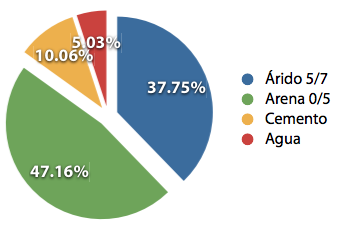
\includegraphics[width=6cm]{porcent_matprima.png}
\caption{Porcentajes de materías prima para adoquín.}
\label{fig:porcentmatprima}
\end{figure}

\begin{table}[!htp]
\centering
\begin{tabular}{lcrrr}
\toprule
\multicolumn{5}{c}{Tiempo de proceso y energía por \si{m^2} de adoquín fabricado}\\
\midrule
Proceso & Duración (\si{s}) & Pot. (\si{kW}) & Energía (\si{kJ}) & Energía (\si{MJ})\\
\midrule
Dosif. arena & 3 & 0.7 & 2.1 & 0.0021\\
Dosif. áridos & 3 & 0.7 & 2.1 & 0.0021\\
Cinta transp. arena y áridos  & 21 & 8.7 & 182.7 & 0.1827\\
Cinta transp. cemento & 15 & 6.5 & 97.5 & 0.0975\\
Skip  & 27 & 15 & 405 & 0.405\\
Mezcladora & 42 & 31 & 1302 & 1.302\\
Cinta transp. hormigón & 11 & 8 & 88 & 0.088\\
Tolva hormigón 1/2 & 23 & 0.7 & 16.1 & 0.0161\\
Prensado 1/2 & 19 & 23 & 437 & 0.437\\
Cinta transp. piezas frescas 1/2 & 14 & 5.5 & 77 & 0.077\\
Ascensor 1/2 & 1 & 7 & 7 & 0.007\\
Tolva hormigón 2/2 & 23 & 0.7 & 16.1 & 0.0161\\
Prensado 2/2 & 19 & 23 & 437 & 0.437\\
Cinta piezas frescas 2/2 & 14 & 5.5 & 77 & 0.077\\
Ascensor 2/2 & 17 & 7 & 119 & 0.119\\
Multiforca ida & 43 & 12 & 516 & 0.516\\
Multiforca vuelta & 43 & 12 & 516 & 0.516\\
Descensor 1/2 & 17 & 7 & 119 & 0.119\\
Descensor 2/2 & 1 & 7 & 7 & 0.007\\
Transp. bandejas hasta paletiz. & 14 & 1.5 & 21 & 0.021\\
Paletizadora & 10 & 5 & 50 & 0.05\\
Transp. palet & 14 & 1.7 & 23.8 & 0.0238\\
Flejadora & 10 & 1.5 & 15 & 0.015\\
Transp. rodillos hasta recogida  & 21 & 1.5 & 31.5 & 0.0315\\
Control informatizado & 405 & 1.2 & 486 & 0.486\\
Iluminación & 405 & 2.4 & 972 & 0.972\\
\bottomrule
\end{tabular}
\caption{Desglose de procesos y energías del fabricante por \si{m^2} de adoquín fabricado.}
\label{desgloseenergia}
\end{table}

\begin{figure}[!htb]
\centering
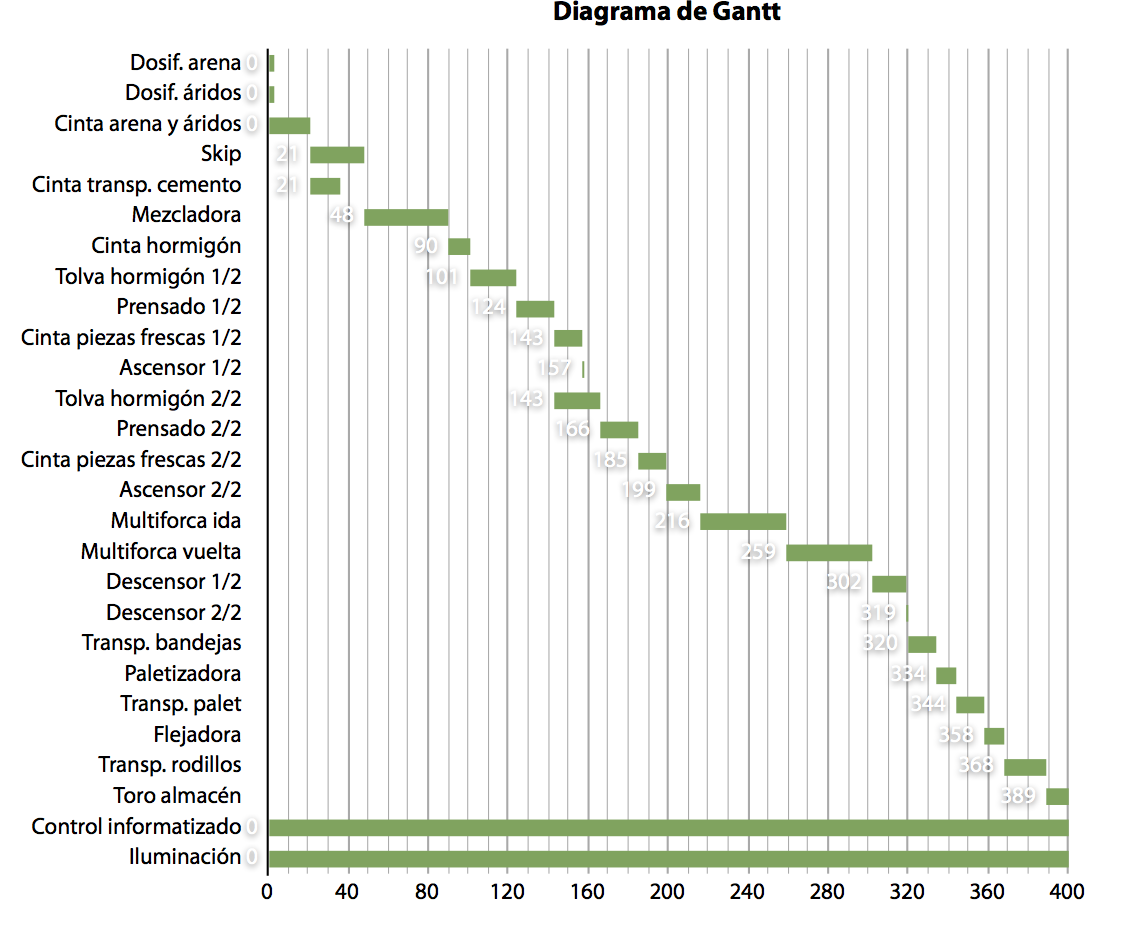
\includegraphics[width=15cm]{gantt.png}
\caption{Diagrama de Gantt de los procesos de fabricación.}
\label{fig:gant}
\end{figure}

\cleardoublepage
% %!TEX root = informe.tex
\chapter{Resultados de SimaPro}\label{apend:simapro}
En este apéndice se incluyen los resultados de la aplicación de software SimaPro.

% \cleardoublepage
%!TEX root = informe.tex
\chapter{Catálogo Adoquín Holanda 6}\label{apend:catalogo}
En este apéndice se incluyen los planos de la planta de fabricación de materiales prefabricados y los modelos de fabricación del adoquín y su molde.

\newpage
\begin{figure}[!htb]
\centering
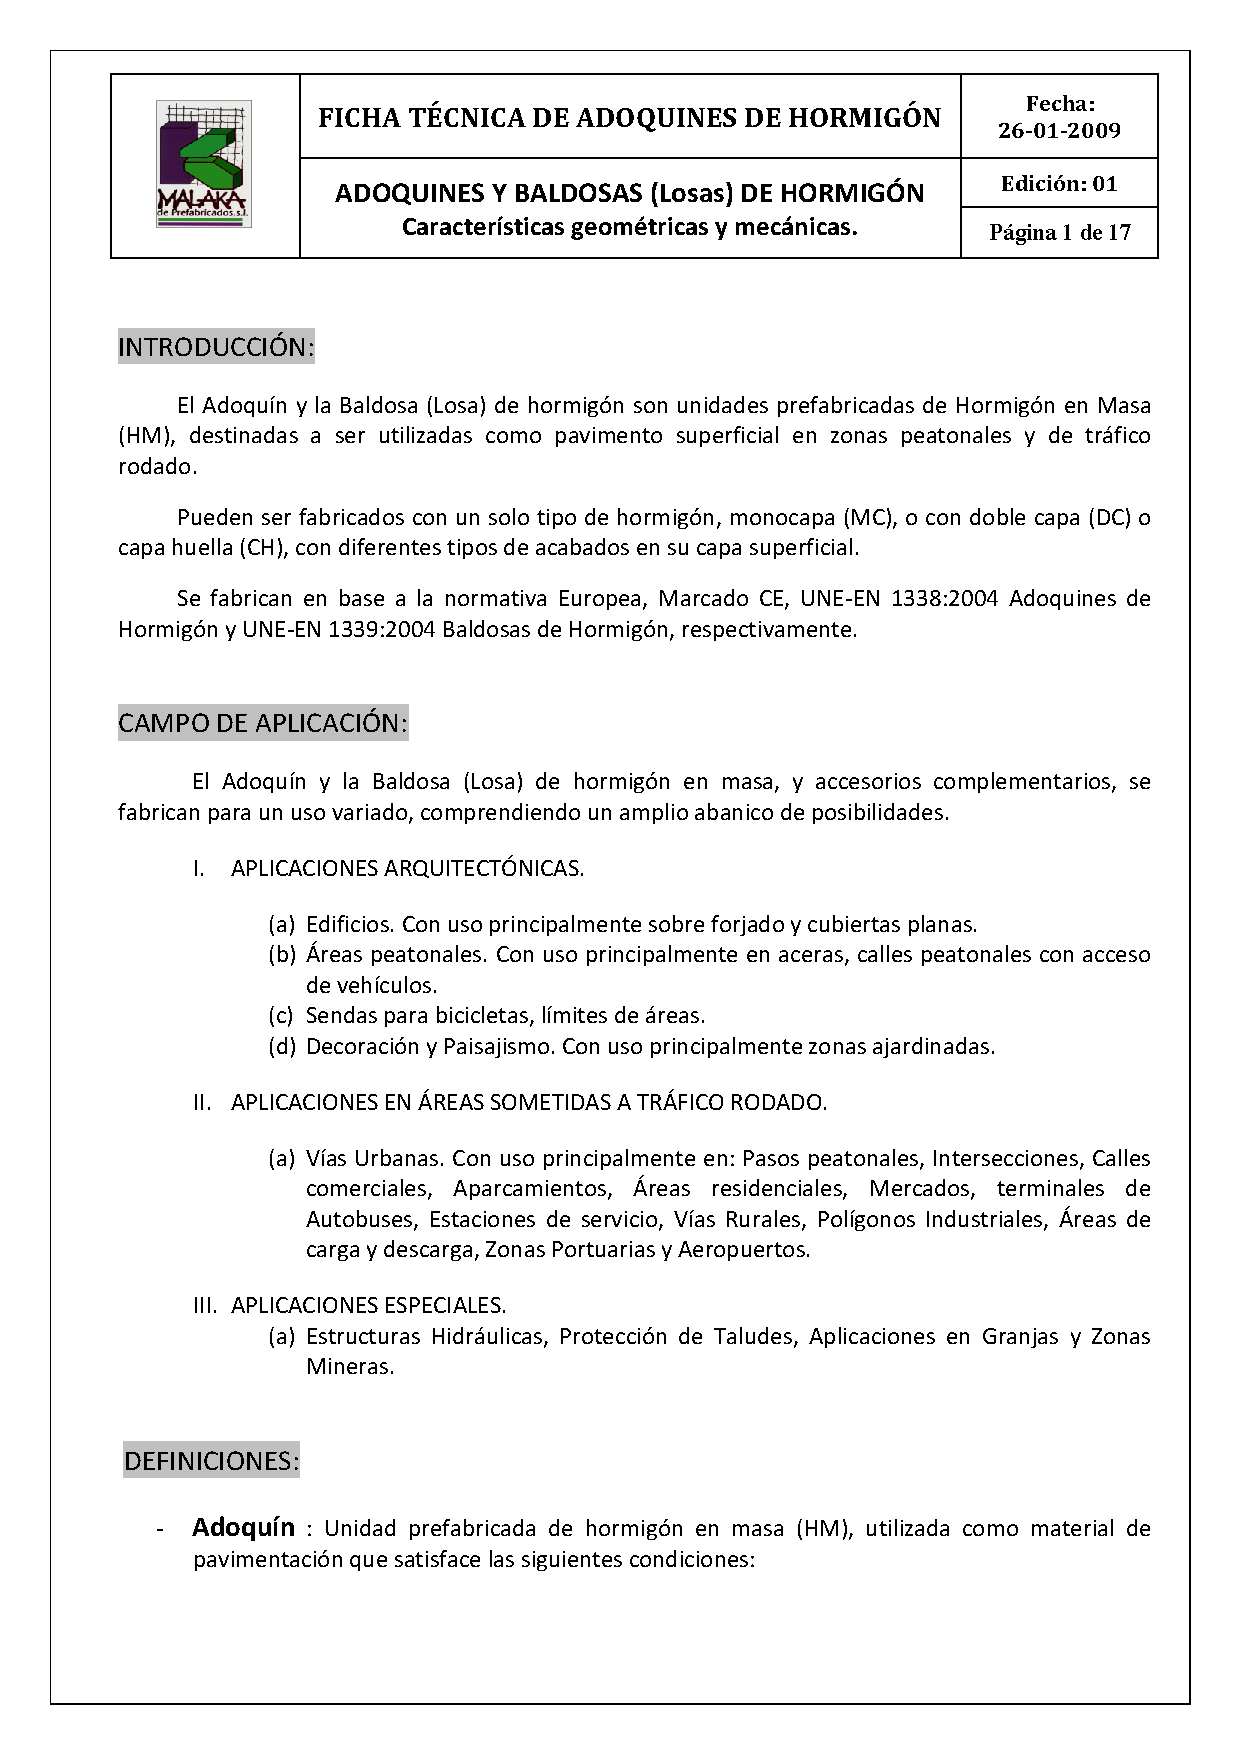
\includegraphics[scale=0.68]{ficha_tecnica/ft_adoquin_1.pdf}
\label{fig:ftadoquin1}
\end{figure}
\newpage
\begin{figure}[!htb]
\centering
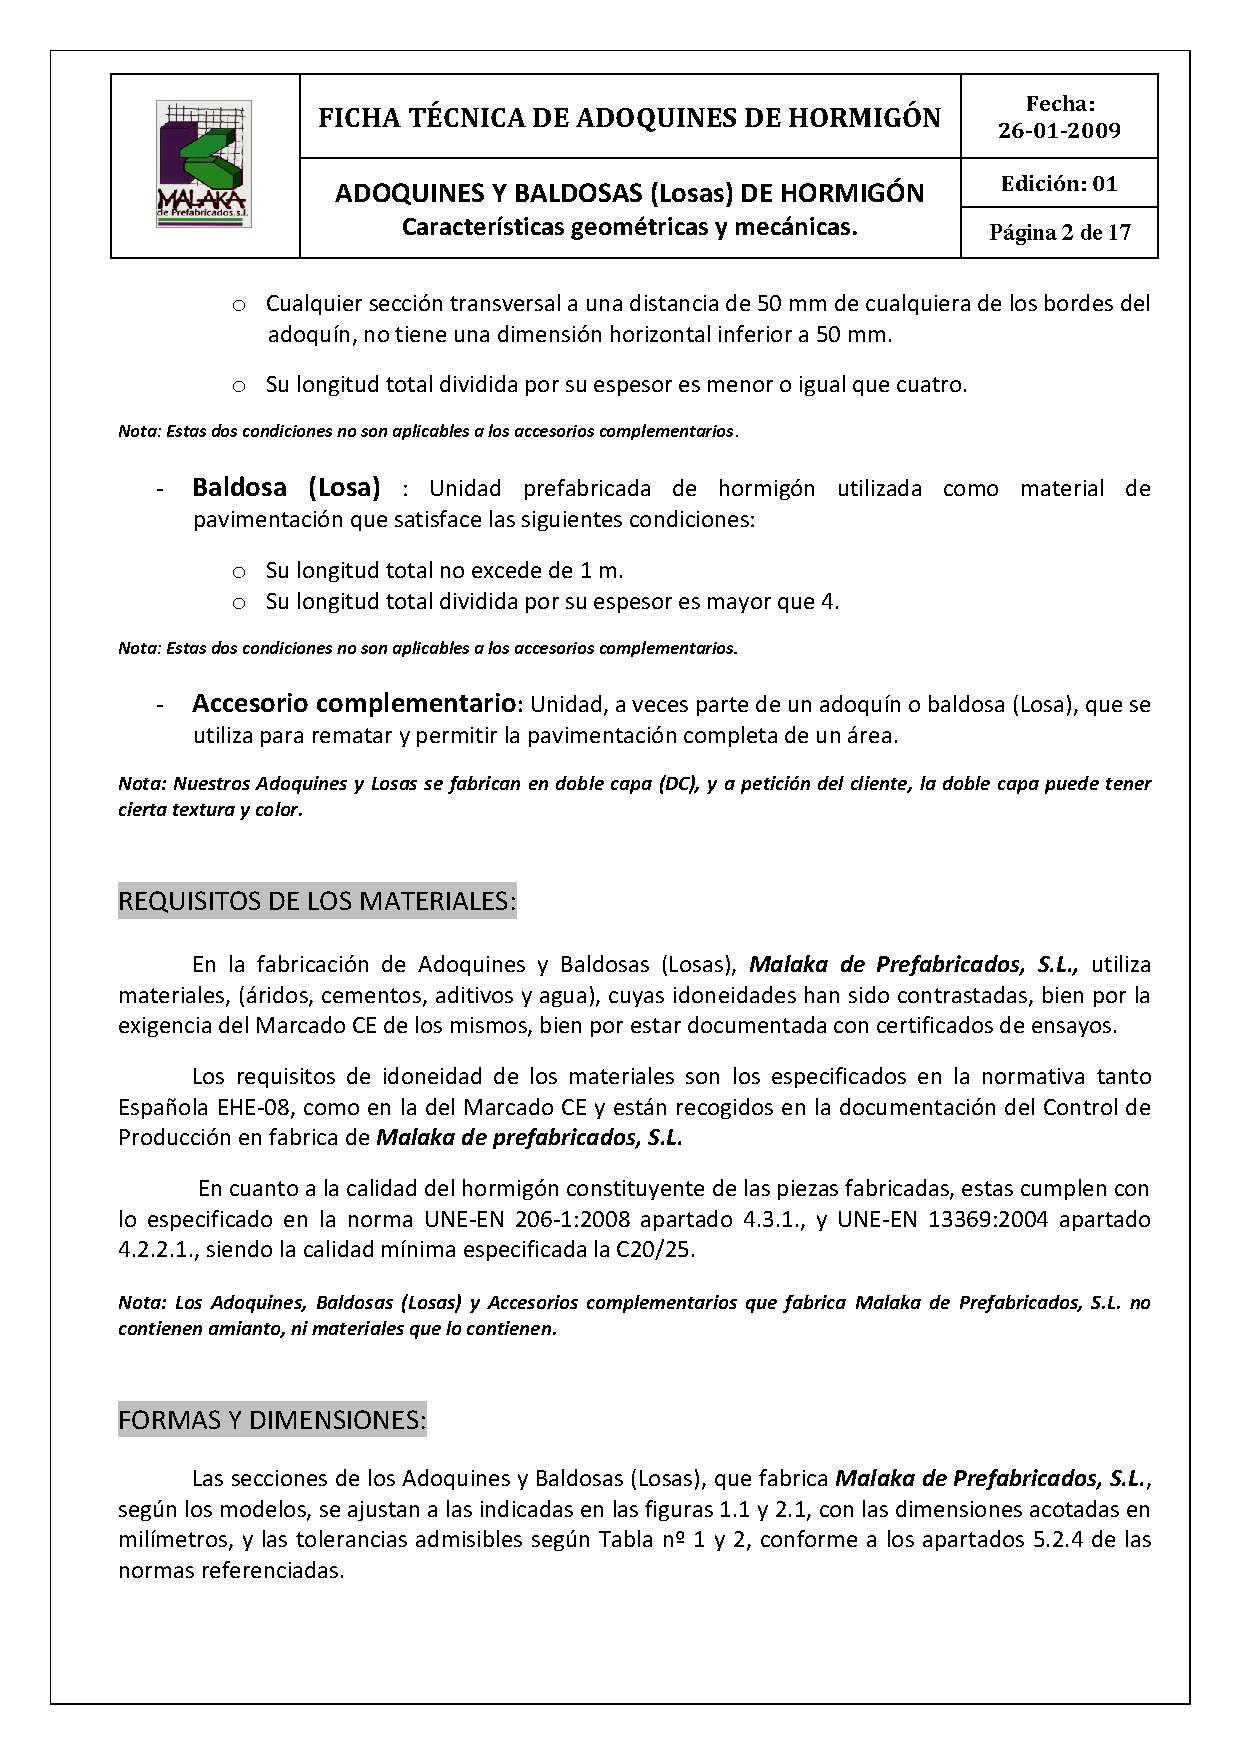
\includegraphics[scale=0.68]{ficha_tecnica/ft_adoquin_2.pdf}
\label{fig:ftadoquin2}
\end{figure}
\newpage
\begin{figure}[!htb]
\centering
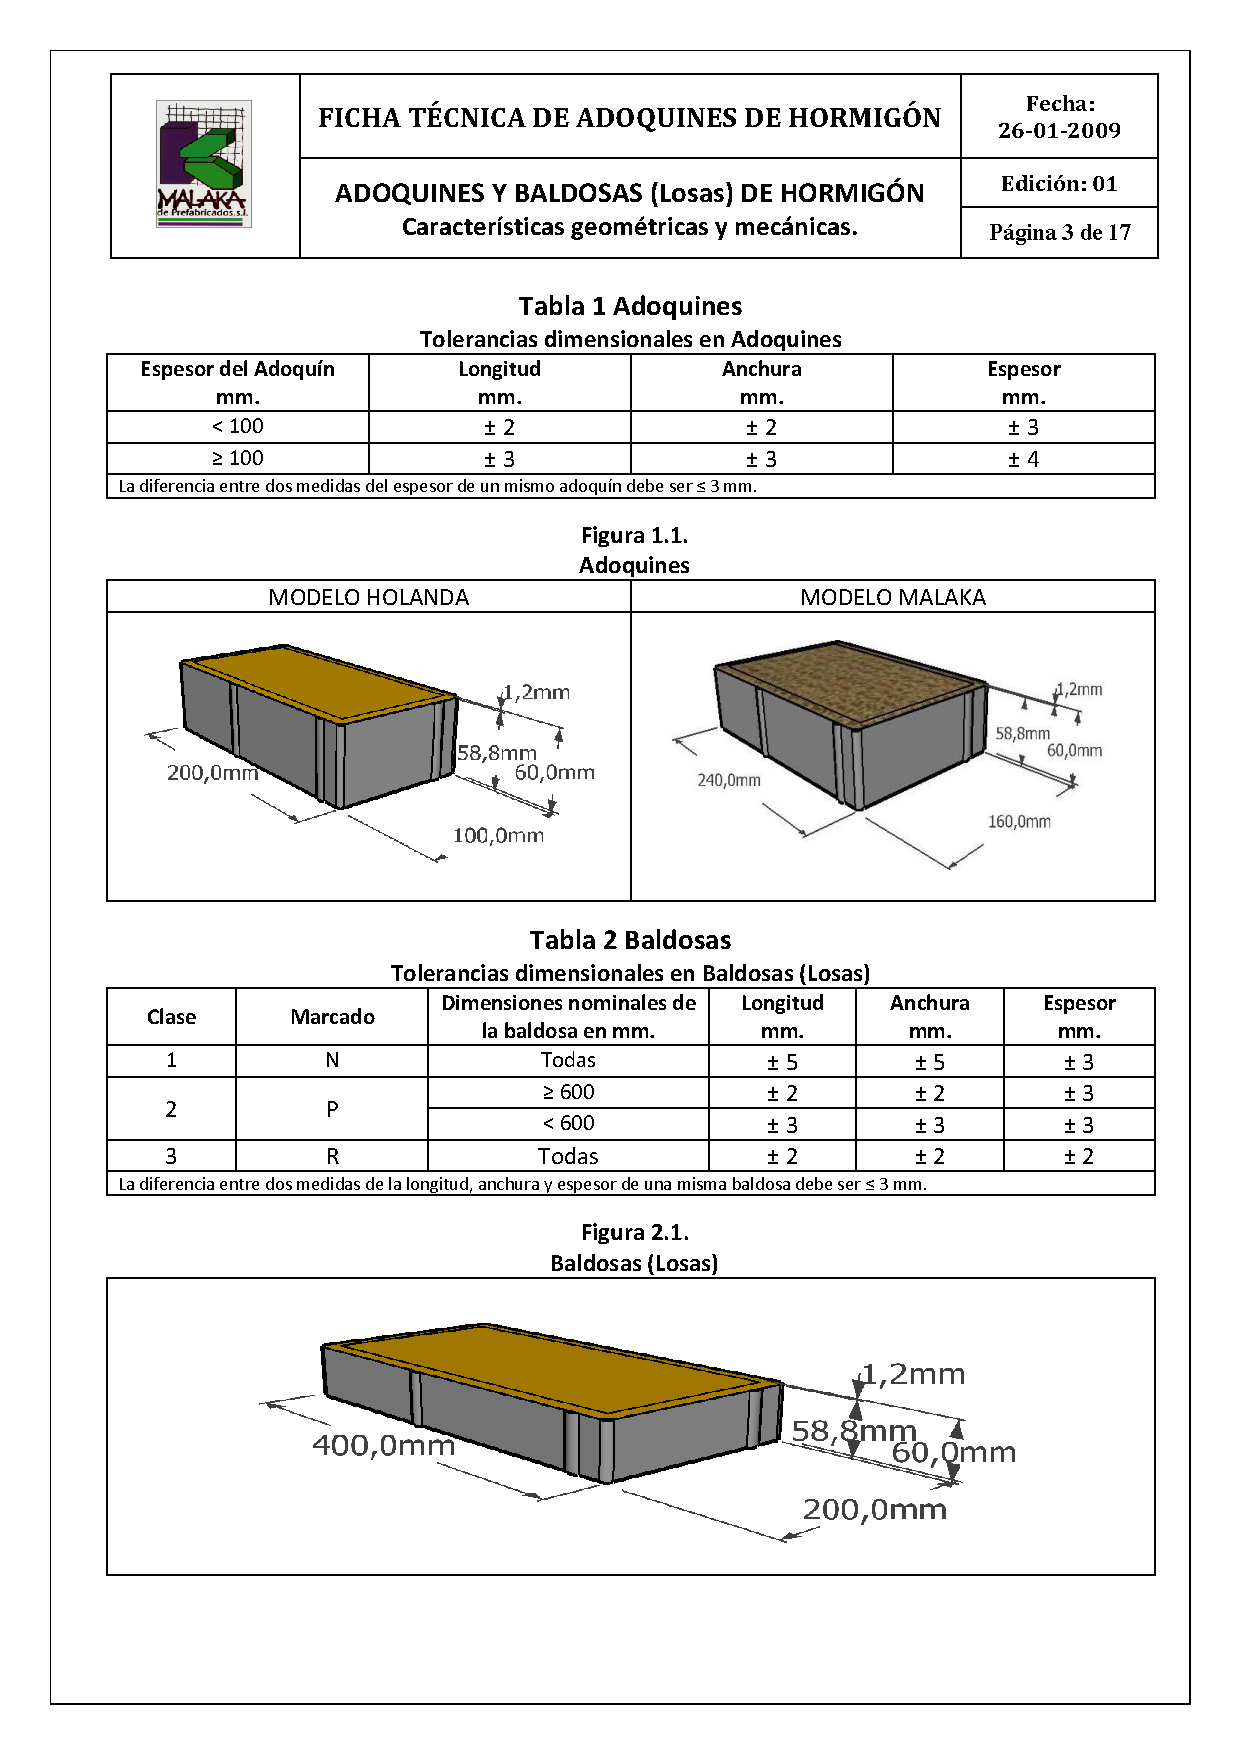
\includegraphics[scale=0.68]{ficha_tecnica/ft_adoquin_3.pdf}
\label{fig:ftadoquin3}
\end{figure}
\newpage
\begin{figure}[!htb]
\centering
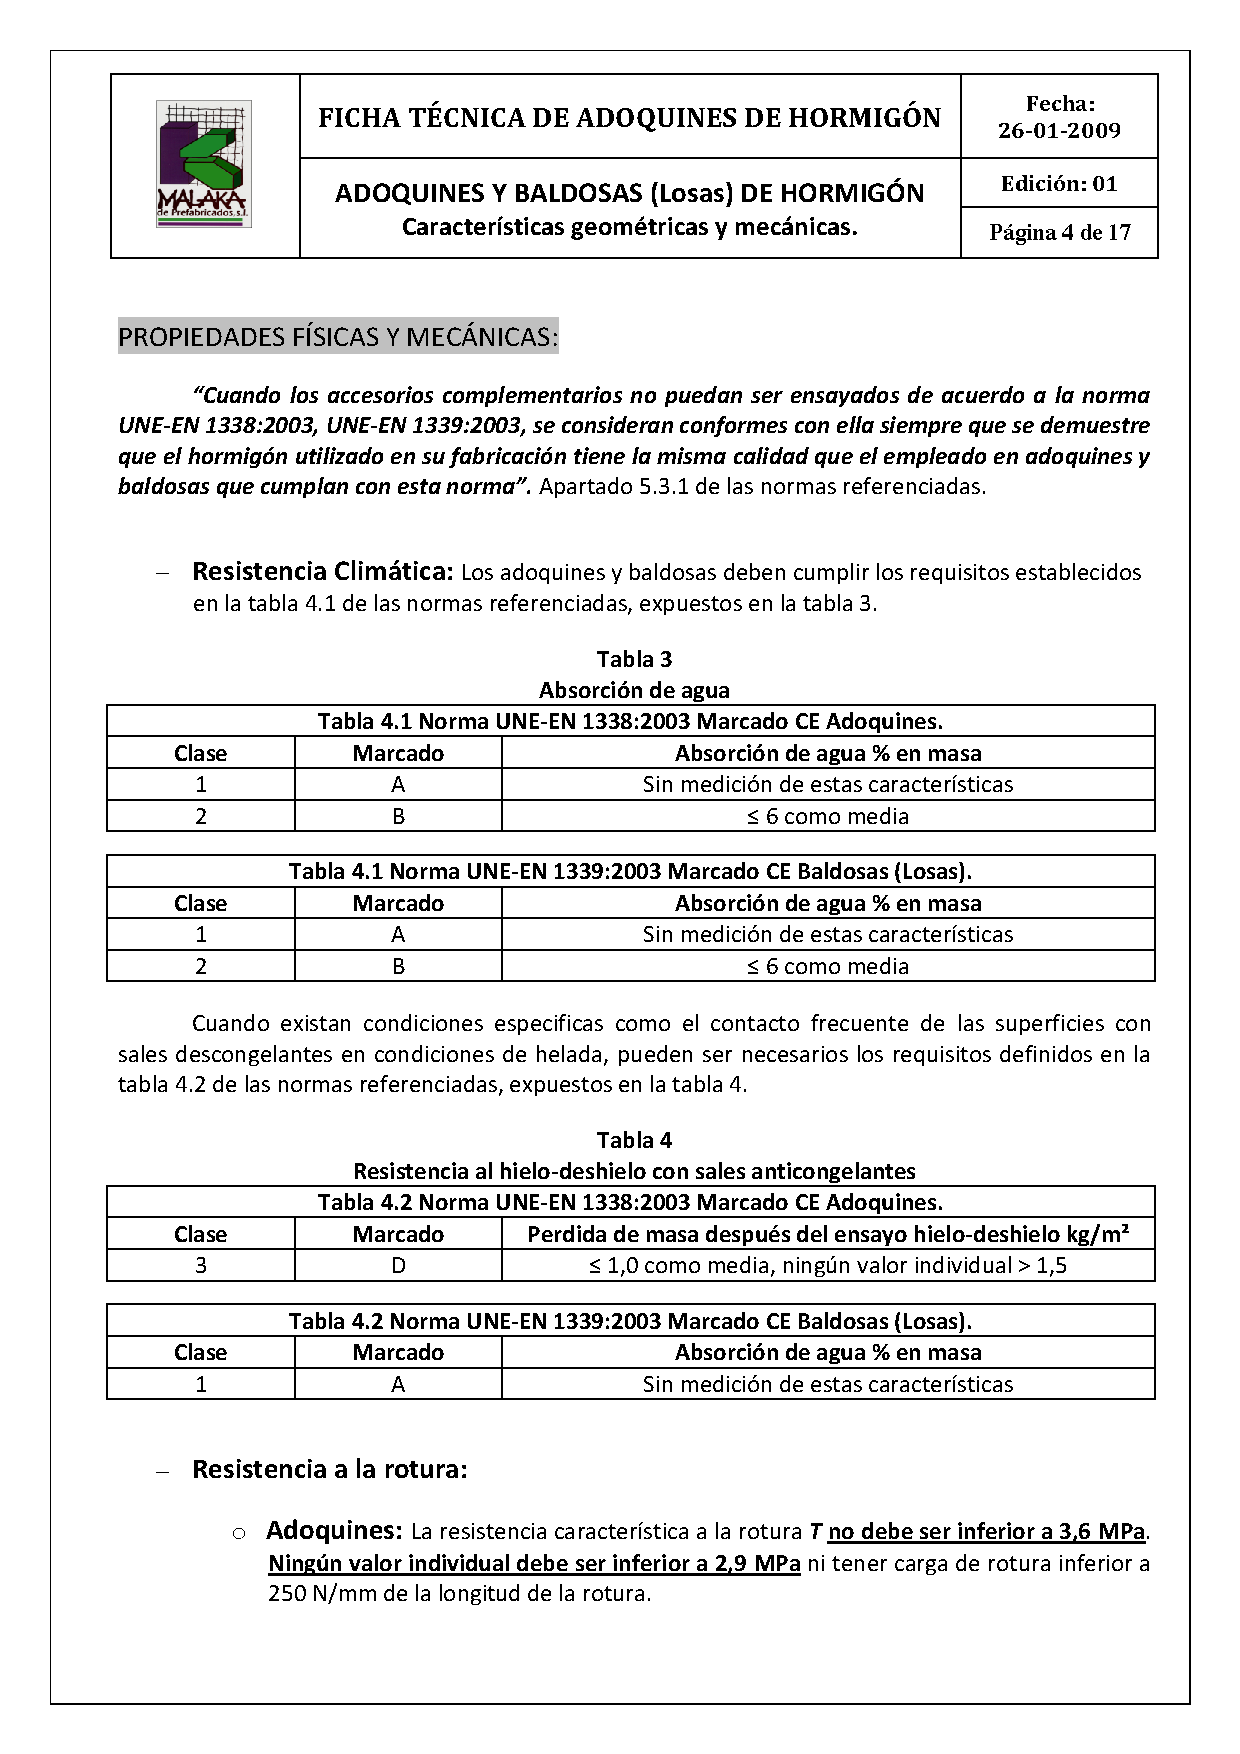
\includegraphics[scale=0.68]{ficha_tecnica/ft_adoquin_4.pdf}
\label{fig:ftadoquin4}
\end{figure}
\newpage
\begin{figure}[!htb]
\centering
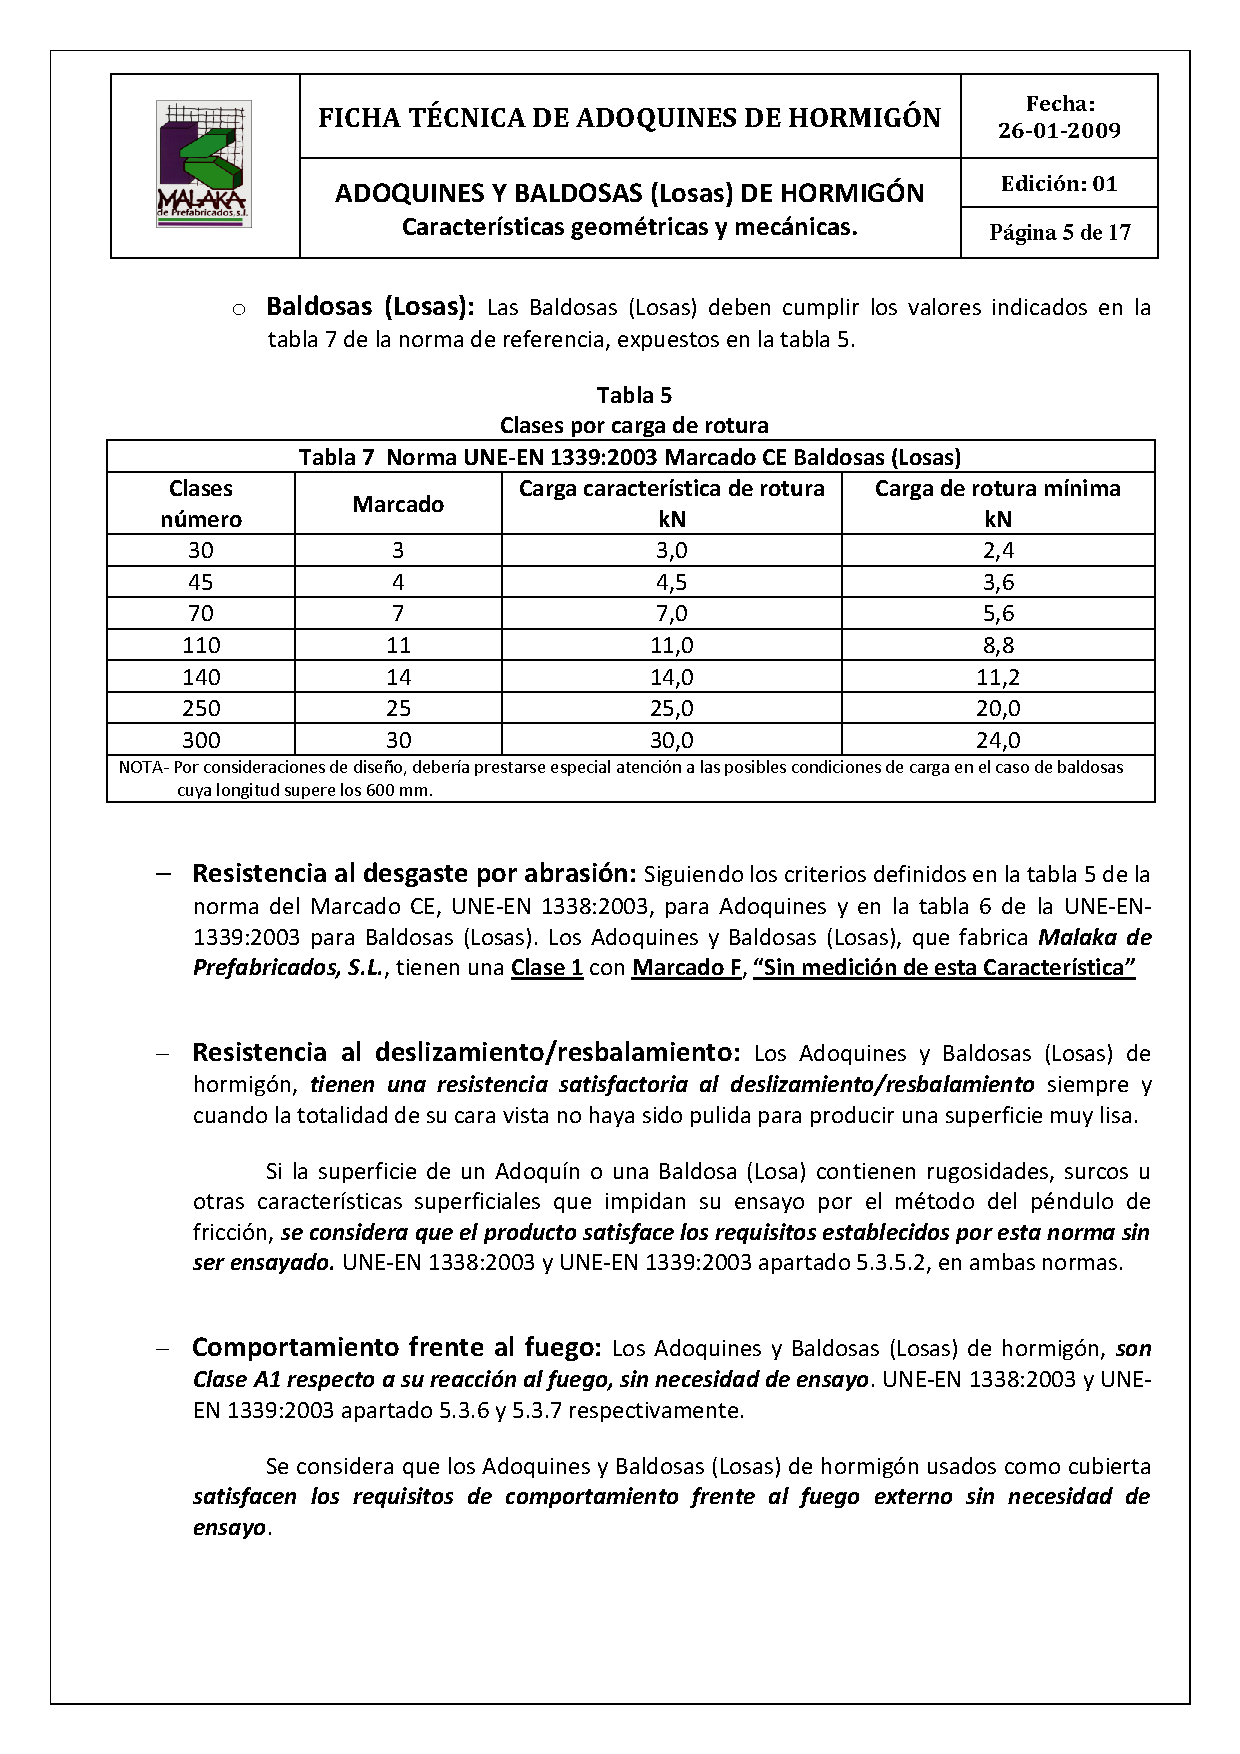
\includegraphics[scale=0.68]{ficha_tecnica/ft_adoquin_5.pdf}
\label{fig:ftadoquin5}
\end{figure}
\newpage
\begin{figure}[!htb]
\centering
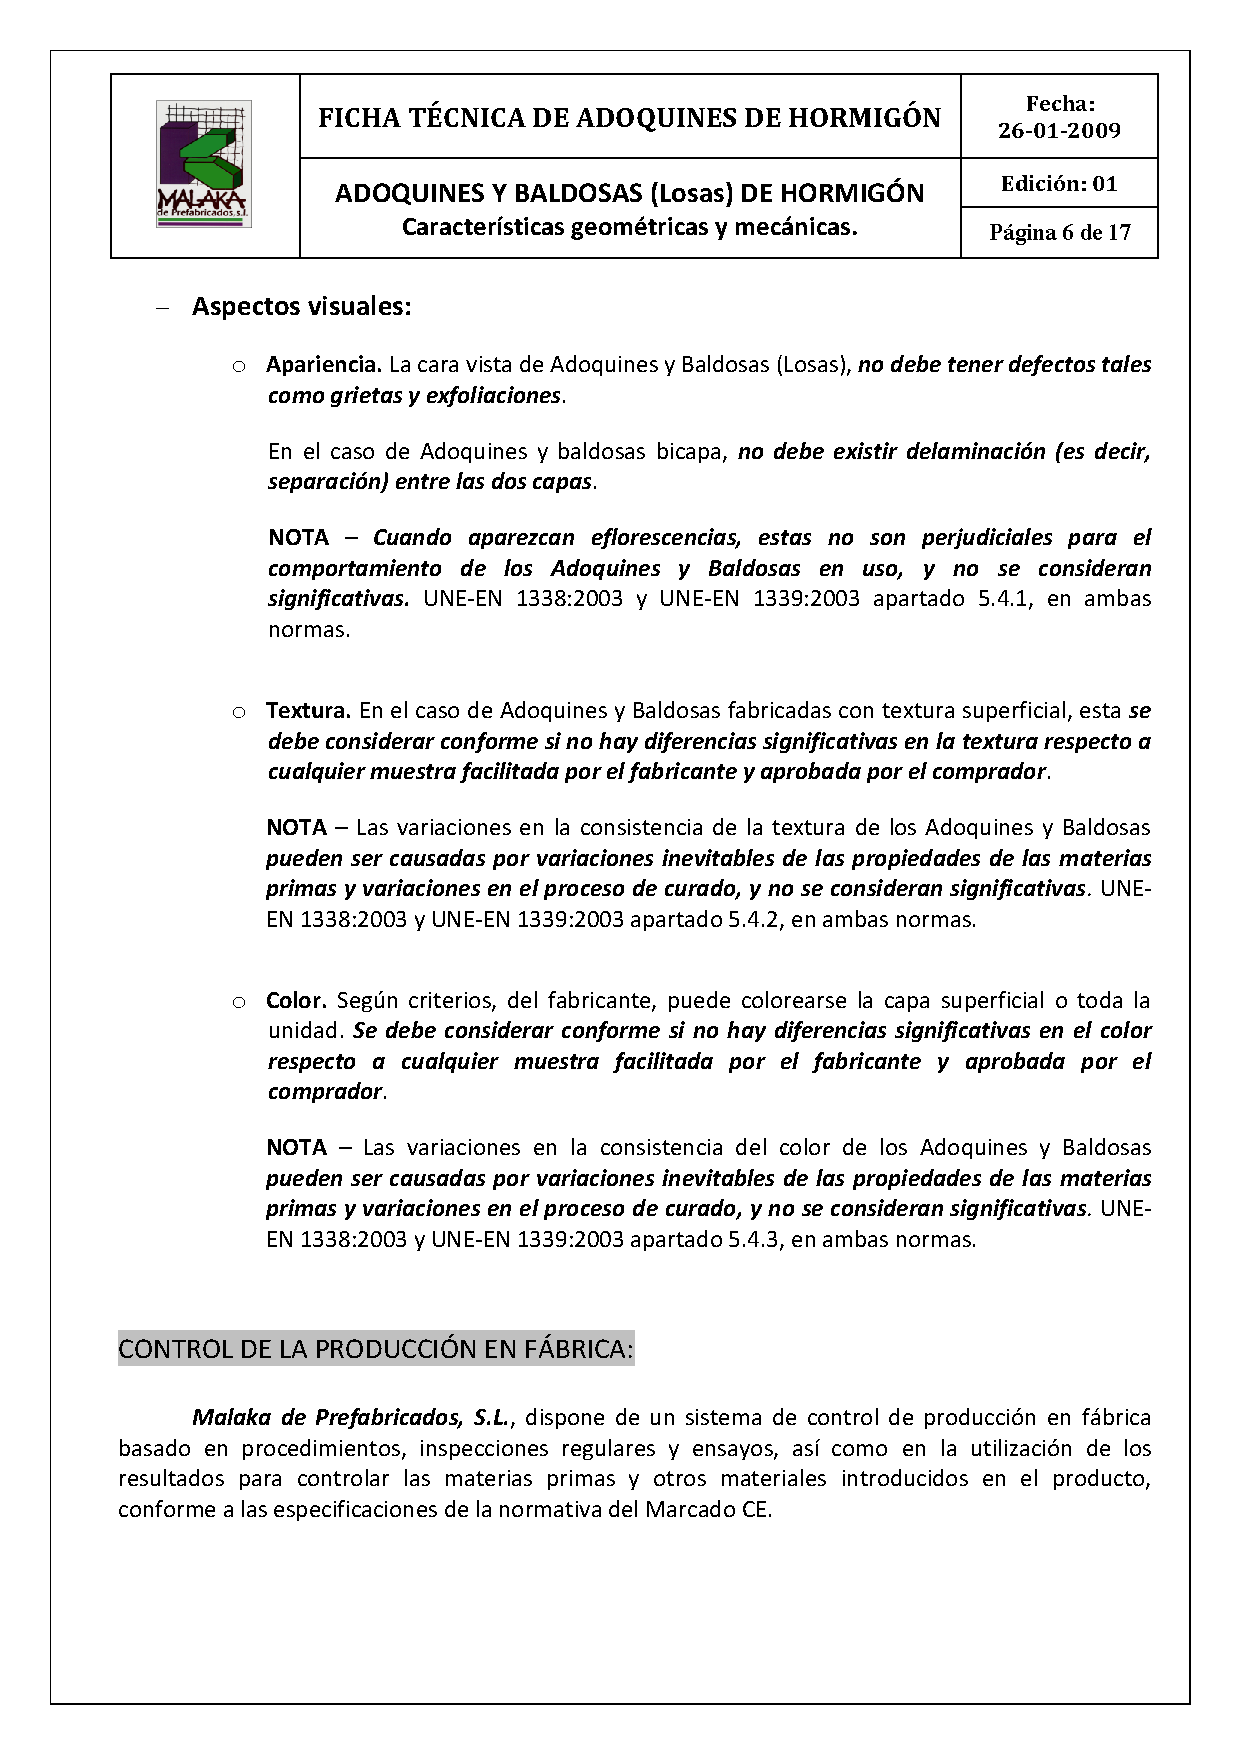
\includegraphics[scale=0.68]{ficha_tecnica/ft_adoquin_6.pdf}
\label{fig:ftadoquin6}
\end{figure}

\cleardoublepage
%!TEX root = informe.tex
\chapter{Herramientas utilizadas}\label{apend:herramientas}

Este proyecto ha sido tipografiado con el sistema de composición de documentos Xe\LaTeX. \LaTeX\ y Xe\LaTeX\ son distribuidos con el Mac\TeX, una redistribución de \TeX\ Live para OS X. La bibliografía ha sido generada mediante el sistema de gestión de referencias Bib\TeX.

Para la redacción se ha utilizado el editor de texto Sublime Text con el paquete LaTeXTools para la automatización de macros. Las fuentes de impresión empleadas son Minion Pro y Myriad Pro de Adobe.

Se ha utilizado un ordenador Apple Macbook Pro con sistema operativo OS X.

La generación de diagramas se ha realizado con MindNode para Mac y los paquetes de programación TikZ y PGF para Xe\LaTeX.

El software de Análisis de Ciclo de Vida elegido es SimaPro de PRé Consultants.

Los planos han sido creados usando el programa AutoCAD de Autodesk.

Las copias de seguridad se han realizado con el software de control de versiones Git en un repositorio online de Github y soporte local con Time Machine de Apple.

\cleardoublepage
\end{appendices}

\part{Planos}\label{planos}
\parttoc
%!TEX root = informe.tex
\setcounter{chapter}{1}
\addcontentsline{toc}{chapter}{\protect\numberline{\thechapter}Plano modelo adoquín Holanda 6}

\begin{figure}[!htb]
\centering
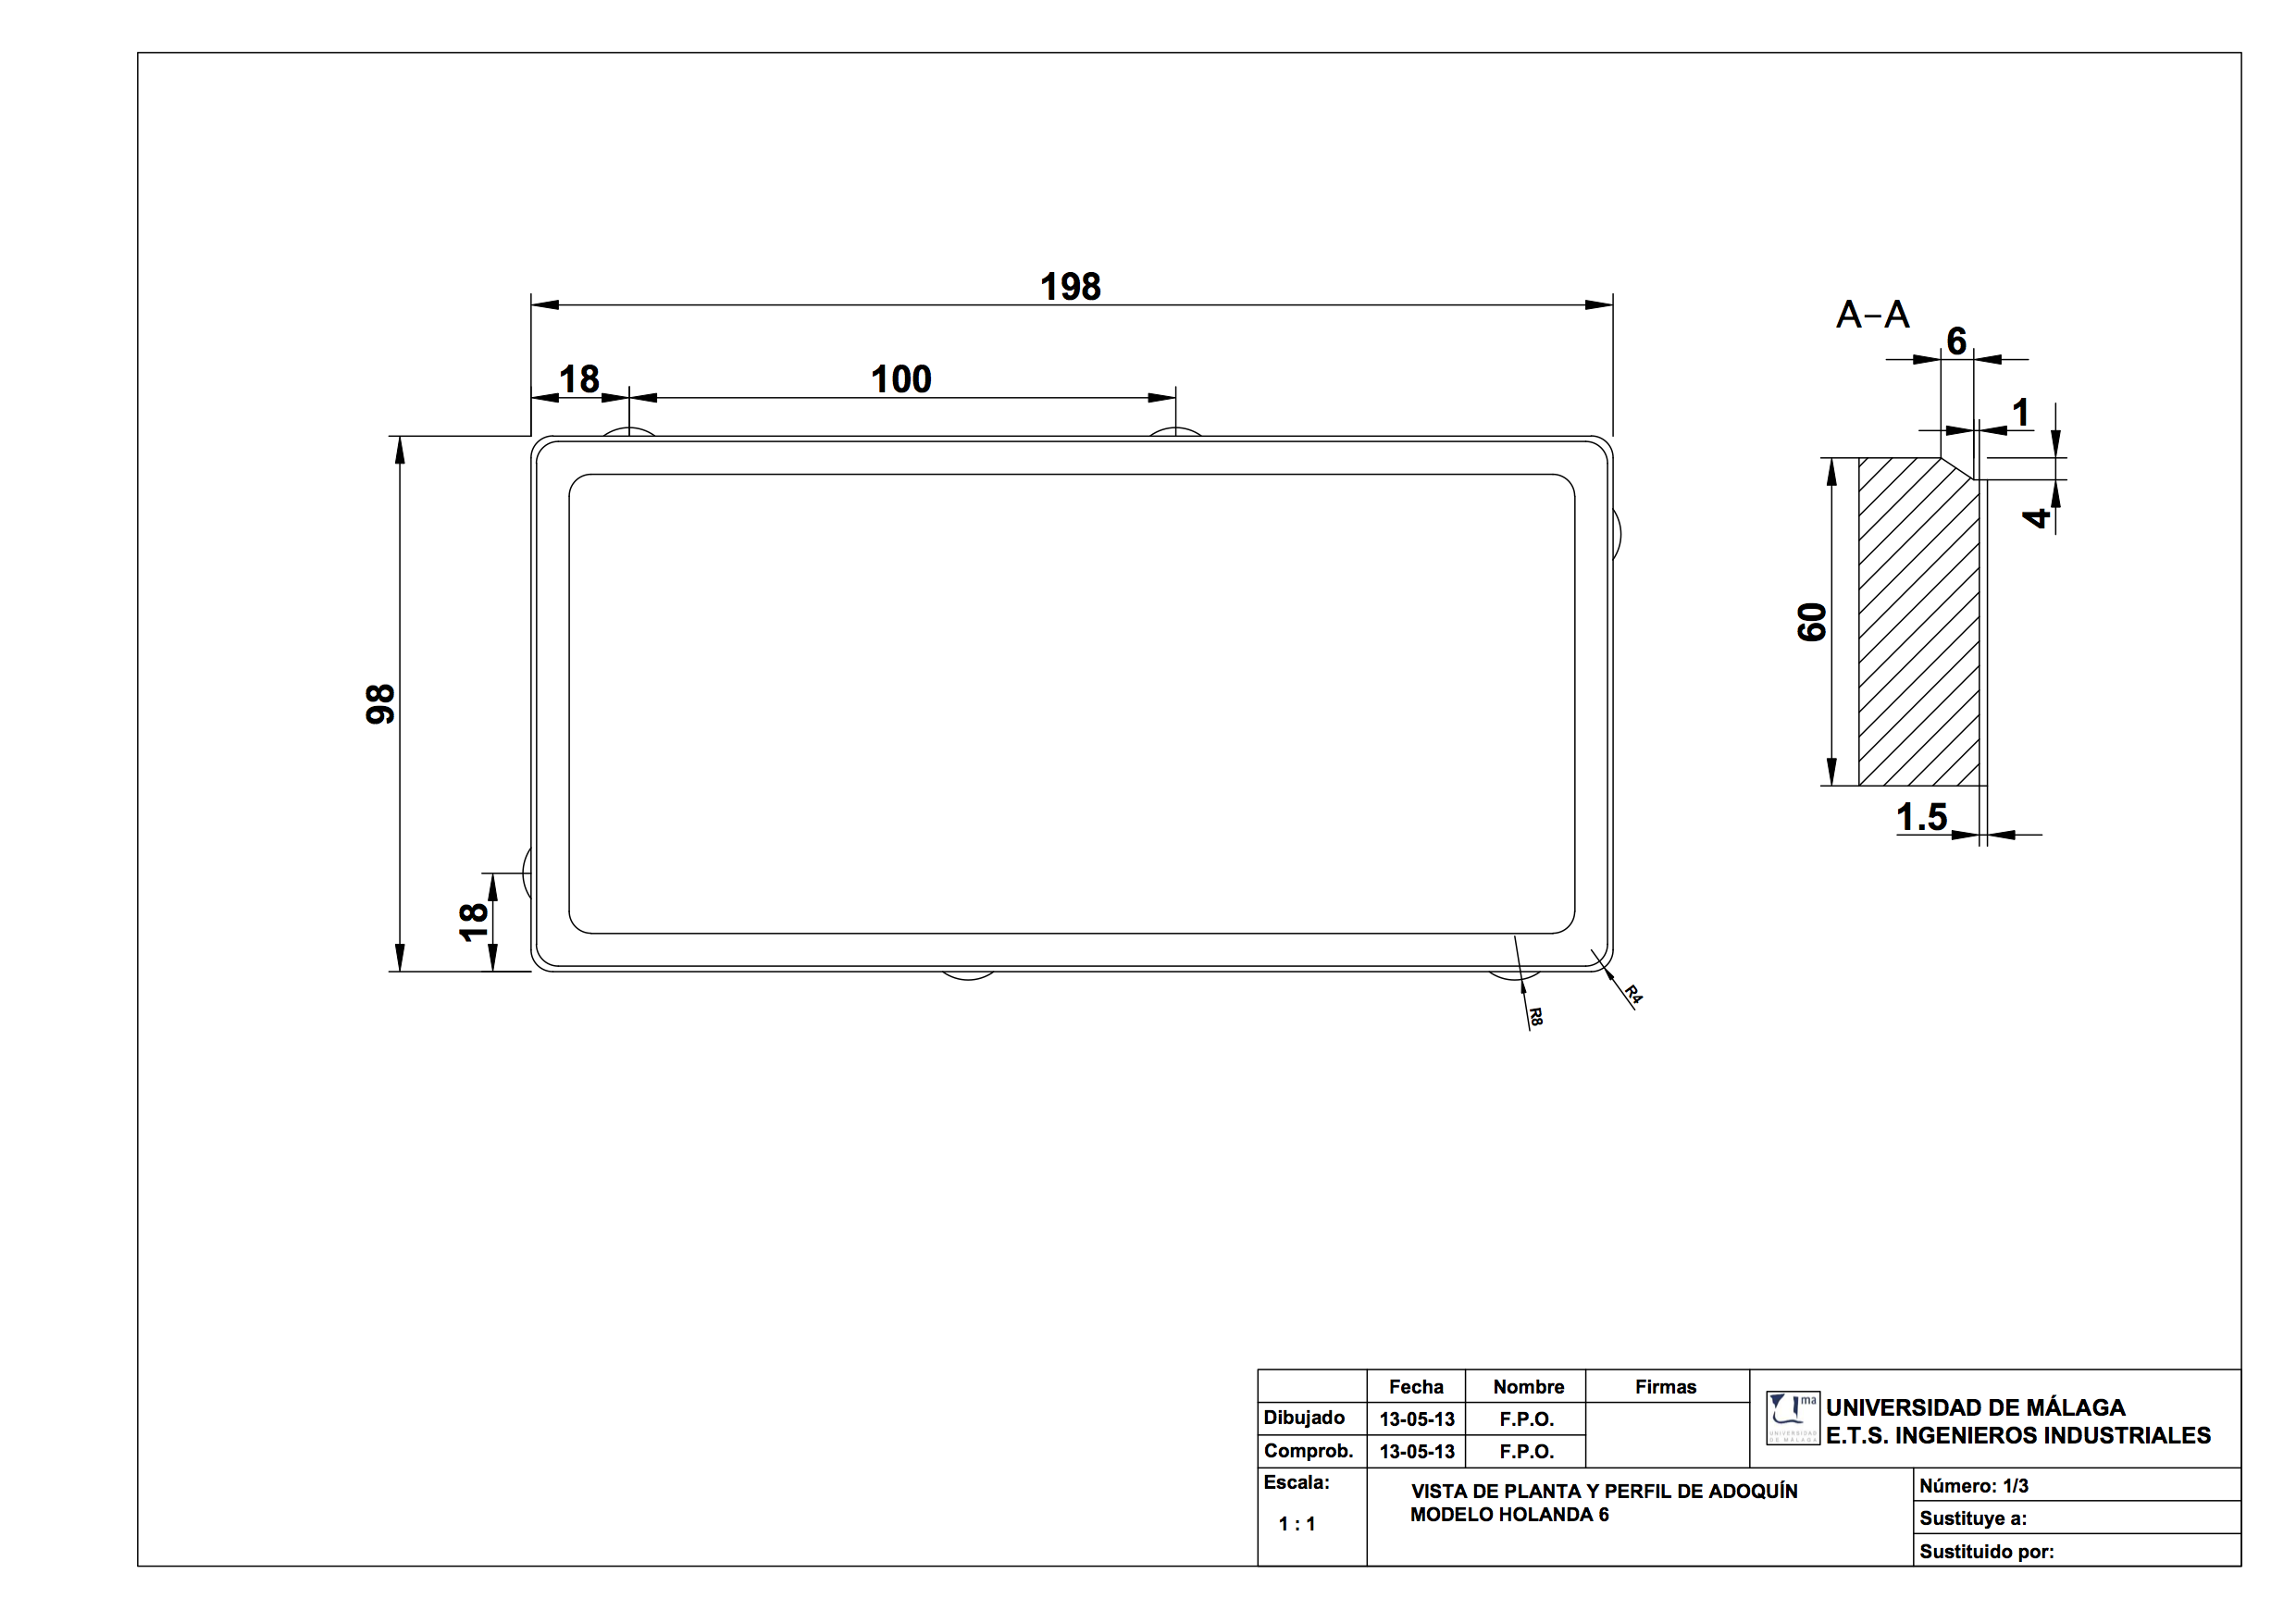
\includegraphics[angle=90,width=13.5cm]{plano_adoquin.png}
\end{figure}

\newpage
\setcounter{chapter}{2}
\addcontentsline{toc}{chapter}{\protect\numberline{\thechapter}Plano molde adoquín Holanda 6}
\begin{figure}[!htb]
\centering
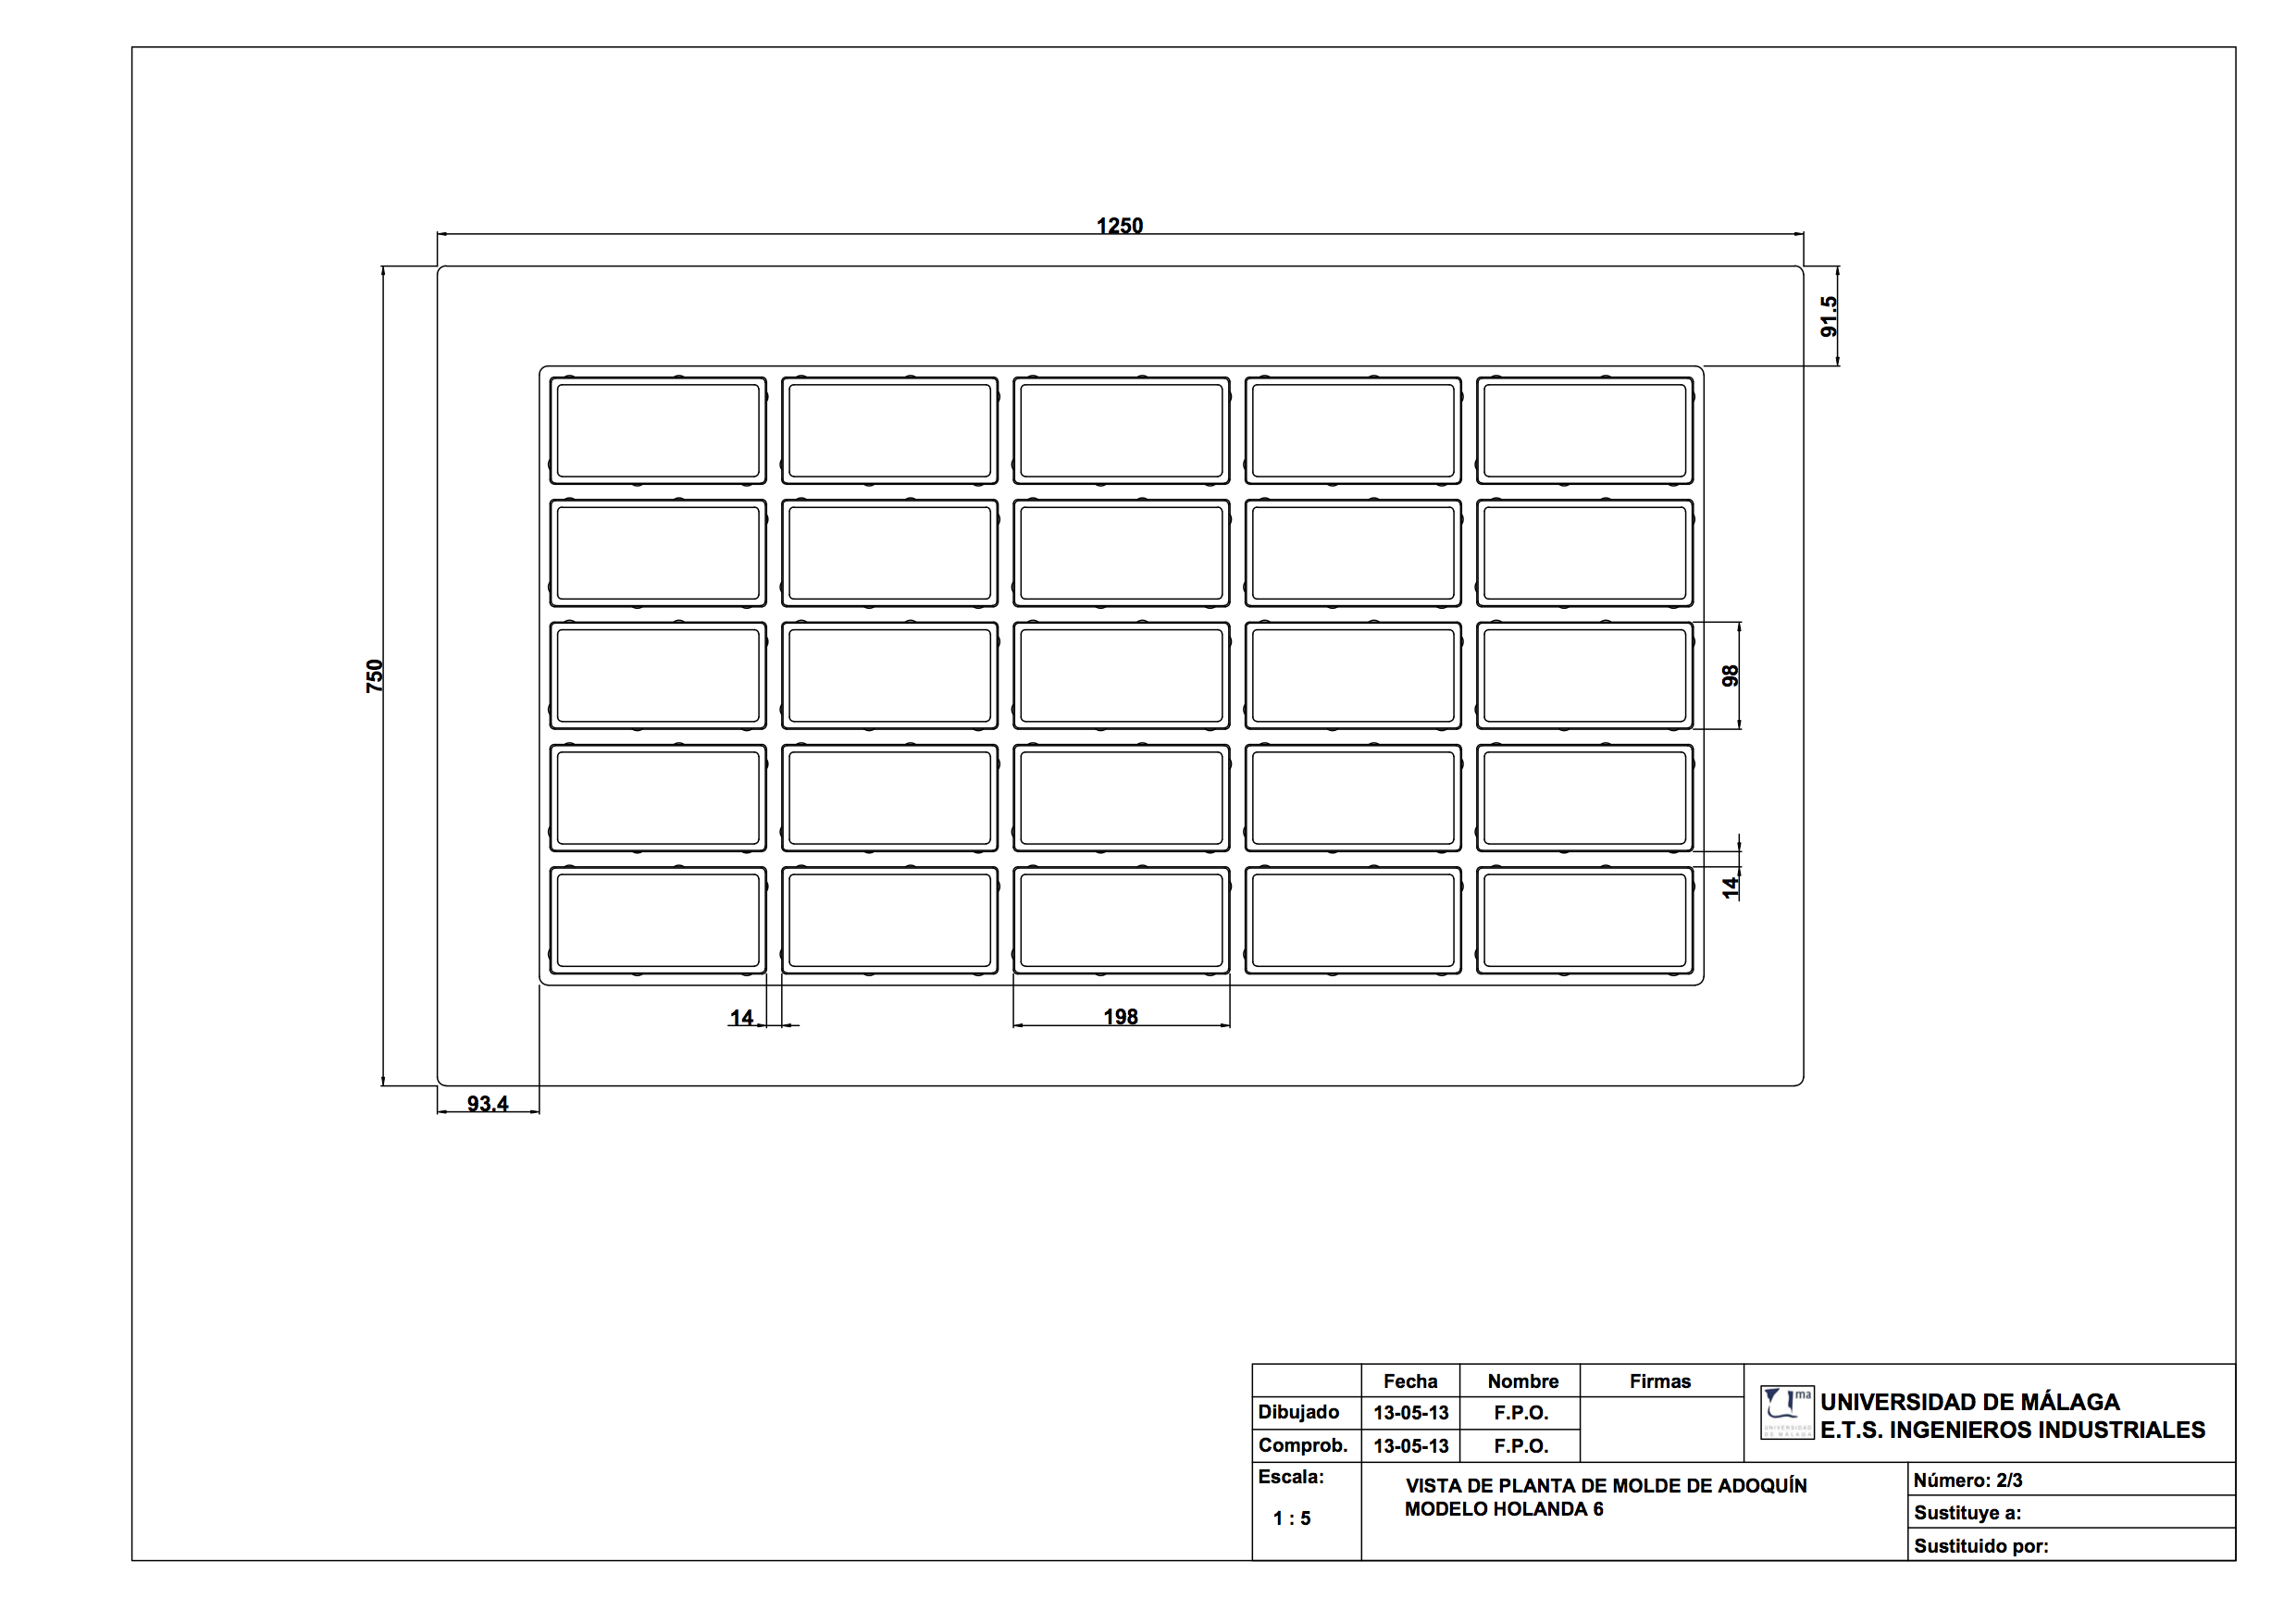
\includegraphics[angle=90,width=13.5cm]{plano_molde.png}
\end{figure}

\newpage
\setcounter{chapter}{3}
\addcontentsline{toc}{chapter}{\protect\numberline{\thechapter}Plano de instalaciones}
\begin{figure}[!htb]
\centering
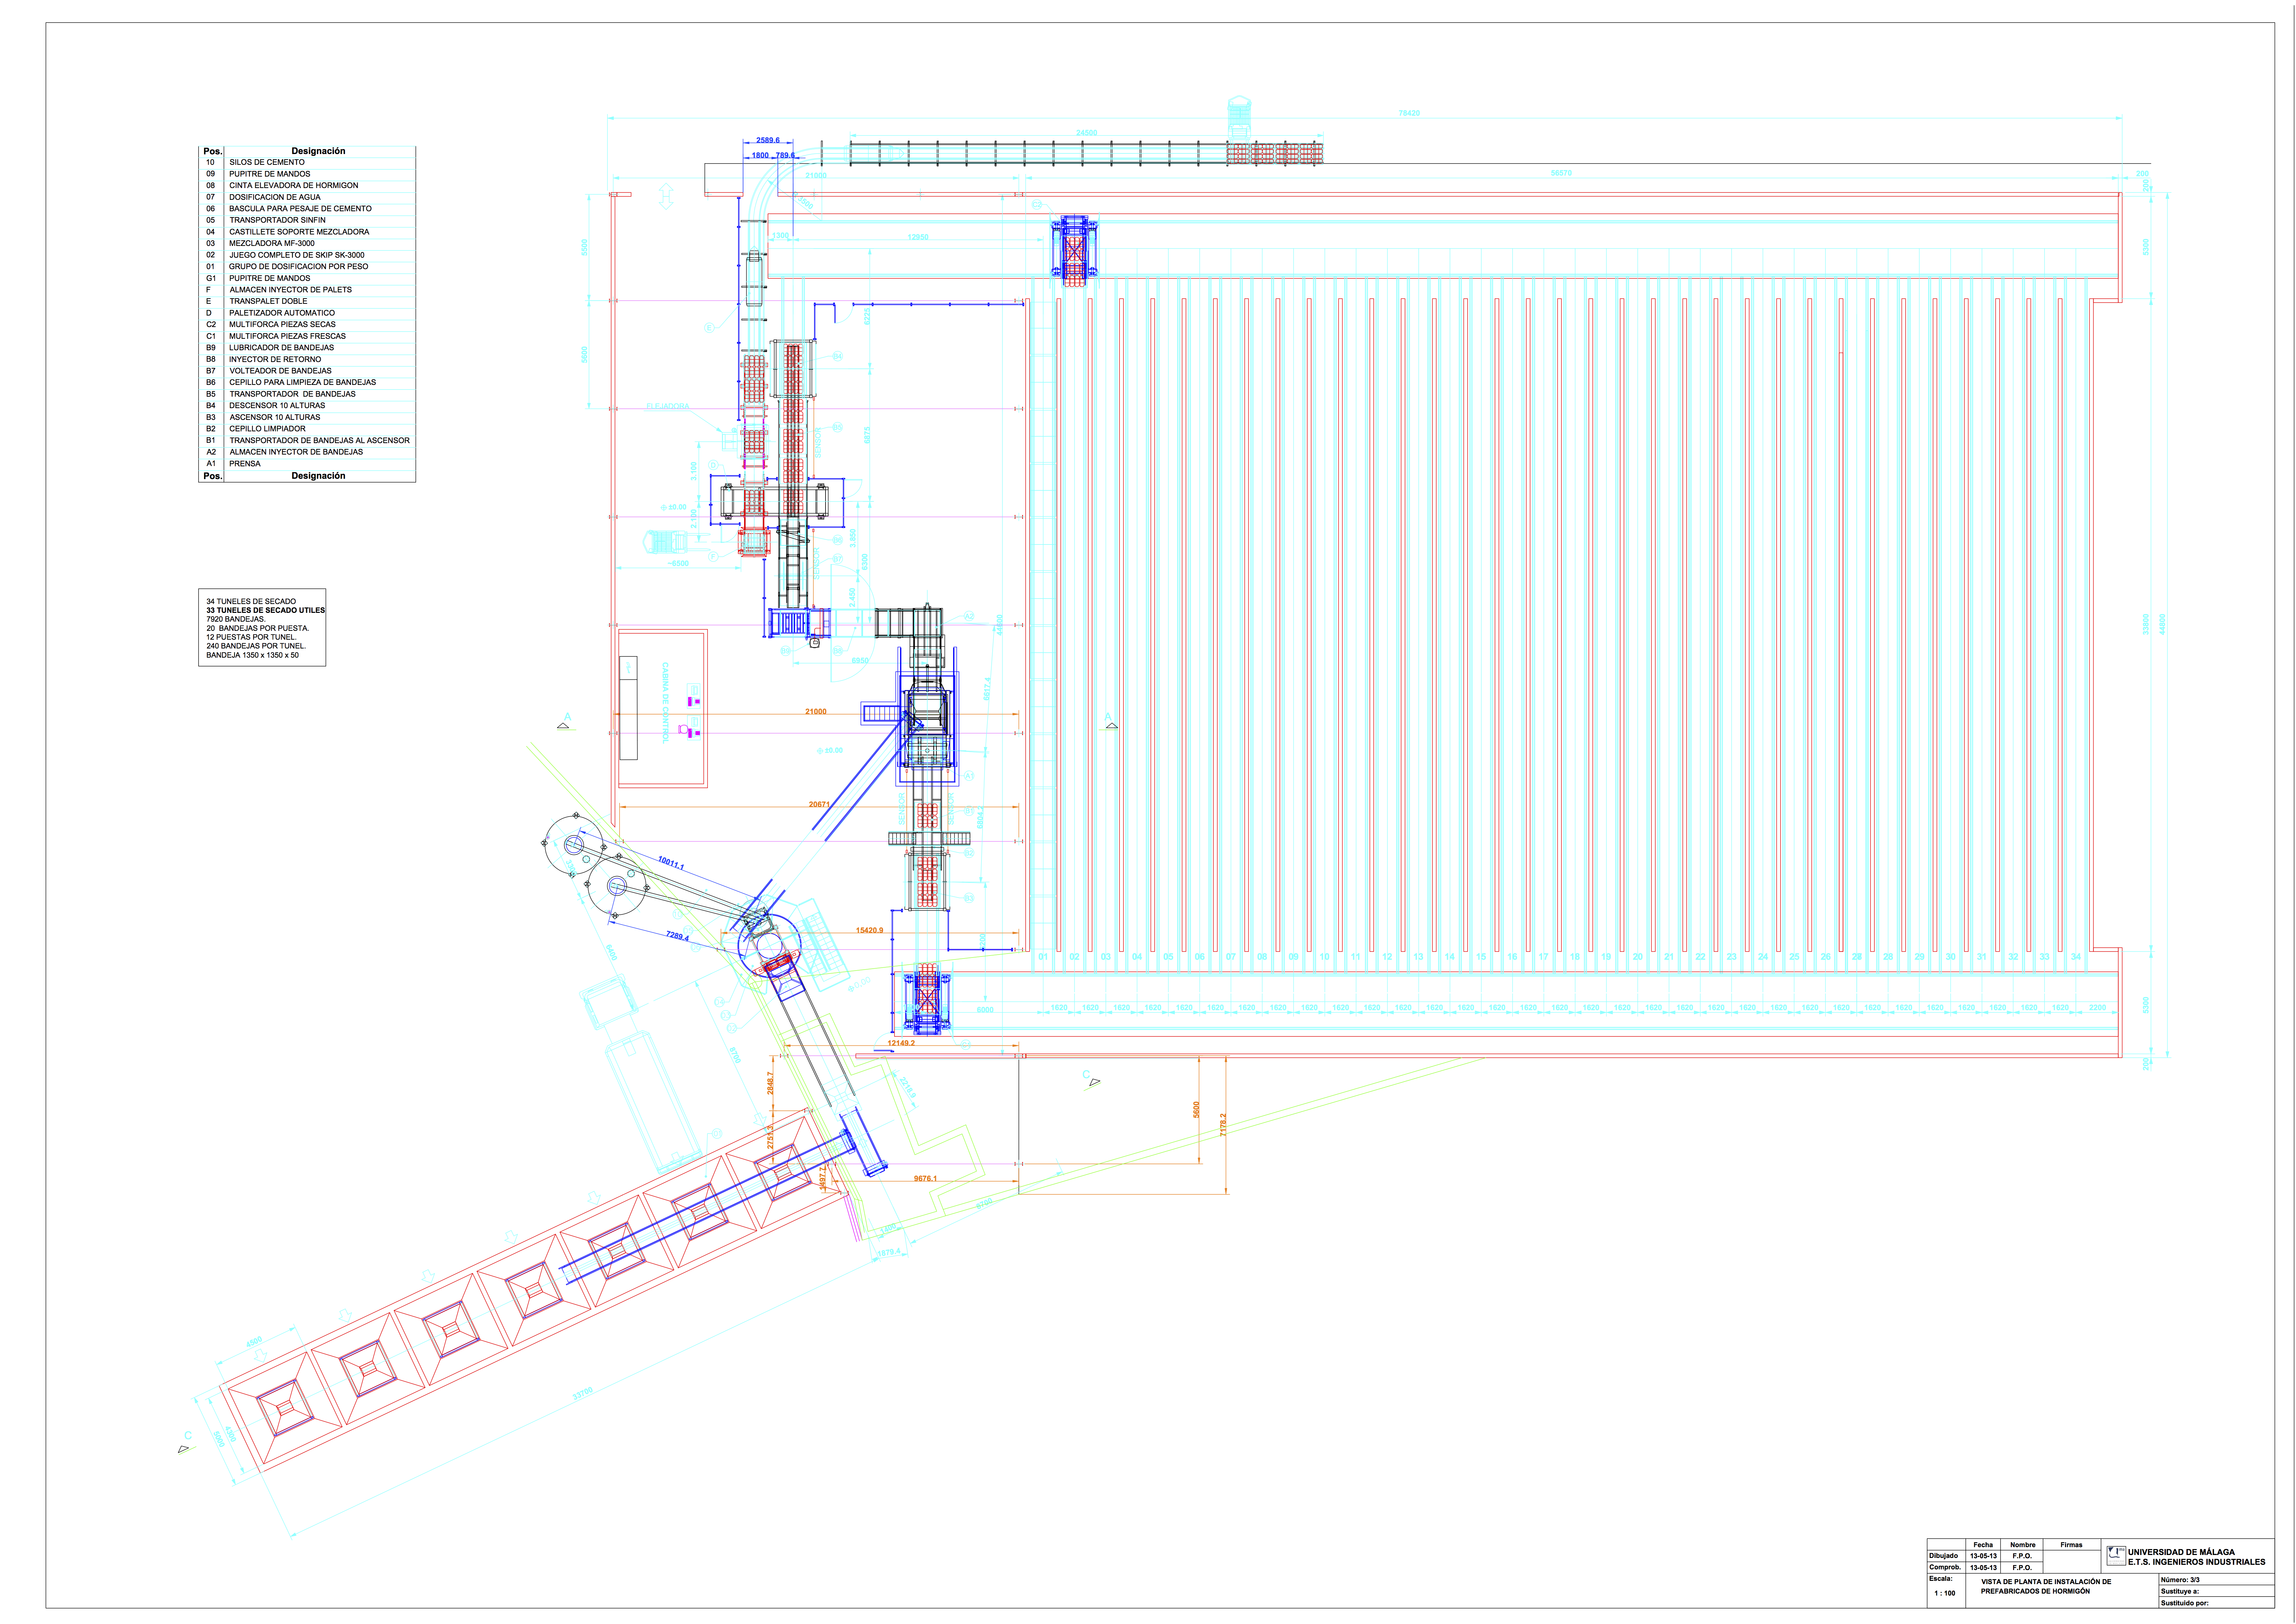
\includegraphics[angle=90,width=13.5cm]{plano_nave.png}
\end{figure}

\cleardoublepage

\part{Pliego de condiciones}
\parttoc
%!TEX root = informe.tex

\setcounter{chapter}{0}
\chapter{Condiciones técnicas}
% \addcontentsline{toc}{chapter}{Condiciones técnicas}

\section{Generalidades}

Los principios del Análisis de Ciclo de Vida son fundamentales y se deberán utilizar como orientación para tomar decisiones relacionadas tanto con la planificación como con la realización del análisis.

\section{Apreciación general del ciclo de vida}

El Análisis de Ciclo de Vida considerará el ciclo de vida completo del producto, desde la extracción y adquisición de la materia prima, pasando por la producción de energía y materia, y la fabricación, hasta el uso y el tratamiento al final de la vida útil y la disposición final. A través de esta visión general, se identificará y intentará evitar el desplazamiento de una carga ambiental potencial entre las etapas del ciclo de vida o los procesos individuales.

\section{Enfoque ambiental}
El Análisis de Ciclo de Vida tratará los aspectos e impactos ambientales del sistema del producto. Los aspectos e impactos económicos y sociales estarán fuera del alcance del Análisis de Ciclo de Vida. Se podrán combinar otras herramientas con el Análisis de Ciclo de Vida para análisis más profundos.

\section{Enfoque relativo y Unidad Funcional}
El Análisis de Ciclo de Vida será un enfoque relativo, que se estructurará alrededor de una Unidad Funcional. Esta Unidad Funcional definirá el estudio. Todos los análisis subsecuentes serán, por tanto, relativos a esa Unidad Funcional, ya que todas las entradas y salidas en el Inventario de Ciclo de Vida (ICV), y consecuentemente el perfil de la Evaluación del Impacto del Ciclo de Vida (EICV), se relacionarán con la Unidad Funcional.

\section{Enfoque iterativo}
El Análisis de Ciclo de Vida será una técnica iterativa. Las fases individuales del Análisis de Ciclo de Vida utilizarán resultados de las otras fases. El enfoque iterativo en y entre las fases contribuirá a la integridad y coherencia del estudio y de los resultados presentados.

\section{Transparencia}
Debido a la complejidad inherente al Análisis de Ciclo de Vida, la transparencia será un principio guía importante en la realización del Análisis de Ciclo de Vida, a fin de asegurar una adecuada interpretación de los resultados.

\section{Integridad}
El Análisis de Ciclo de Vida considerará todos los atributos o aspectos del entorno natural, de la salud humana y de los recursos. La consideración en un único estudio y con una perspectiva transversal de todos los atributos y aspectos, se podrán identificar y evaluar las compensaciones potenciales.

\section{Prioridad del enfoque científico}
Las decisiones en el Análisis de Ciclo de Vida se basarán preferentemente en las ciencias naturales. Si esto no es posible, se podrán utilizar otros enfoques, como las ciencias económicas y sociales, o se puede hacer referencia a convencio- nes internacionales. Si no existiera una base científica ni una justificación basada en otros enfoques o en convenciones internacionales, las decisiones se podrán basar en juicios de valor.

\section{Alcance}
Cuando se defina el alcance del Análisis de Ciclo de Vida, se considerará el contexto de la toma de decisión; es decir, los sistemas del producto estudiados deberán tratar adecuadamente los productos y procesos afectados por la aplicación prevista.

Los ejemplos de aplicación se referirán a decisiones que pretendan conseguir mejoras ambientales, lo que también constituye el enfoque global de la serie ISO 14000. Por lo tanto, los productos y procesos estudiados en un Análisis de Ciclo de Vida son aquellos afectados por la decisión que el Análisis de Ciclo de Vida pretende apoyar.

\chapter{Condiciones administrativas y legales}
% \addcontentsline{toc}{chapter}{Condiciones administrativas y legales}

\section{Autoría}
El autor de este proyecto cede al 50\% los derechos derivados de este proyecto al Departamento de Expresión Gráfica, Diseño y Proyectos de la Escuela Técnica Superior de Ingeniería Industrial de la Universidad de Málaga.

\section{Realización y supervisión}
El presente proyecto será realizado por el autor del mismo, bajo dirección y supervisión del tutor. Si esto no fuera posible, dicha realización y asesoría debería ser llevada a cabo por personal del Departamento de Expresión Gráfica, Diseño y Proyectos de la Escuela Técnica Superior de Ingeniería Industrial de la Universidad de Málaga.

\section{Cambios y desarrollos posteriores}
El autor del presente proyecto deberá ser puntualmente informado de los posibles cambios o modificaciones que pudiesen realizarse en el mismo.

En el caso de cambios o desarrollos posteriores de este proyecto se informará al autor para colaborar en el estudio o investigación que se este realizando.

\section{Consultas}
Se autoriza la consulta de este proyecto a toda persona autorizada por parte del Departamento de Expresión Gráfica, Diseño y Proyectos y a cualquier persona matriculada en la Universidad de Málaga que podrá solicitar el Proyecto en la Biblioteca de la Escuela Técnica Superior de Ingeniería Industrial de la Universidad de Málaga.

\vspace{1cm}
\today \hfill Fdo. Francisco José Pinto Oliver

\cleardoublepage

\part{Presupuesto}
\parttoc
%!TEX root = informe.tex
\chapter*{Coste de materiales}
\addcontentsline{toc}{chapter}{Coste de materiales}
Se contabilizarán todos los costes —en euros— relacionados con recursos materiales tales como material de oficina, software y hardware informático.

Respecto al material de oficina, abarca desde el soporte en papel para la impresión de documentación, fotocopias, encuadernación de este proyecto, soporte óptico que acompaña a este proyecto, planos hasta los cartuchos de tinta para su impresión.

El apartado de equipo informático engloba una licencia de sistema operativo, un procesador de textos para la redacción del presente proyecto, software para la creación de diagramas de flujo y tratamiento de imágenes.

En cuanto al software informático, se ha incluido una licencia para un único usuario tipo analista válida indefinidamente. Esto incluye el precio de la base de datos \textit{ecoinvent} versión 2 y la actualización a la versión 3. También incluye un año gratuito de soporte online y actualizaciones.

\begin{table}[!htb]
\centering
\begin{tabular}{lcrr}
\toprule
\multicolumn{4}{c}{Coste de materiales}\\
\midrule
Concepto & Cantidad & Importe (\euro) & Total (\euro)\\
\midrule
\multicolumn{2}{c}{Licencia SimaPro}\\
\cmidrule(r){1-2}
SimaPro single user, indefinite, Analyst & 1 & 8800.00 & 8800.00\\
ecoinvent Database & 1 & 0.00 & 0.00\\
Soporte y actualizaciones (1 año) & 1 & 0.00 & 0.00\\
\multicolumn{2}{c}{Equipo informático}\\
\cmidrule(r){1-2}
Ordenador portátil & 1 & 1329.00 & 1329.00\\
Procesador de texto & 1 & 0.00 & 0.00\\
Hoja de cálculo & 1 & 8.99 & 8.99\\
Software diagramas & 1 & 0.00 & 0.00\\
\multicolumn{2}{c}{Material de oficina}\\
\cmidrule(r){1-2}
DIN-A4 (500 uds.) & 1 & 5.50 & 5.50\\
Cartucho tinta negra & 1 & 18.00 & 18.00\\
Cartucho tinta color & 1 & 23.00 & 23.00\\
Encuadernación de tornillo & 1 & 12.00 & 12.00\\
Disco óptico DVD-R & 3 & 0.50 & 1.50\\
\bottomrule
Subtotal materiales & & & 10197.99\\
\bottomrule
\end{tabular}
% \caption{Presupuesto de materiales.}
\label{presupuestomateriales}
\end{table}

\chapter*{Coste de desarrollo}
\addcontentsline{toc}{chapter}{Coste de desarrollo}
El coste de desarrollo abarca los recursos humanos —en horas— necesarios para la realización del presente proyecto, documentación, recopilación de datos, redacción y correcciones del proyecto.

\begin{table}[!htb]
\centering
\begin{tabular}{lcrr}
\toprule
\multicolumn{4}{c}{Coste de desarrollo}\\
\midrule
Concepto & Cantidad (h) & Importe (\euro) & Total (\euro)\\
\midrule
\multicolumn{2}{c}{Documentación}\\
\cmidrule(r){1-2}
Documentación & 130 & 19.00 & 8800.00\\
Entrevista con fabricante & 17 & 19.00 & 0.00\\
Consultas varias & 11 & 19.00 & 0.00\\
\multicolumn{2}{c}{Redacción del proyecto}\\
\cmidrule(r){1-2}
Redacción & 170 & 19.00 & 5.50\\
Introducción del modelado & 60 & 19.00 & 18.00\\
Corrección de errores & 35 & 19.00 & 23.00\\
\bottomrule
Subtotal desarrollo & & & 8037.00\\
\bottomrule
\end{tabular}
% \caption{Presupuesto de desarrollo.}
\label{presupuestodesarrollo}
\end{table}

\chapter*{Presupuesto general}
\addcontentsline{toc}{chapter}{Presupuesto general}

\begin{table}[!htb]
\centering
\begin{tabular}{lcrr}
\toprule
\multicolumn{4}{c}{Coste total del proyecto}\\
\midrule
Concepto & Cantidad & Importe (\euro) & Total (\euro)\\
\midrule
Subtotal materiales & & & 10197.99\\
Subtotal desarrollo & & & 8037.00\\
\bottomrule
Total & & & 18234.99\\
\bottomrule
\end{tabular}
% \caption{Coste total del proyecto.}
\label{presupuestototal}
\end{table}

\begin{table}[!htb]
\centering
\begin{tabular}{lcrr}
\toprule
\multicolumn{4}{c}{Presupuesto general}\\
\midrule
Concepto & Cantidad (\%) & Importe (\euro) & Total (\euro)\\
\midrule
Coste total del proyecto & & & 18234.99\\
Gastos generales & 13 & & 2370.55\\
Beneficio industrial & 6 & & 1094.10\\
I.V.A. & 21 & & 3829.35\\
\bottomrule
Total & & & 25528.99\\
\bottomrule
\end{tabular}
% \caption{Presupuesto general.}
\label{presupuestogeneral}
\end{table}

\end{document}

